\documentclass{thesisreport}

\setcounter{tocdepth}{3}
\setcounter{secnumdepth}{3}

\usepackage{caption}
\usepackage{subcaption}
\usepackage{comment}
\usepackage{amsmath}
\usepackage{bm}
\usepackage{multicol}
\usepackage{xcolor}
\usepackage{tabularx}
\usepackage{optidef}
\usepackage{mathtools}

\setlength{\columnseprule}{1pt}
\def\columnseprulecolor{\color{black}}
\DeclareUnicodeCharacter{2212}{-}

\setlength\parindent{0pt}

\begin{document}

 \thispagestyle{empty}

\def\lskip{\vspace{0.5cm}}


\begin{tabular}{p{7cm}p{8cm}}
ÉCOLE CENTRALE DE NANTES
&
% EMARO students only
% \raggedleft FIRST YEAR INSTITUTION	
\end{tabular}

\vspace{2cm}

% CORO-IMARO students
\begin{center} \large\sc MASTER CORO-IMARO\\ \normalsize{``CONTROL and ROBOTICS''} \end{center}

% EMARO students
%\begin{center} \large\sc MASTER ERASMUS MUNDUS \\ \normalsize{EMARO+ ``European Master in Advanced Robotics''} \end{center}


\begin{center}
	2016 / 2017\\
	\lskip
	Master Thesis Report % or bibliography report
	\lskip
	
	Presented by \lskip 
	
	Student Name \lskip
	
	On Date \lskip\lskip
	
	{\Large \textbf{The title of the master thesis}}
	
	\vfill

Jury \lskip
		
	\end{center}
	


\begin{tabular}{p{3cm}p{7cm}p{5cm} }
 % President: & Name & Position (Institution) \\ & & \\     % for final defense only (not bibliography)
 Evaluators: & Name & Position (Institution) \\
	      & Name & Position (Institution) \\ 
	      & Name & Position (Institution) \\ & & \\  & & \\ 
  Supervisor(s):  & Name & Position (Institution) \\
		  & Name & Position (Institution) \\
% EMARO students only
%(EMARO)  & Co-supervisor from M1 & Position, M1 institution 
\end{tabular}

\lskip

\begin{flushleft}
 Laboratory: Laboratoire des Sciences du Numérique de Nantes LS2N
\end{flushleft}

\newpage
\thispagestyle{empty}
\null
\newpage
\addtocounter{page}{-1}
\pagestyle{fancy}
  
 
  \section*{Abstract}
Within the rapidly growing aerial robotics market, one of the most substantial challenges in the quadrotor community is performing aggressive maneuvers, especially multi-flip maneuvers.  A proper physical definition of the issue is not addressed by the current approaches in the field and several key aspects of this maneuver are still overlooked.
It can be shown, in particular, that making a flip with a quadrotor means crossing the parallel singularity of the dynamic model. The aim of the master thesis is to explore the possibility of defining aggressive trajectories for quadrotors on the basis of their dynamic model degeneracy analysis and to adapt various strategies to control the robot in a closed loop. In addition, the possibility to perform the aggressive maneuver in constrained environments will also be investigated.
Therefore, the analysis will be extended from the previous studies to create general feasible trajectories that will allow quadrotors to perform aggressive multi-flip maneuvers while passing through a constrained environment and while guaranteeing a satisfactory degree of robustness to the uncertainties of the dynamic model.\\

\textbf{Keywords: quadrotors, parallel robots, aggressive maneuvers, multi-flips, constrained environmen. } 
 
 \newpage
 
 \section*{Acknowledgements}


I would like to express my special thanks and gratitude to my supervisors Dr. Sébastien Briot and Dr. Isabelle Fantoni who gave me the  opportunity to work on this wonderful project which encapsulates control theory, dynamics and quadrotors. This project has allowed me to perform research on all of these topics and I am now more knowledgeable thanks to my supervisors. Moreover, I would like to thank them for believing in my capabilities and giving me the confidence and the support when I needed it. \\\\
Secondly, I would also like to thank Dr. Ina Taralova for providing me with the valuable knowledge to create a proper bibliography. \\\\
I would like to thank my patient and understanding girlfriend Glysa, who has been with me for more than 5 years. Thank you for all the love, support and comfort that you have given me in these stressful 2 years. I hope that this Master degree will allow us to have a better future together. \\\\
I would like to thank my family as well: my parents Naji and Yolla, my sister Rebecca, my uncle and his wife Fadi and Lara and my aunt Bernadette. They have provided me with the emotional and economical support from the very beginning and they gave me the opportunity to travel and study for this Master degree. They have always been proud and encouraging. \\I would not be here if it wasn't for them.

 
 \newpage
 
 
 \section*{Notations}
 \begin{tabular}{cp{0.8\textwidth}}
 $M_i$ & motor $i$\\
 $J_r$ & rotor inertia\\
  $\overrightarrow{f_i}$ & lift due to $M_i$\\
  $b$ & thrust factor \\
  $d$ & drag coefficient \\
  $\omega$ & angular velocity according to $(G,  \overrightarrow{a_G})$ axis of the vehicle \\
$\omega_i$ & rotation velocity of motor $Mi$\\
$\omega_r$ & overall residual propeller angular speed\\
$\psi$ & yaw angle\\
$\theta$ & pitch angle\\  
  $\phi$ & roll angle\\
  $l$ & horizontal distance: from the center of the propeller to the CoG \\
  $\tau$ & resulting torque of the quadrotor\\
  $\tau_a$ & rotational torque of the quadrotor\\
  $\tau_G$ & rotational torque due to the gyroscopic effects of the rotors\\
  ${}^{O}A_M$ & transformation matrix from the mobile frame $M$ to the fixed frame $O$\\
  ${}^{M}A_O$ & transformation matrix from the mobile frame $O$ to the fixed frame $M$\\
  $CT$ & continuous time \\
  $DT$ & discrete time \\
  $R_O$ & Working frame related to the environment\\
  $R_M$ & general mobile frame\\
  $R_U$ & UAV frame\\
  $X$ & A vector expressed in its proper frame\\
  ${}^{R}[X]$ & X expressed in the frame R\\
  $\xi = \begin{bmatrix}
  x && y && z 
  \end{bmatrix}^{\intercal}$ & Position of the center of mass vector and expressed in the fixed frame\\
  $\eta = \begin{bmatrix}
  p && q && r
\end{bmatrix}^{\intercal}$ & angular velocity vector of the UAV expressed in the robot frame.\\
$t_k$ & time at knot point $k$\\
$h_k=t_{k+1} - t_k$ & duration of spline segment $k$\\
$\bm{x}_k=\bm{x}(t_k)$ & state at knot point $k$\\
$\bm{u}_k=\bm{u}(t_k)$ & control at knot point $k$\\


\end{tabular}\\
 
 
 
 \newpage
 
  \section*{Abbreviations}
 \begin{tabular}{cp{0.8\textwidth}}
  \textbf{UAV} & unmanned aerial vehicle \\
  %\textbf{IGE} & in ground effect \\
  %\textbf{OGE} & out of ground effect \\
  \textbf{CoG} & center of gravity \\
  \textbf{i.s.L.} & in sense of Lyapunov \\
  \textbf{lpd} & locally positive definite \\
  \textbf{lpsd} & locally positive semi-definite \\
  \textbf{lnd} & locally positive negative definite \\
  \textbf{MPC} & model predictive control \\
\end{tabular}\\
 \newpage
 
 \listoffigures
 
\listoftables
 
 \tableofcontents
 
 
 \chapter*{Introduction}
 \addcontentsline{toc}{chapter}{Introduction}	 % non-numbered chapters do not appear in table of contents by default
 	The aim of this section is to provide a general summary of the robotic platform that is used for this master thesis and to illustrate the main objective of the research work.
In specific, in the sections below, quadrotors and parallel robots are briefly presented.


 
 
 \section*{The quadrotor platform}

A quadrotor is a type of unmanned aerial vehicle (UAV) with four rotors and six degrees of freedom. Typically, drones have a small size and low inertia which allows them to be controlled by simple flight control systems. It is typically designed in a cross-configuration such that the electronics are held in the center of the platform and the rotors are placed at the borders.
An example of a real quadrotor, namely the DJI Phantom, is shown in fig. \ref{fig:drone}. The quadrotor is typically built in a way such that a pair of opposite rotors rotate clockwise, whereas the other pair of rotors rotates in counter-clockwise.
The attitude and the position of the drone are controlled by changing the spinning speed of the rotors. An example is shown in figure \ref{fig:propeller_directions}.



\begin{figure}[h]
     \centering
     \begin{subfigure}[b]{0.45\textwidth}
         \centering
         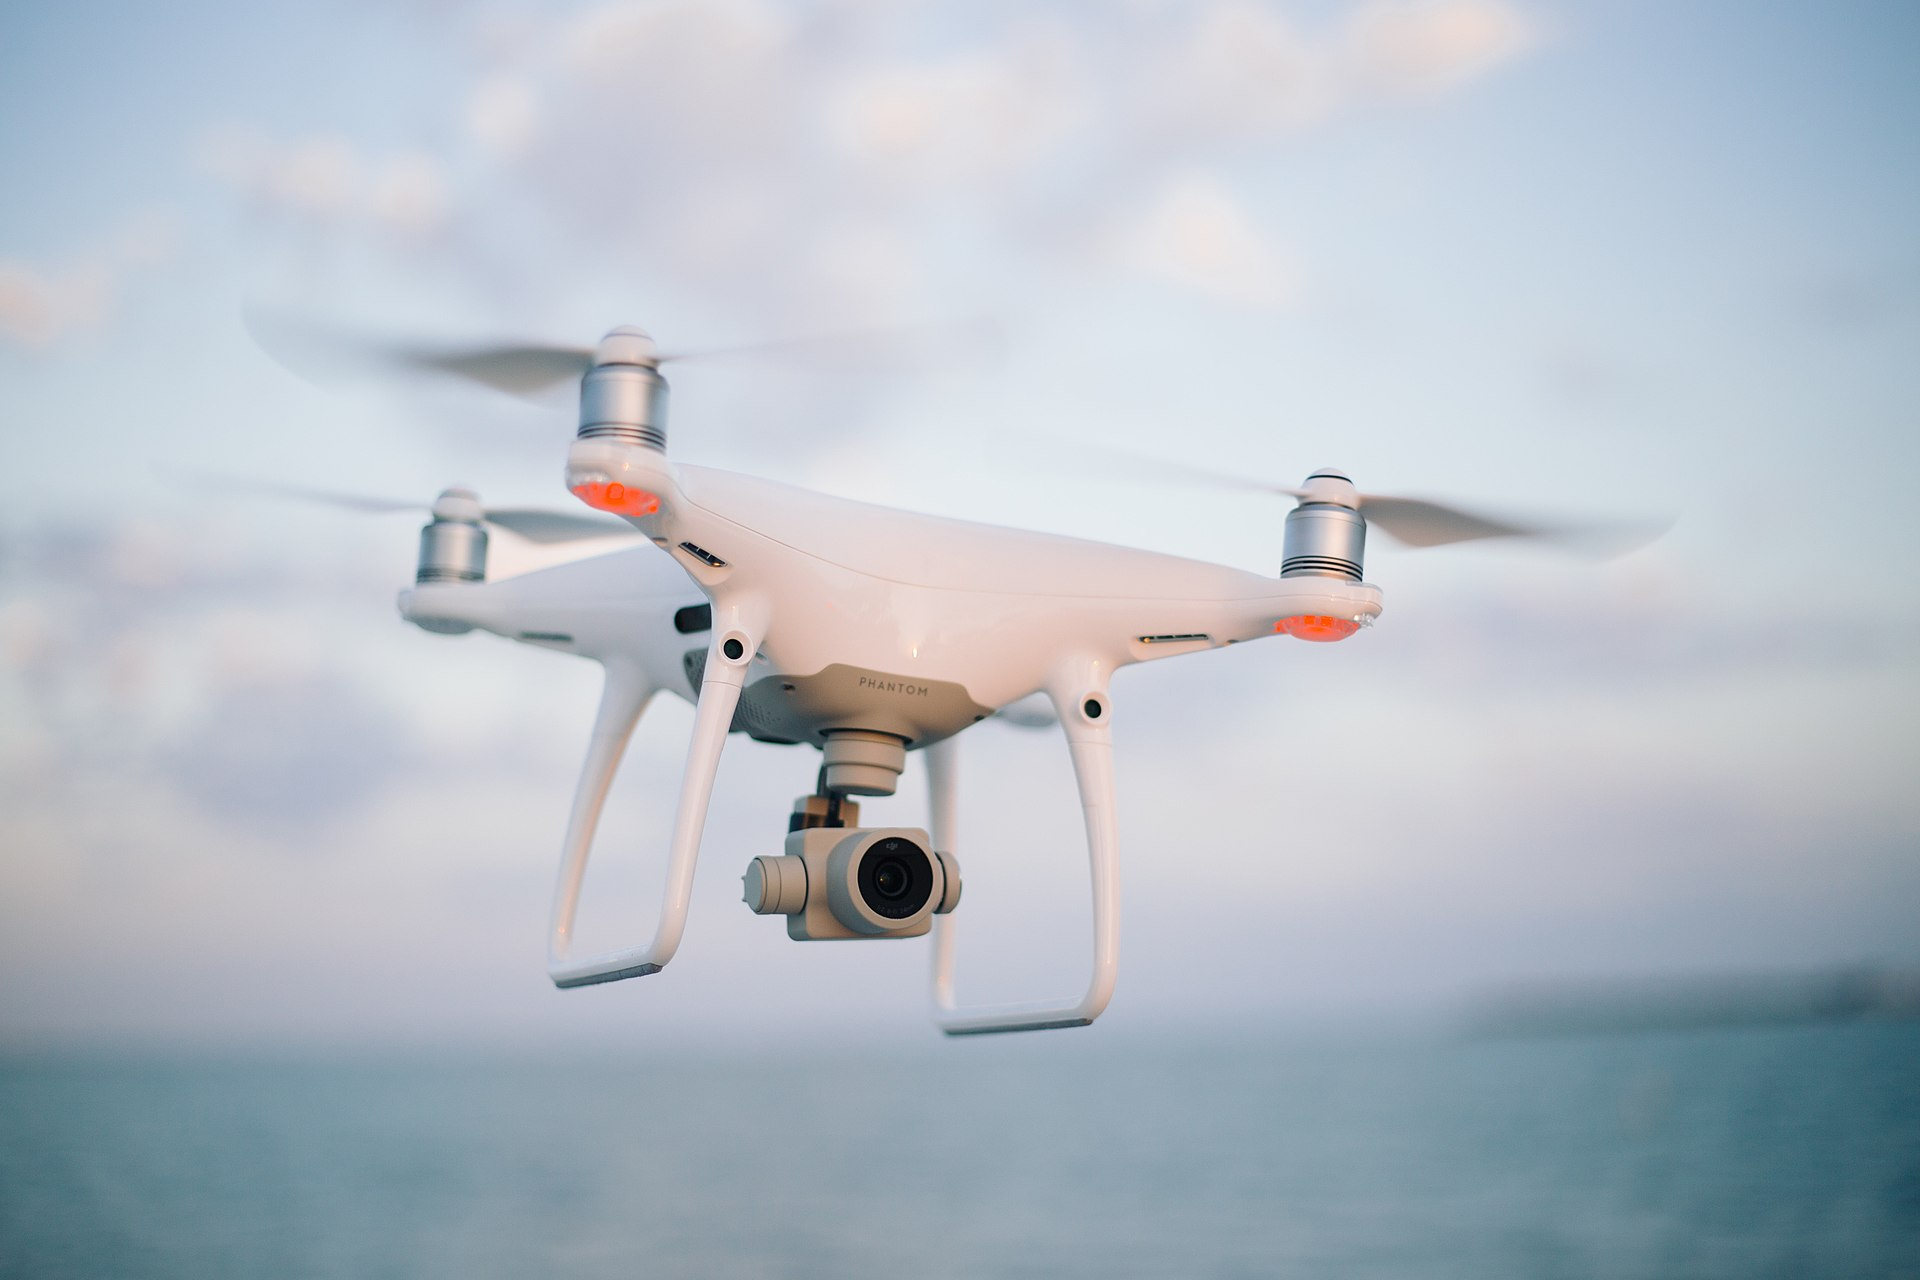
\includegraphics[width=\textwidth]{Images/Introduction/drone}
         \caption[Caption for LOF]{A DJI Phantom quadcopter (UAV)\protect\footnotemark}
         \label{fig:drone}
     \end{subfigure}
     \hfill
     \begin{subfigure}[b]{0.45\textwidth}
         \centering
         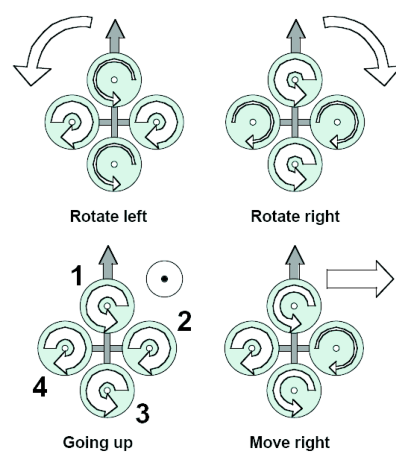
\includegraphics[width=0.6\textwidth]{Images/Introduction/propeller_direction.svg}
         \caption{Representation of the concept of a quadrotor. The width of the arrows is proportional to the angular speed of the propellers.\cite{Bouabdalla2007}}
         \label{fig:propeller_directions}
     \end{subfigure}
        \caption{A commercial quadrtotor platform with a representation of the quadrotor concept.}
        \label{fig:three graphs}
\end{figure}

\noindent The distinctive mechanical design of the quadrotor permits the actuation system to control all of the six degrees of freedom even though it is under-actuated. This is due to the fact that the rotational and translational dynamics are tightly coupled. Thus, all the translational and rotational motions can be carried off by properly controlling the magnitude and direction of the spinning speed of the rotors.   

\noindent \footnotetext[1]{\url{https://en.wikipedia.org/wiki/Quadcopter\#/media/File:Quadcopter_camera_drone_in_flight.jpg}, accessed on 01/08/2021.}


\pagebreak

Over the last few years, quadrotors have gained a large popularity in academia and in the industry. This is due to several reasons, such as: 

\begin{enumerate}

    \item Quadrotors are very simple to design and they can be easily assembled using relatively cheap components.  
    \item As quadrotors became more and more affordable and dependable, the number of real-world applications for quadrotors  has grown significantly. They are being used for aerial photography, agriculture, surveillance, inspection tasks, in addition to many other uses as well. 
    \item Quadrotors are quite agile and maneuverable during flight, especially when compared to other types of UAVs.
    
\end{enumerate}

However, one of the main challenges in the quadrotors community is the capability to design control and planning methods that will allow the quadrotors to carry out aggressive maneuvers.  The fast dynamics associated with typically small dimensions of such agile quadrotors, along with several aerodynamic effects that will become crucial during aggressive flight maneuvers, are just a few of the main problems that are faced during the system control design. Moreover, accurate tracking of the provided trajectory is a big issue in the case of aggressive maneuvers when the rotors are commanded high speeds and accelerations, which will cause rotors to become saturated and may also cause delays.


 \section*{Parallel manipulators}

A parallel manipulator is a mechanical system that consists of two connected platforms, the fixed platform and the moving platform. The latter is linked to the fixed platform thanks to at least two serial chains that are working in parallel. When compared to serial manipulators, parallel manipulators are more accurate and rigid. In addition, the ability to install the motors next to the fixed platform is a very important feature for parallel manipulators. Moreover, parallel manipulators can be used in a wide variety of applications that demand precision and high payload combined with high speed.\cite{Parallel_Manipulators}

\begin{figure}[h]
     \centering
     \begin{subfigure}[h]{0.45\textwidth}
         \centering
         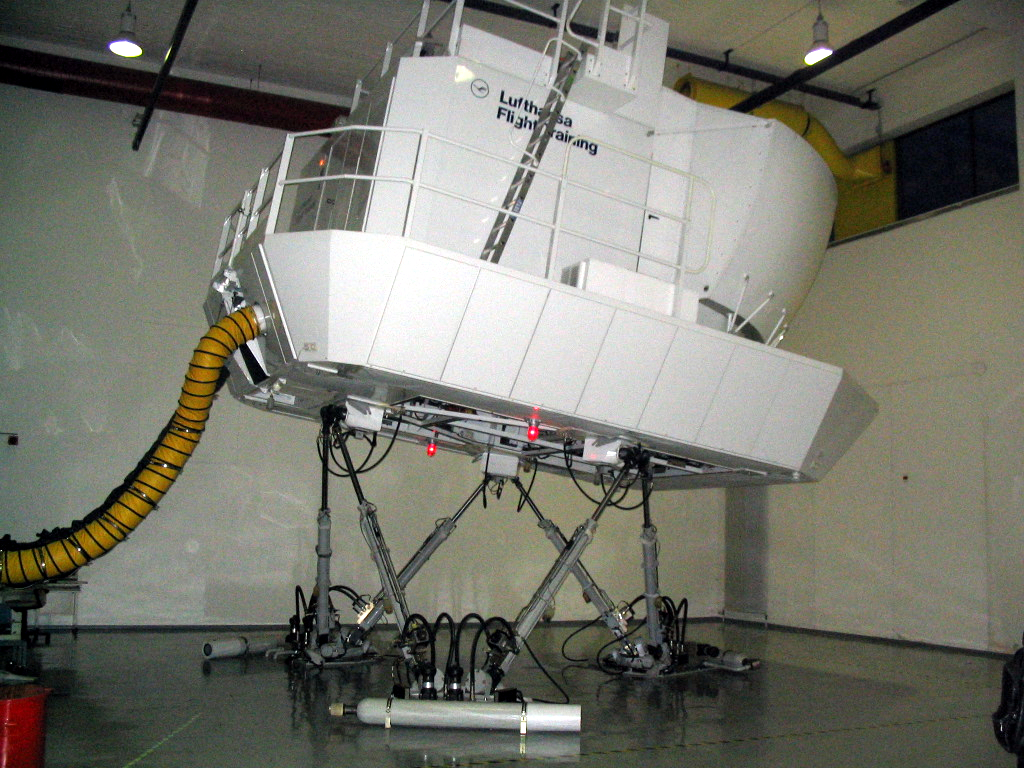
\includegraphics[width=0.7\textwidth]{Images/Introduction/GS}
    \caption[Caption for LOF]{Gough-Stewart used for a flight-simulator application.\protect\footnotemark}
         \label{GS}
     \end{subfigure}
     \hfill
     \begin{subfigure}[h]{0.45\textwidth}
         \centering
         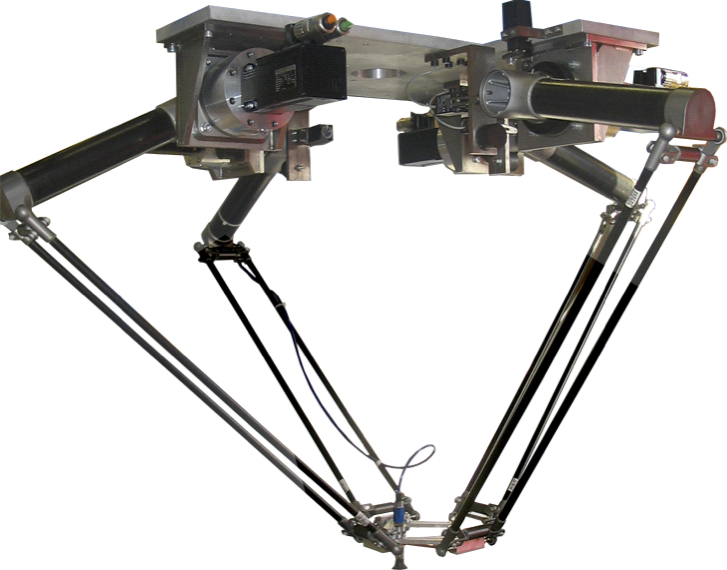
\includegraphics[width=0.7\textwidth]{Images/Introduction/PAR4}
         \caption[Caption for LOF]{The "PAR4" 4 degrees of freedom, high-speed, parallel robot prototype.\protect\footnotemark}
         \label{PAR4}
     \end{subfigure}
        \caption{Two examples of parallel robots.}
        \label{fig:three graphs}
\end{figure}




\footnotetext[1]{\url{https://en.wikipedia.org/wiki/Stewart_platform\#/media/File:Simulator-flight-compartment.jpeg}, accessed on 01/08/2021.}
\footnotetext[2]{\url{https://en.wikipedia.org/wiki/Parallel_manipulator\#/media/File:Prototype_robot_parall\%C3\%A8le_PAR4.jpg}, accessed on 01/08/2021.}


\pagebreak

However, parallel manipulators are subject to singularities which can lead to big problems in the robot workspace in case they were not handled correctly. Thus, the study of the singular configuartions of parallel manipulators is very important. Because, even just before reaching a singularity, the performance of the parallel manipulator will decrease dramatically. Moreover, the robot may loose the ability of moving in a certain direction, gain uncontrollable motions and the mechanism could even break. The main difference between serial and parallel manipulators is that singularity configurations may also appear inside the workspace of the robot (depending on the dimensions of the robot) and not just at the boundaries of the robot workspace, which can significantly decrease the area of the robot workspace.
As a result, many works have been developed by robotics researchers in order to allow parallel manipulators to safely cross these singularities by using trajectory planning and specific control methods.

\section*{The goal of this thesis}

This master thesis lies at the intersection of parallel robotics and aerial robotics. The two fields may seem very different from each other. However, quadrotors can be seen as a particular case of a parallel manipulator. 
In fact, a parallel manipulator is made up of a wrench system, applied by the robot limbs on the moving platform. And, this wrench system will define the motion of the moving platform. In the same manner, each propeller in a quadrotor can be considered as limb of a parallel robot and the moving platform to be controlled can be considered as the body of the drone. 
Specifically, the goal of this master thesis is to study a distinct class of aggressive maneuvers for quadrotors, namely multi-flip maneuvers. By doing multi-flip maneuvers, full rotations around one or more axes of the body of the quadrotor can be done. In addition, the quadrotor must also perform the multi-flip maneuvers in a constrained environment.

\begin{figure}[h]
     \centering
     \begin{subfigure}[h]{0.45\textwidth}
         \centering
         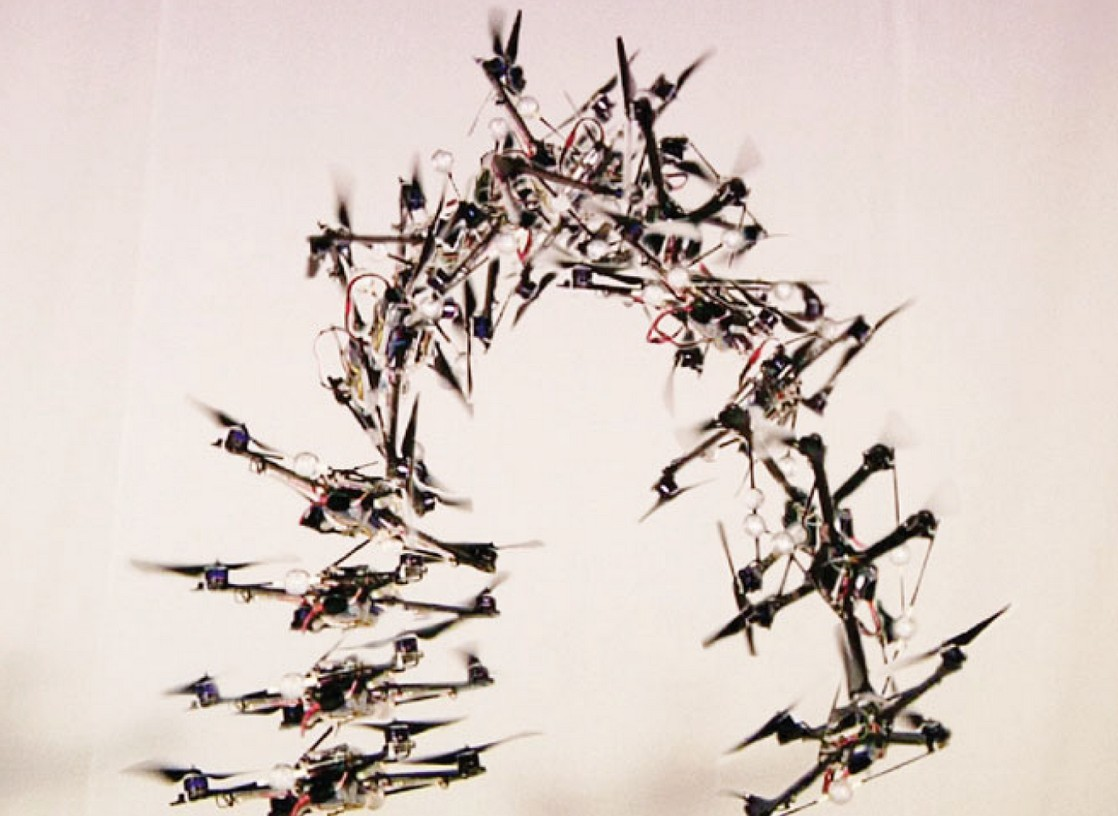
\includegraphics[width=0.9\textwidth]{Images/Introduction/flip}
    \caption{Quadrotor performing a triple flip.\cite{flip}}
         \label{triple_flip}
     \end{subfigure}
     \hfill
     \begin{subfigure}[h]{0.45\textwidth}
         \centering
         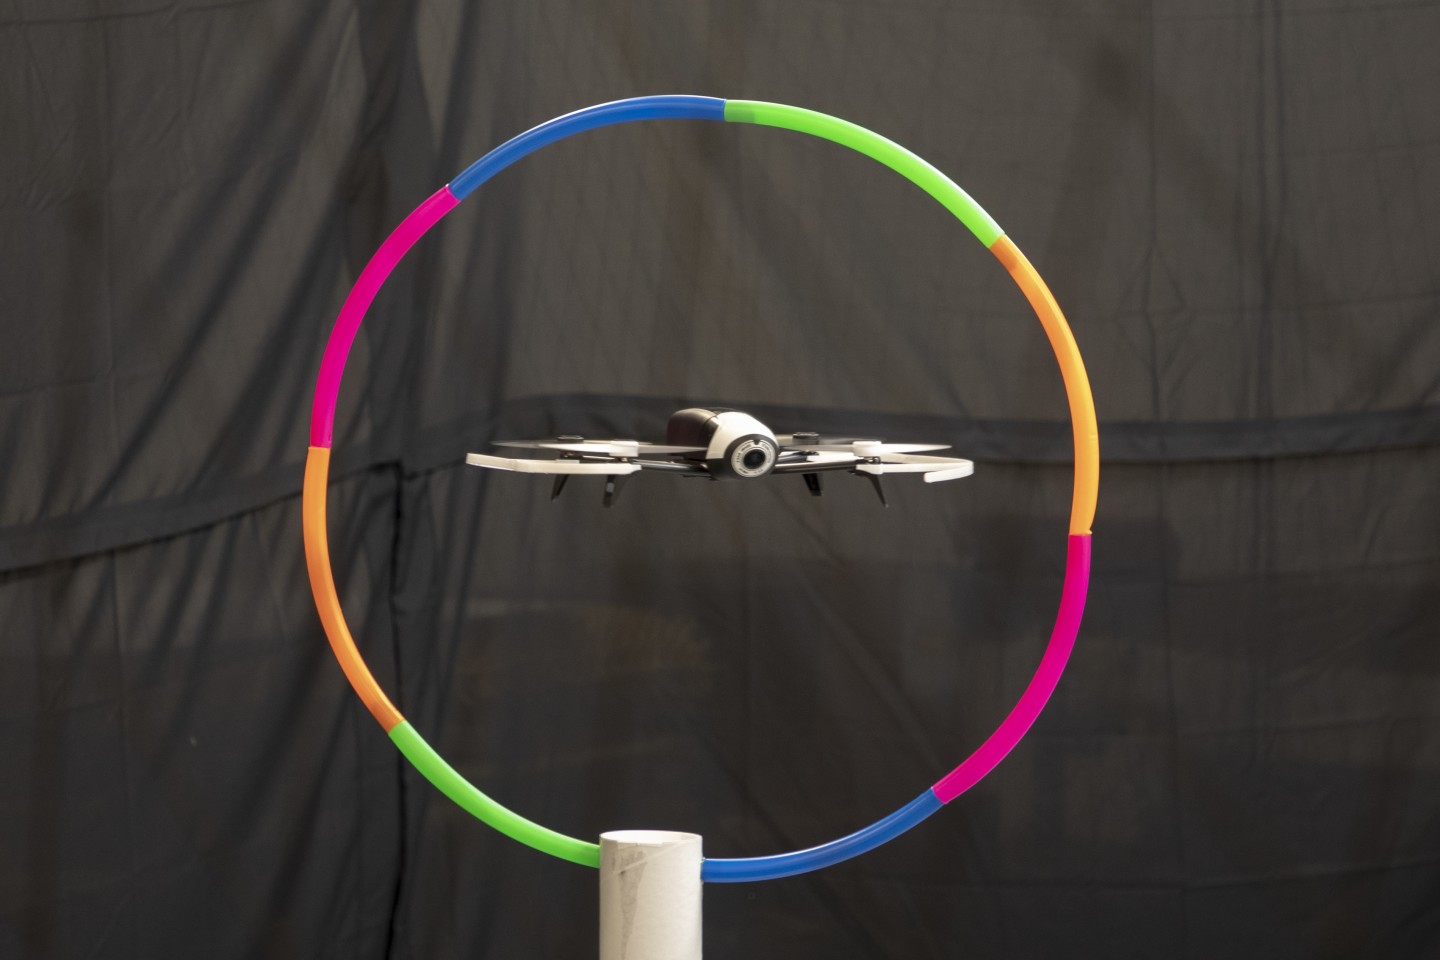
\includegraphics[width=\textwidth]{Images/Introduction/constrained_environment}
         \caption[Caption for LOF]{Quadrotor going though a loop.\protect\footnotemark[1]}
         \label{drone_hulahoop}
     \end{subfigure}
        \caption{Representation of the issues to be tackled in this master thesis.}
        \label{fig:three graphs}
\end{figure}

\footnotetext[1]{\url{https://newatlas.com/drones/muscle-signals-drone-control/\#gallery:2}, accessed on 01/08/2021.}

\pagebreak

\section*{Outline of the work}

The rest of the bibliography is structured as follows:


\begin{itemize}
\setlength{\itemindent}{-.5in}
	\item [] \textbf{Chapter 1} is devoted to introduce the system modeling of quadrotors. Specifically, a simplified dynamic model of the quadrotor will be presented by using Euler-Lagrange formalism. Then, moving on from the simple dynamic model, a more detailed dynamic model will be presented by using the Newton-Euler formalism. Finally, the state-space model of the quadrotor will be derived.

	\item [] \textbf{Chapter 2} provides an overview of state of the art in quadrotor control in addition to introducing the different potential control methods that can be used during the master thesis in order to properly control the quadrotor. 

	\item [] \textbf{Chapter 3} provides detailed explanations of how multi-flip maneuvers can be handled. Then, the link between a quadrotor performing a flip and a parallel robot crossing a singularity will be explained. In the end, a literature review is provided in order to show how the problem is tackled by different researches.

	\item [] \textbf{Chapter 4} is devoted to trajectory optimization. By using trajectory optimization, it will be possible to create feasible trajectories for quadrotors to perform the aggressive maneuvers in constrained environments.
	
\end{itemize}

\newpage

\chapter{System Modeling}

The principal objective of this chapter is to demonstrate the dynamic model of the quadrotor. In this case, both the Euler-Lagrange and the Newton-Euler formalism are used for expressing the mathematical and physical model of the quadrotor platform. However, the notion of position and orientation will be explained first. The lecture notes of Dr. Fantoni is considered as the reference \cite{Fantoni2016}.


After that, the derivation of the state space model which will be coded on the controller of the quadrotor is performed \cite{Bouabdalla2007}.



\begin{comment}
\section{Concepts and Generalities}
The dynamic model of the quadrotor will be derived based on the following assumptions:

\begin{itemize}
	\item The quadrotor has a rigid structure.
	\item The quadrotor has a symmetrical structure.
	\item The center of gravity (CoG) and the fixed frame at the center of the body are assumed to be coincident.
	\item The propellers of the quadrotor are assumed to be rigid.
	\item The thrust and drag forces are assumed to be proportional to the square of the spinning speed of each propeller.
\end{itemize}
 
The helicopter is a complex mechanical system, it gathers many physical effects from the domain of mechanics and aerodynamics \cite{houston_2001}. Thus, all the significant effects including the gyroscopic effects must be considered in the modeling of the quadrotor. A small list of the most important effects that a helicopter is subject to \cite{Mullhaupt1999} are briefly described in table \ref{physical_effects}:

\begin{table}[h]
\caption{The main physical effects that the helicopter is subject to. }\label{physical_effects}
\centering
\setlength{\tabcolsep}{10pt} % Default value: 6pt
\renewcommand{\arraystretch}{1} % Default value: 1
\begin{tabular}{c c c}
\hline
\hline
Effect & Source & formulation \\
\hline
Aerodynamic effects & \shortstack{Rotation of propeller \\ Flapping of blades} & $C \Omega^2$\\
\hline
Inertial counter torques & \shortstack{Change in propeller \\ spinning speed} & $ J \dot{\Omega}$\\
Gravitational effect & Position of the center of mass & {} \\
\hline
Gyroscopic effects & \shortstack{Orientation change  \\ of the rigid body} & $ I \theta \psi$\\
 {} & \shortstack{Orientation change  \\ of the propeller plane} & $ J \Omega_r \theta,\phi$ \\
 \hline
Friction & All helicopter motions & $C \dot{\phi},\dot{\theta},\dot{\psi}$\\
\hline
\hline
\end{tabular}
\end{table}

\newpage 




 \section{Modeling with Euler-Lagrange Formalism} 
 The dynamics of the rotation of a simple quadrotor are modeled using the Euler-Lagrange Formalism in this section. A fixed frame $E$ for the world frame and body fixed frame $B$ for the quadrotor are considered as represented in figure \ref{coordinate_system_simple}. The orientation of the quadrotor frame in space is provided by a rotation $R$ from $B$ to $E$, where $R\in SO3$ is a $3 \times 3 $ rotation matrix.
 
 
 \begin{figure}[h]
 \centering
 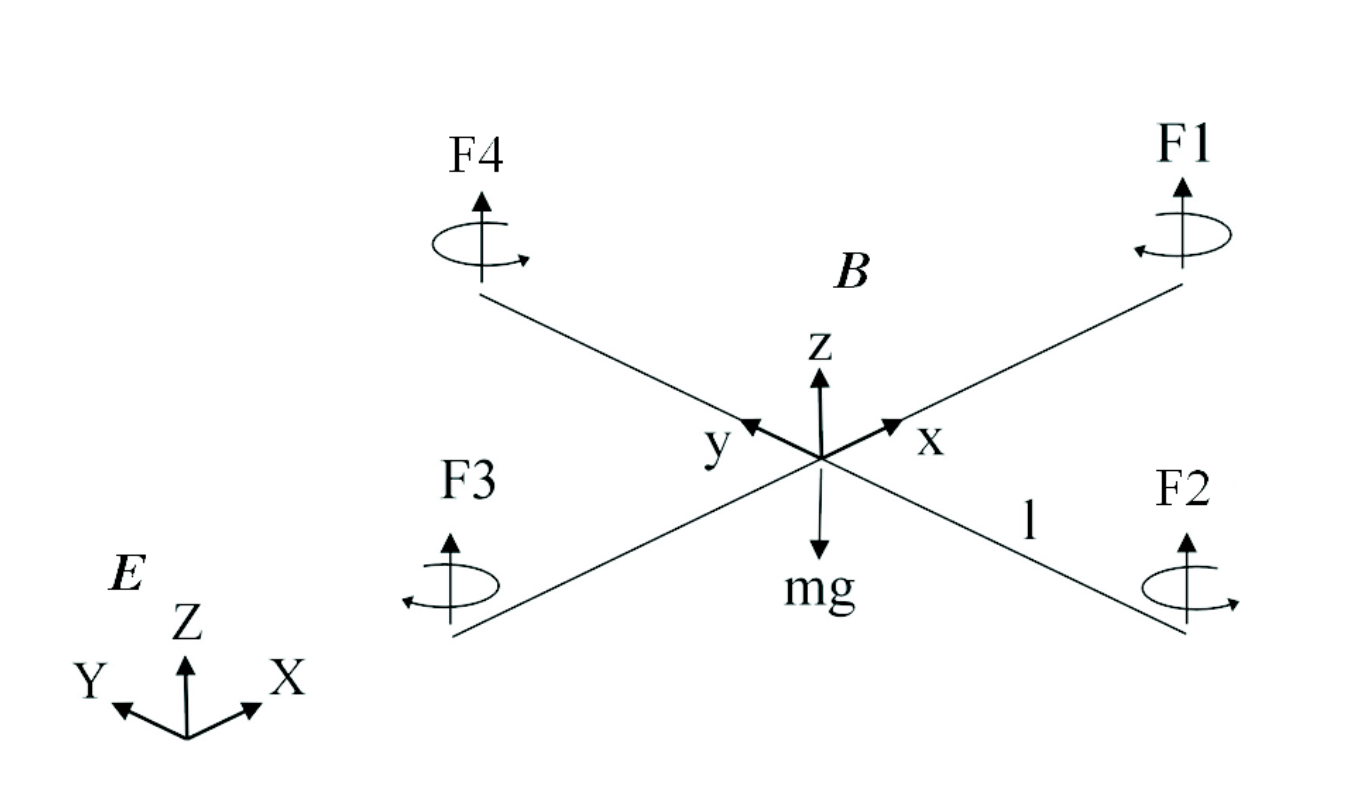
\includegraphics[width=0.5\textwidth]{Images/Modeling/Test_Bench}
 \caption{Simplified coordinate system of a quadrotor. \cite{Bouabdalla2007}}
 \label{coordinate_system_simple}
 \end{figure}

\subsection{Kinematics} 
 
 For any point of the body frame of the quadrotor expressed in the fixed world frame, the following can be written 
 ( c: $\cos$, s: $\sin$):   
 
 \begin{equation}\label{kinematics}
 \begin{cases}
 r_X= (c\psi c \theta ) x + ( c \psi s \theta s \phi  - s \psi c \phi) y + (c \psi s \theta c \phi + s \psi s \phi) z \\
 \\
 r_Y= (s\psi c \theta ) x + ( s \psi s \theta s \phi  + c \psi c \phi) y + (s \psi s \theta c \phi - c \psi s \phi) z \\
 \\
 r_Z= (-s \theta ) x + ( c \theta s \phi ) y + (c \theta c \phi) z \\ 
 \end{cases}
 \end{equation}

Thus, the velocities can be derived by differentiation (\ref{kinematics}), and the squared magnitude of the squared velocity can be expressed as follows for any point:

\begin{equation}\label{velocity_magnitude}
	v^2 = v_X^2 + v_Y^2 + v_Z^2\\
\end{equation} 

\subsection{Energy}

Assuming that the matrix of inertia is diagonal, then from equation (\ref{velocity_magnitude}), the expression of the kinetic energy can be calculated:

\begin{equation}\label{kinetic_energy}
T = \frac{1}{2} I_{xx}(\dot{\phi}-\dot{\psi} s \theta)^2 + \frac{1}{2} I_{yy}(\dot{\theta} c \phi + \dot{\psi} s \phi c \theta)^2 + \frac{1}{2} I_{zz}(\dot{\theta} s \phi - \dot{\psi} c \phi)^2
\end{equation}

Using the formula of the potential energy, equation (\ref{kinetic_energy}) can be expressed in the fixed world frame as: 

\begin{equation}\label{potential_energy}
V = \int xdm(x)(-g s \theta) + \int ydm(y)(g s \phi c \theta) + \int z dm (z) (g c \phi c \theta) 
\end{equation}

\newpage

\subsection{Equation of Motion}

By using the Euler-Lagrange formalism:


\begin{equation}
L = T - V \text{\hspace{0.5cm} ,\hspace{0.5cm}} \Gamma_i = \frac{d}{dt}\bigg(\frac{\partial L}{\partial \dot{q}_i}\bigg) - \frac{\partial L}{\partial q_i}
\end{equation}
 
 Where $L$, $\Gamma_i$ and $q_i$ are the Lagrangian, the generalized forces and the generalized coordinates respectively. Thus, the equations of motion can be expressed as follows: 
 
 \begin{equation}
 \begin{cases}
 I_{xx}\ddot{\phi} = \dot{\theta} \dot{\psi}(I_{yy}-I_{zz})\\
 \\
 I_{yy}\ddot{\theta} = \dot{\phi} \dot{\psi}(I_{zz}-I_{xx})\\
 \\
 I_{zz}\ddot{\psi} = \dot{\phi} \dot{\theta} (I_{xx} - I_{yy})
 \end{cases}
 \end{equation}
 
Moreover, the torques that are nonconservative and acting on the quadrotor, are due to two different causes. First, they are due to the thrust of each rotor pairs in figure \ref{coordinate_system_simple}:

\begin{equation}
\begin{cases}
\tau_x = bl(\Omega_4^2 - \Omega_2^2)\\
\\
\tau_y = bl(\Omega_3^2 - \Omega_1^2)\\
\\
\tau_z = bl(\Omega_1^2 - \Omega_2^2 + \Omega_3^2 - \Omega_4^2)\\
\end{cases}
\end{equation}

Second, they are also due to the gyroscopic effect which is the result of the rotation of the propellers:

\begin{equation}
\begin{cases}
\tau_x' = J_r \omega_y (\Omega_1 + \Omega_3 - \Omega_2 - \Omega_4)\\
\\
\tau_y' = J_r \omega_x (\Omega_2 + \Omega_4 - \Omega_1 - \Omega_3)\\
\end{cases}
\end{equation}

\subsection{The Derived Dynamic Model}

The dynamic model of the quadrotor which describes the rotations of roll, pitch and yaw consists of three terms:
\begin{enumerate}
	\item The actuator torques.
	\item The gyroscopic effects that are due to the rotation of the rigid body.
	\item The gyroscopic effects that are due to rotation of the propeller that is coupled with the rotation of the body.
\end{enumerate}

 Thus, the dynamic model of the quadrotor is:
 
 \begin{equation}\label{dynamic_model}
 	\begin{cases}
 		I_{xx}\ddot{\phi}= \dot{\theta}\dot{\psi}(I_{yy}-I_{zz})-J \dot{\theta} \Omega_r + \tau_x \\
 		\\
 		I_{yy}\ddot{\theta}= \dot{\theta}\dot{\psi}(I_{zz}-I_{xx})+J \dot{\phi} \Omega_r + \tau_y \\
 		\\
 		I_{zz}\ddot{\psi}= \dot{\phi}\dot{\theta}(I_{xx}-I_{yy}) + \tau_z \\	
 	\end{cases}
 \end{equation}

 
 
 \newpage
 
 \subsection{Rotor Dynamics}
 
 DC motors are used to drive the rotors of a quadrotor. So, the established equations of a DC motor are the following:

\begin{equation}\label{DC_motor_dynamics}
\begin{cases}
L \frac{di}{dt}=u - R_{mot}i - k_e \omega_m\\
\\
J_m \frac{d \omega_m}{dt} = \tau_m - \tau_d \\
\end{cases}
\end{equation} 

Since small motors are used in which they also have little inductance, then the second order equation of the DC motor dynamics is given by:

\begin{equation}\label{DC_motor_2nd_order_dynamics_first}
	J_m \frac{d\omega_m}{dt} = -\frac{k_m^2}{R_{mot}}\omega_m - \tau_d + \frac{k_m}{R_{mot}}u
\end{equation}
 
When the gearbox and the propeller models are introduced, then equation (\ref{DC_motor_2nd_order_dynamics_first}) becomes:

\begin{equation}\label{DC_motor_2nd_order_dynamics}
\begin{cases}
	\dot{\omega}_m = - \frac{1}{\tau}\omega_m - \frac{d}{\eta r^3 J_t}\omega_m^2 + \frac{1}{k_m \tau}u\\
	\\
	\frac{1}{\tau} = \frac{k_m^2}{RJ_t}\\
	\end{cases}
\end{equation}
 
Moreover, linearization of equation (\ref{DC_motor_2nd_order_dynamics}) can be done around an operation point $\dot{\omega}_0$ to the form $\dot{\omega}_m = -A \omega_m + B u + C$ with: 

\begin{equation}
A = \bigg( \frac{1}{\tau}+\frac{2d\omega_0}{\eta r^3 J_t} \bigg) \text{ \hfill , \hfill} B = \bigg( \frac{1}{k_m \tau} \bigg) \text{\hfill , \hfill} C = \bigg( \frac{d \omega_0^2}{\eta r^3 J_t} \bigg)
\end{equation}
 
 
 \section{Modeling with Newton-Euler Formalism}
 
The model above was derived in succession as shown in papers  \cite{Bouabdallah2004,Bouabdallah2005a,Bouabdallah2005b} . The dynamic equations below include rolling moments $R_m$, hub forces $H$ and various aerodynamic effects.
Thus, this is a more realistic dynamic model, especially when the quadrotor flies in a forward manner. 
With the previous versions of the dynamic model, it was required to moderately tune the control parameters in order to have experiments that are successful.

The dynamic model expressed in the Newton-Euler formalism of a rigid body that is subject to external forces acting on the center of mass  \cite{Murray1994} is expressed as follows:

\begin{equation}\label{NE_Formalism}
\begin{bmatrix}
m I_{3 \times 3} && 0 \\
0 && I \\
\end{bmatrix}
\begin{bmatrix}
\dot{V}\\
\dot{\omega}\\
\end{bmatrix}
+ \begin{bmatrix}
\omega \times mV \\
\omega \times I \omega \\
\end{bmatrix}
=
\begin{bmatrix}
F \\
\tau \\
\end{bmatrix}
\end{equation}
 
Considering a fixed world frame $E$ and a fixed body frame $B$ on the quadrotor as shown in figure \ref{coordinate_system_detailed_quadrotor}. Then, by the use of the Euler angles, the orientation of the rigid body of the quadrotor in space is expressed by a rotation $R$ from $B$ to $E$, where $R \in SO3$ is a rotation matrix. 
 
 \begin{figure}[h]
\centering
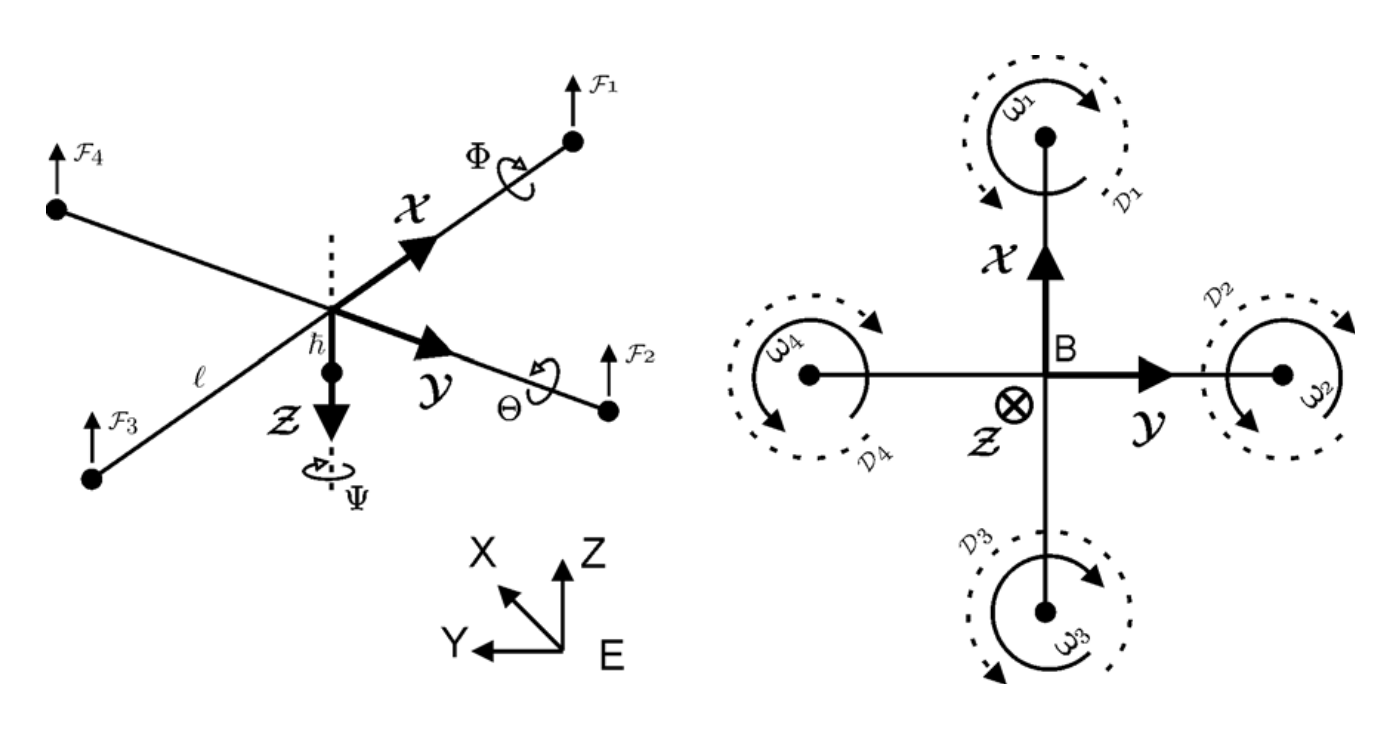
\includegraphics[width=0.5\textwidth]{Images/Modeling/Detailed_quadrotor}
\caption{Detailed coordinate system showing the forces with the roll, pitch and yaw angles (left) and the moments (right) applied on a quadrotor. \cite{Bouabdalla2007}}
\label{coordinate_system_detailed_quadrotor}
\end{figure}
 
\newpage

\subsection{Aerodynamic Forces and Moments}

The aerodynamic forces and moments are computed using a mix of blade element and momentum theory \cite{Leishmana}. This is based off of the work of Gary Fay during the project of the Mesicopter \cite{Leishmanb}. For a simpler readings of the equations provided below, some symbols are recalled:

\begin{table}[h]
\centering
\setlength{\tabcolsep}{10pt} % Default value: 6pt
\renewcommand{\arraystretch}{1} % Default
\begin{tabular}{l l}
$\sigma$: solidity ration & $\lambda$: inflow ratio \\
$a$: lift slope & $v$: induced velocity \\
$\mu$: rotor advance ration & $\rho$: air density

\end{tabular}
\captionsetup[table]{list=no}
\end{table}
 
\subsubsection*{Thrust Force}

The thrust force is due to all the vertical forces that the blade elements are subject to.

\begin{equation}\label{thrust_force}
\begin{cases}
T = C_T \rho A(\Omega R_{rad})^2\\
\\
\frac{C_T}{\sigma a} = (\frac{1}{6} + \frac{1}{4} \mu^2)\theta_0 - (1+\mu^2)\frac{\theta_{tw}}{8} - \frac{1}{5} \lambda \\
\end{cases}
\end{equation}

\subsubsection*{Hub Force}

The hub force is due to all the horizontal forces that the blade elements are subject to.

\begin{equation}
\begin{cases}
H = C_H \rho A(\Omega R_{rad})^2\\
\\
\frac{C_H}{\sigma a} = (\frac{1}{4a} \mu \overline{C_d} + \frac{1}{4} \lambda \mu (\theta_0 - \frac{\theta_{tw}}{2})\\
\end{cases}
\end{equation}

\subsubsection*{Drag Moment}

The drag moment about the rotor shaft is due to the aerodynamic forces that the blade elements are subject to. The horizontal forces that are acting on the rotor are multiplied by the moment arm and  integrated over the rotor. The drag moment gives the required power to spin the rotor.

\begin{equation}
\begin{cases}
	Q = C_Q \rho A (\Omega R_{rad})^2 R_{rad}\\
	\\
	\frac{C_Q}{\sigma a} = \frac{1}{8a}(1+\mu^2) \overline{C_d} + \lambda (\frac{1}{6} \theta_0 - \frac{1}{8} \theta_{tw} - \frac{1}{4} \lambda)
\end{cases}
\end{equation}

\newpage

\subsubsection*{Rolling moment}


The rolling moment of a propeller occurs when the blade that is advancing is producing more lift than the blade that is retreating in forwarding flight. It is the integration of the lift of every single section that is acting at a given radius over the entire rotor.
The reader should notice that the rolling moment is not the same as the propeller radius, or the overall rolling moment which is due to other effects or the rotation matrix $R$. So, there should not be any confusion.

\begin{equation}
\begin{cases}
R_m = C_{R_m}\rho A (\Omega R_{rad})^2 R_{rad} \\
\\
\frac{C_{R_m}}{\sigma a} = -\mu (\frac{1}{6} \theta_0 - \frac{1}{8} \theta_{tw} - \frac{1}{8} \lambda)\\
\end{cases}
\end{equation}

\subsubsection*{Ground Effect}


When operating near the ground (at a height equivalent to half the diameter of the rotor), helicopters experience thrust augmentation which is caused by greater efficiency of the rotor. This is linked to a decrease in the velocity of induced airflow. Moreover, this is called Ground Effect. Different approaches to deal with this effect can be found in literature, for example, adaptive techniques can  be used \cite{Guenard2006}.
However, the objective is to find a model that is simple and mainly captures the change in the velocity of the induced inflow.
Cheeseman \cite{Cheeseman1957} states (reached from the images method \cite{Griffiths2002}) that if the power is constant ($T_{OGE}v_{i,OGE} = T_{IGE}v_{i,IGE}$), the generated velocity at the center of the rotor by its image is $\delta v_i = Av_i/16 \pi z^2$.
Cheesman acquired the relation (\ref{Cheeseman}) by using the assumption that both $v_i$ and $\delta v_i$ are constant over the disk, which results in $v_{i,IGE}=v_i-\delta v_i$.

\begin{equation}\label{Cheeseman}
\frac{T_{IGE}}{T_{OGE}}=\frac{1}{1-\frac{R^2_{rad}}{16 z^2}}
\end{equation}

An alternative way to move forward is to consider that the inflow ratio of the inflow ratio is $\lambda_{IGE} = (v_{i,OGE}-\delta v_i - \dot{z})/\Omega R_{rad}$, where the change of the velocity of the induced inflow is $\delta v_i = v_i/(4z/R_{rad})^2$. Then, the thrust coefficient (\ref{thrust_force}) IGE can be rewritten  as:

\begin{equation}
\begin{cases}
T_{IGE}=C_T^{IGE} \rho A(\Omega R_{rad})^2 \\
\\
\frac{C_T^{IGE}}{\sigma a} = \frac{C_T^{OGE}}{\sigma a} + \frac{\delta v_i}{4 \Omega R_{rad}}\\
\end{cases}
\end{equation} 


\newpage

\subsection{General Moments and Forces}\label{forces_and_moments}

The motion of the quadrotor is the result of several forces and moments that are originating from different physical effects \cite{Bouabdalla2007}. In this model, the following effects are considered (with $c$: $\cos$, $s$:$\sin$).

\subsubsection*{Rolling Moments}

\setlength{\tabcolsep}{20pt}
 \begin{tabular}{lp{0.8\textwidth}}
  body gyro effect & $\dot{\theta}\dot{\psi}(I_{yy}-I_{zz})$\\
  \\
  propeller gyro effect & $J_r \dot{\theta}\Omega_r$\\
  \\
  pitch actuators action & $l(-T_2+T_4)$\\
  \\
  hub moment due to forward flight & $h(\sum_{i=1}^4 H_{yi})$\\
  \\
  rolling moment due to forward flight & $(-1)^{i+1}\sum_{i=1}^4 R_{mxi}$\\
  \\
\end{tabular}

\subsubsection*{Pitching Moments}

\setlength{\tabcolsep}{20pt}
 \begin{tabular}{lp{0.8\textwidth}}
 body gyro effect & $\dot{\phi}\dot{\psi}(I_{zz}-I_{xx})$\\
 \\
 propeller gyro effect & $J_r \dot{\phi}\Omega_r$ \\
 \\
 pitch actuators action & $l(T_1-T_3)$\\
 \\
 hub moment due to forward flight & $h(\sum_{i=1}^4 H_{xi})$\\
 \\
 rolling moment due to side-ward flight &  $(-1)^{i+1}\sum_{i=1}^4 R_{myi}$\\
\end{tabular}

\subsubsection*{Yawing Moments}

\setlength{\tabcolsep}{20pt}
 \begin{tabular}{lp{0.8\textwidth}}
body gyro effect & $\dot{\theta}\dot{\phi}(I_{xx}-I_{yy})$\\
\\
inertial counter-torque & $J_r \dot{\Omega}_r$\\
\\
counter-torque unbalance & $(-1)^i\sum_{i=1}^4 Q_i$\\
\\
hub force unbalance in forward flight & $l(H_{x2}-H_{x4})$ \\
\\
hub force unbalance in sideward flight & $l(-H_{y1}+H_{y3})$\\

\end{tabular}


\subsubsection*{Forces Along z Axis}

%
\setlength{\tabcolsep}{58pt}
 \begin{tabular}{lp{1\textwidth}}
actuators action & $c \psi c \phi (\sum_{i=1}^4T_i$\\
\\
weight & $mg$ \\

\end{tabular}

\subsubsection*{Forces Along x Axis}
\setlength{\tabcolsep}{58pt}
 \begin{tabular}{lp{1\textwidth}}
actuators action & $ (s \psi s \phi + c \psi s \theta c \phi)(\sum_{i=1}^4 T_i) $\\
\\
hub force in x axis & $-\sum_{i=1}^4 H_{xi}$ \\
\\
friction & $\frac{1}{2}C_x A_c \rho \dot{x}|\dot{x}|$

\end{tabular}


\subsubsection*{Forces Along y Axis}
\setlength{\tabcolsep}{58pt}
 \begin{tabular}{lp{1\textwidth}}
actuators action & $ (-c \psi s \phi + s \psi s \theta c \phi)(\sum_{i=1}^4 T_i) $\\
\\
hub force in y axis & $-\sum_{i=1}^4 H_{yi}$ \\
\\
friction & $\frac{1}{2}C_y A_c \rho \dot{y}|\dot{y}|$

\end{tabular}

\subsection{Equations of Motion}\label{detail_equation_of_motion}

The equations of motion are derived from (\ref{NE_Formalism}) in addition to all the forces and the moments that were listed in subsection \ref{forces_and_moments}.

\begin{equation}\label{detailed_dynamic_model}
\begin{cases}
I_{xx}\ddot{\phi} = \dot{\theta} \dot{\psi}(I_{yy}-I_{zz}) + J_r \dot{\theta}\Omega_r + l(-T_2+T_4)-h(\sum_{i=1}^4H_{yi})+(-1)^{i+1} \sum_{i=1}^4 R_{mxi}\\
\\
I_{yy}\ddot{\theta} = \dot{\phi} \dot{\psi}(I_{zz}-I_{xx}) - J_r \dot{\phi}\Omega_r + l(T_1-T_3) + h(\sum_{i=1}^4H_{xi})+(-1)^{i+1} \sum_{i=1}^4 R_{mxi}\\
\\
I_{zz}\ddot{\psi} = \dot{\phi} \dot{\psi}(I_{xx}-I_{yy}) + J_r \dot{\Omega}_r +(-1)^i \sum_{i=1}^4 Q_i + l(H_{x2}-H_{x4})+l(-H_{y1}+H_{y3})\\
\\
m\ddot{z} = mg -(c \psi c \phi)\sum_{i=1}^4T_i\\
\\
m\ddot{x} = (s \psi s \phi + c \psi s \theta c \phi) \sum_{i=1}^4 T_i - \sum_{i=1}^4 H_{xi}-\frac{1}{2}C_xA_c \rho \dot{x}|\dot{x}|\\
\\
m \ddot{y} = ( - c \psi s \phi + s \psi s \theta c \phi) \sum_{i=1}^4 T_i - \sum_{i=1}^4H_{yi} - \frac{1}{2}C_y A_c \rho \dot{y}|\dot{y}|\\
\end{cases}
\end{equation}

\newpage

\end{comment}


\section{Notion of Position and Orientation}

The configuration of a vehicle, namely the \textit{pose}, includes the parameters that pertmits to describe the mobile frame $R_M$ with respect to the working frame $R_O$. In addition, there are several methods to describe the rotation of a rigid body in space, for instance, Euler angles, Cardan angles, etc. \cite{Goldstein1980}. The main distinction between the Euler angles and the Cardan angles is that Cardan angles express rotations around three different axes (e.g. $x-y-z$, or $x-y'' -z''$), whereas Euler angles utilize the same axis for both the first and third elemental rotations(e.g., $z-x-z$, or $z-x'-z''$)

A common representation of the pose of a vehicle in 3D Euclidean space is the following:



\begin{equation}
q=[\begin{array}{c c c c c c }
x & y & z & \psi & \theta & \phi
\end{array}]^{\intercal}
\end{equation}

The pose can be described as the transformation from the working frame related to the environment $R_O$ to the mobile frame $R_M$ based on the four following procedures \cite{Fantoni2016}:

\begin{itemize}
	\item The translation $\overrightarrow{OM}$ from $R_O$ to $R_M$: $(M,\overrightarrow{s_0}, \overrightarrow{n_0}, \overrightarrow{a_0} )$.
	\item The rotation $(\psi, \overrightarrow{a_0})$ where $\psi$ is the yaw angle from $R_O(M,\overrightarrow{s_0}, \overrightarrow{n_0}, \overrightarrow{a_0} )$ to $R_1(M,\overrightarrow{s_1}, \overrightarrow{n_1}, \overrightarrow{a_0} )$.
	\item The rotation $(\theta, \overrightarrow{n_1})$ where $\theta$ is the pitch angle from $R_1$ to $R_2 (M,\overrightarrow{s_2}, \overrightarrow{n_1}, \overrightarrow{a_1} )$.
	\item The rotation $(\phi, \overrightarrow{s_2})$ where $\phi$ is the roll angle from $R_2$ to $R_M (M,\overrightarrow{s_2}, \overrightarrow{n_2}, \overrightarrow{a_2} ) = R_M$ 
\end{itemize}



\newpage

\begin{figure}[h]
\centering
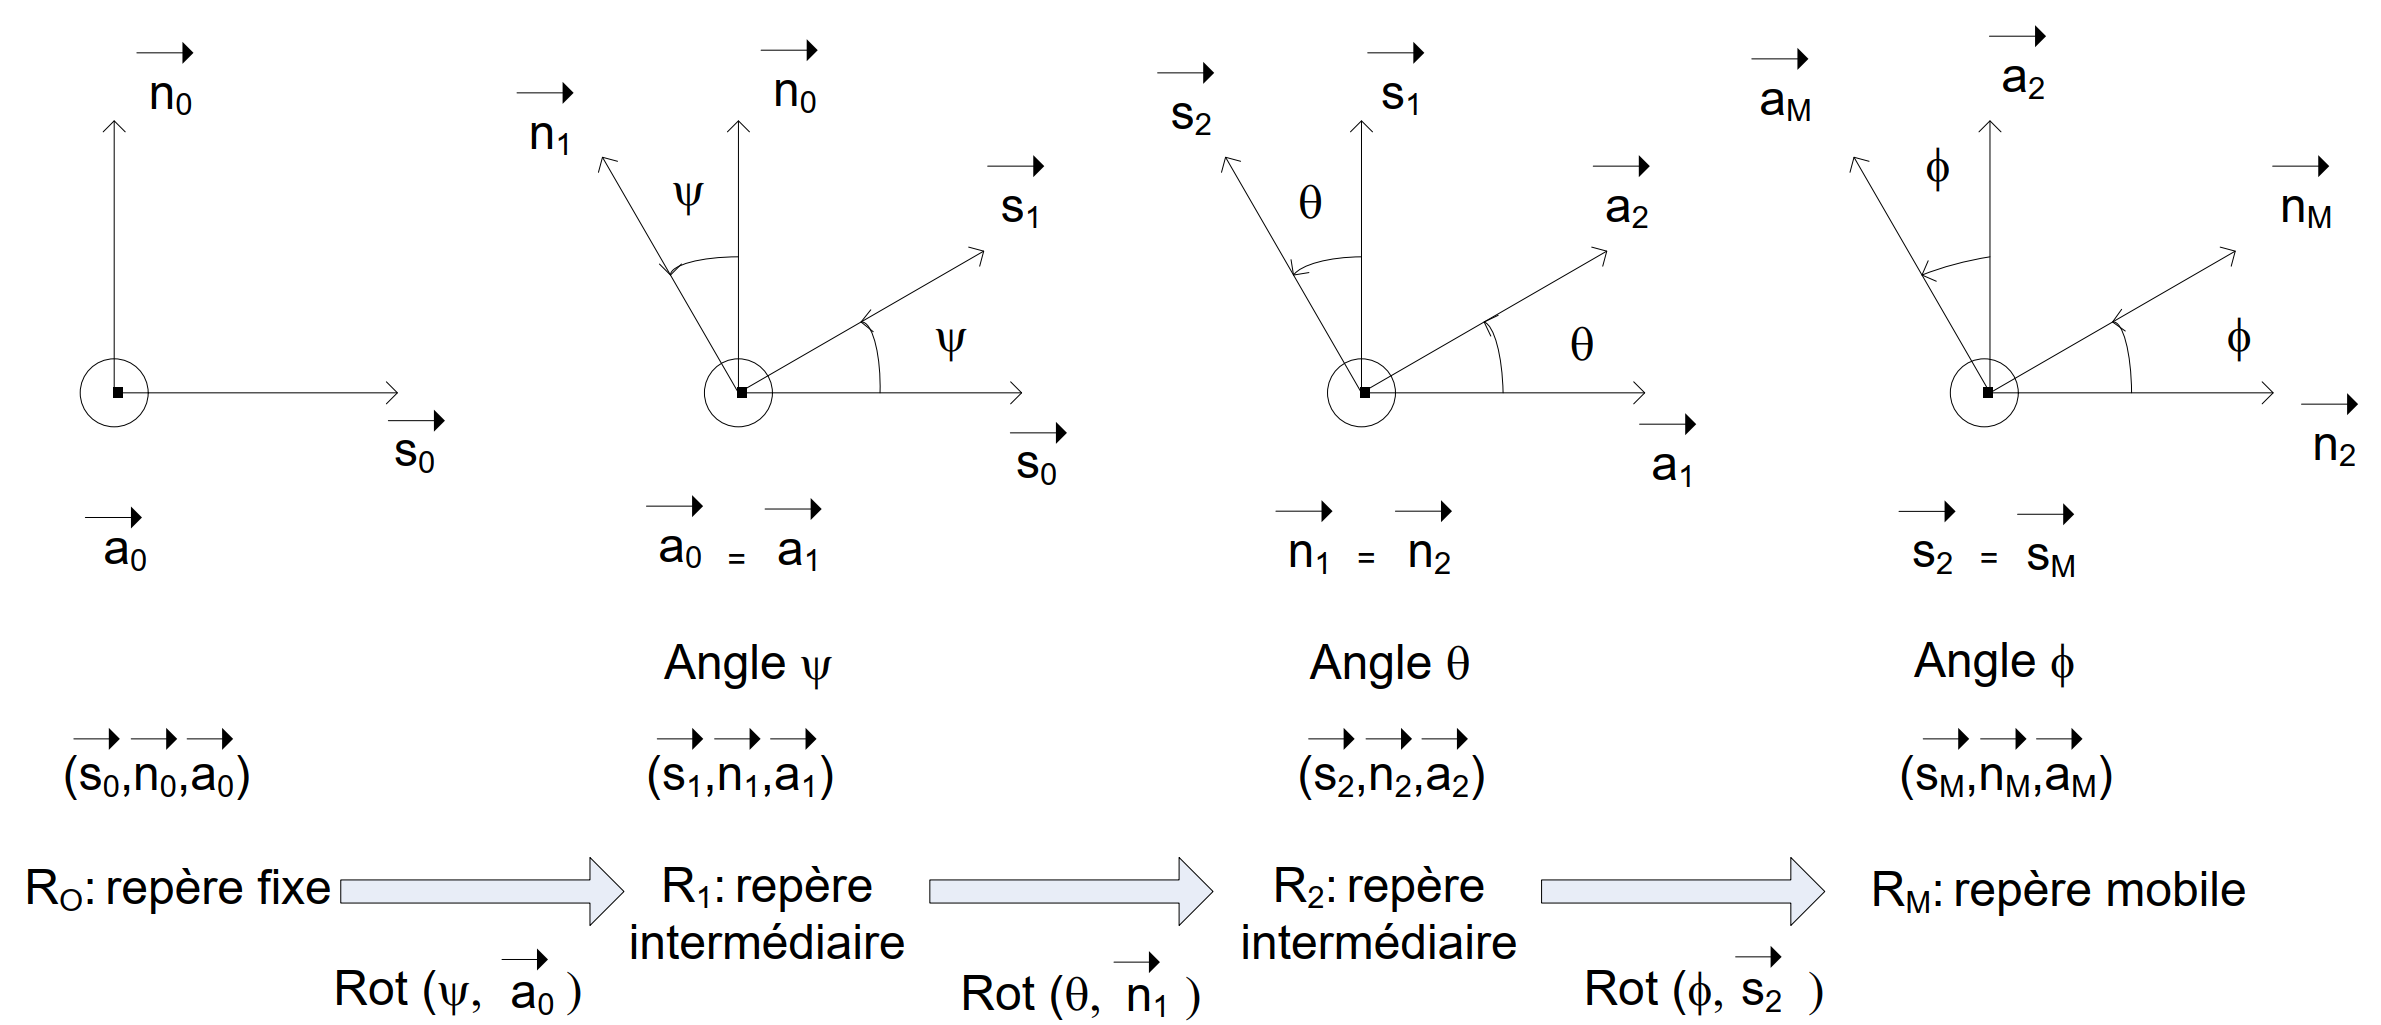
\includegraphics[width=\textwidth]{Images/Modeling/Fantoni_d}
\caption{Representation of the Euler Transformations \cite{Fantoni2016} }
\label{Fantoni_d}
\end{figure}

The related change of coordinates matrices are expressed as follows:


\begin{equation}
	L = {}^{O}A_1 = Rot(\psi, \overrightarrow{a_0}) = \begin{bmatrix}
	\cos \psi && - \sin \psi && 0 \\
	\sin \psi && \cos \psi && 0 \\
	0 && 0 && 1 
	\end{bmatrix}
\end{equation}

\begin{equation}
	T = {}^{1}A_2 = Rot(\theta, \overrightarrow{n_1}) = \begin{bmatrix}
	\cos \theta && 0 && \sin \theta \\
	0 && 1 && 0 \\
	- \sin \theta && 0 && \cos \theta 
	\end{bmatrix}
\end{equation}

\begin{equation}
	R = {}^{2}A_M = Rot(\phi, \overrightarrow{s_2}) = \begin{bmatrix}
	1 && 0 && 0 \\
	0 && \cos \phi && - \sin \phi \\
	0 && \sin \phi && \cos \phi 
	\end{bmatrix}
\end{equation}

with $L, T$ and $R$ denoting rotation matrices of roll, pitch and yaw respectively.
Hereafter, $Rot(\psi, \overrightarrow{a_0})$, $Rot(\theta, \overrightarrow{n_1})$ and $Rot(\phi, \overrightarrow{s_2})$ will denote the corresponding change of coordinate matrices.

Thus, the transition matrix from the mobile frame to the fixed frame is then expressed as follows: 

\begin{align}
	LTR &= {}^{O}A_M = Rot(\psi, \overrightarrow{a_0}) Rot(\theta, \overrightarrow{n_1}) Rot(\phi, \overrightarrow{s_2}) \nonumber \\
	&= \begin{bmatrix}
	\cos \psi \cos \theta && - \sin \psi \cos \phi + \cos \psi \sin \theta \sin \phi && \sin \psi \sin \theta + \cos \psi \sin \theta \cos \phi \\
	\cos \theta \sin \psi && \cos \psi \cos \phi + \sin \psi \sin \theta \sin \phi && - \sin \phi \cos \psi + \sin \psi \sin \theta \cos \phi \\
	-\sin \theta && \cos \theta \sin \phi && \cos \theta \cos \phi
	\end{bmatrix}
\end{align}





\newpage


\section{Inputs}

The principal forces and torques that the quadrotor is subject to, are generated by the rotations of the propellers. 

\paragraph{The forces} The forces that are acting on the quadrotor are the weight and the consequent lift which is created by the 4 rotors:

\begin{equation}
\overrightarrow{F_{\xi}}= \overrightarrow{P} + \sum \overrightarrow{f_i}
\end{equation} 

with the weight is expressed as 
$ \overrightarrow{P}= \begin{bmatrix}
0 \\ 
0 \\
-mg \\
\end{bmatrix}$

And, $\overrightarrow{f_{i}}$ is the lift resulting from every individual motor $M_i$ given that the motors $M_1$ and $M_3$ are rotating in the counter-clockwise direction and the motors $M_2$ and $M_4$ are rotating in the clockwise direction. So, $\overrightarrow{f_i}$ is expressed as $\overrightarrow{f_i}=\begin{bmatrix}
0 \\ 
0 \\
f_i \\
\end{bmatrix}=b \begin{bmatrix}
0 \\ 
0 \\
\omega_i^2 \\
\end{bmatrix} $  

$f_i = b \omega^2; i=1,\ldots,4$\\
$\omega_i$: rotational velocity of every motor $M_i$\\
$b$: Thrust coefficient\\

The consequent lift is the full thrust of the UAV and is expressed by $u=\sum \overrightarrow{f_i}$. It is lying on the same line as the $u_z$ axis of the $R_U$ frame where the final expression of $\overrightarrow{F_{\xi}}$ is made of two parts . The first part (the weight)  is expressed in the fixed frame and the second part (the total thrust $u$) is expressed in the mobile frame: 

\begin{equation}
\overrightarrow{F_{\xi}}  = \begin{bmatrix}
0 \\
0 \\
-mg \\
\end{bmatrix} 
+ 
b \begin{bmatrix}
0 \\ 
0 \\
\omega_1^2 + \omega_2^2 + \omega_3^2 + \omega_4^2\\
\end{bmatrix}=
\prescript{O}{}{\begin{bmatrix}
0 \\
0 \\
-mg \\
\end{bmatrix}}
+ b \prescript{U}{}{\begin{bmatrix}
0 \\ 
0 \\
\omega_1^2 + \omega_2^2 + \omega_3^2 + \omega_4^2\\
\end{bmatrix}}
\end{equation}








\newpage

\paragraph{The torques}
Regarding the torques, they are also divided into two parts. The first part is the result of the relations between the velocities of the rotors. Whereas the other part is generated by the gyroscopic effects that are resulting from the change of attitude direction of the rotors. In fact, a rotation around the $u_x$ or $u_y$ axis coupled to the rotation of the rotors that is executed around the $u_z$ axis, generates a torque respectively on $u_x$ or $u_y$ axis.

By taking $\tau=\begin{bmatrix}
\tau_1 && \tau_2 && \tau_3 
\end{bmatrix}^{\intercal}$ to be the consequent torque of the quadrotor. It is divided into two parts, namely $\tau_a$ which contains the rotation torques (roll,pitch and yaw) on the 3 axes ($\tau_{\phi}, \tau_{\theta}, \tau_{\psi}$) and the torque $\tau_G$ which is the result of the gyroscopic effects of the rotors, which is usually neglected in many works.

\begin{equation}
	\tau = \tau_a + \tau_G
\end{equation}

with:

\begin{itemize}
	\item $\tau_a = \begin{bmatrix}
\tau_{\phi}\\
\tau_{\theta}\\
\tau_{\psi}\\
\end{bmatrix}= \begin{bmatrix}
l(f_4 - f_2)\\
l(f_3 - f_1)\\
\sum \tau_{M_i}\\
\end{bmatrix}$\\
$\sum \tau_{M_i} = \sum d \omega_i^2=d(\omega_1^2-\omega_2^2+\omega_3^2-\omega_4^2); i=1,\ldots 4$: motor torque about the axis.\\
$d$: drag coefficient .\\
$l$: distance between the center of gravity (CoG) of the quadrotor and the axis of motor $M_i$.

	\item $\tau_G=\overrightarrow{\omega}\times J_r \begin{bmatrix}
0 \\
0 \\
\omega_1 - \omega_2 + \omega_3 - \omega_4 \\
\end{bmatrix} = \begin{bmatrix}
-q J_r (\omega_1 - \omega_2 + \omega_3 - \omega_4)\\
p J_r (\omega_1 - \omega_2 + \omega_3 - \omega_4)\\
0 \\
\end{bmatrix}$

$\overrightarrow{\omega} = \begin{bmatrix}
p \\
q \\
r \\
\end{bmatrix}$: angular velocities.
$\omega_i$: spinning speeds of motors $M_i$.
$J_r$: rotor inertia.
\end{itemize}

Thus, the total torque $\tau$ is expressed as follows:

\begin{equation}\label{total_torque_equation}
\tau = \begin{bmatrix}
\tau_1\\
\tau_2\\
\tau_3\\
\end{bmatrix} = \tau_a + \tau_G = \begin{bmatrix}
l(f_4-f_2) - qJ_r(\omega_1-\omega_2+\omega_3-\omega_4)\\
l(f_3-f_1) + pJ_r(\omega_1-\omega_2+\omega_3-\omega_4)\\
d(\omega_1^2-\omega_2^2+\omega_3^2-\omega_4^2)\\
\end{bmatrix}
\end{equation}

\subsubsection*{System Inputs}

Thus, there exists two types of forces and torques that are acting on the quadrotor platform: the translation force $F_{\xi}$ which is called the thrust $u$, and the torque $\tau$ which represents all the torques about the distinct axes ($\tau_{\phi}, \tau_{\theta}, \tau_{\psi} $). \\
Rather than controling the velocities of the motors, the control in torque and thrust is synthesized, from which motor velocities are effortlessly inferred. Thus, the quadrotor has four control inputs, which are the inputs of its motors:

\begin{align*}
u_1 &= u \text{ (thrust)} \\
u_2 &= \tau_{\phi}\\
u_3 &= \tau_{\theta}\\
u_4 &= \tau_{\psi}\\
\end{align*}

The various torques and forces which are taken into account in this study are illustrated in figure \ref{Fantoni_a}.

\newpage

\section{Dynamical equations}

The dynamics equations of motion of a mechanism can be expressed by using either the Euler-Lagrange formalism or the Newton-Euler formalism.

\begin{figure}[h]
\centering
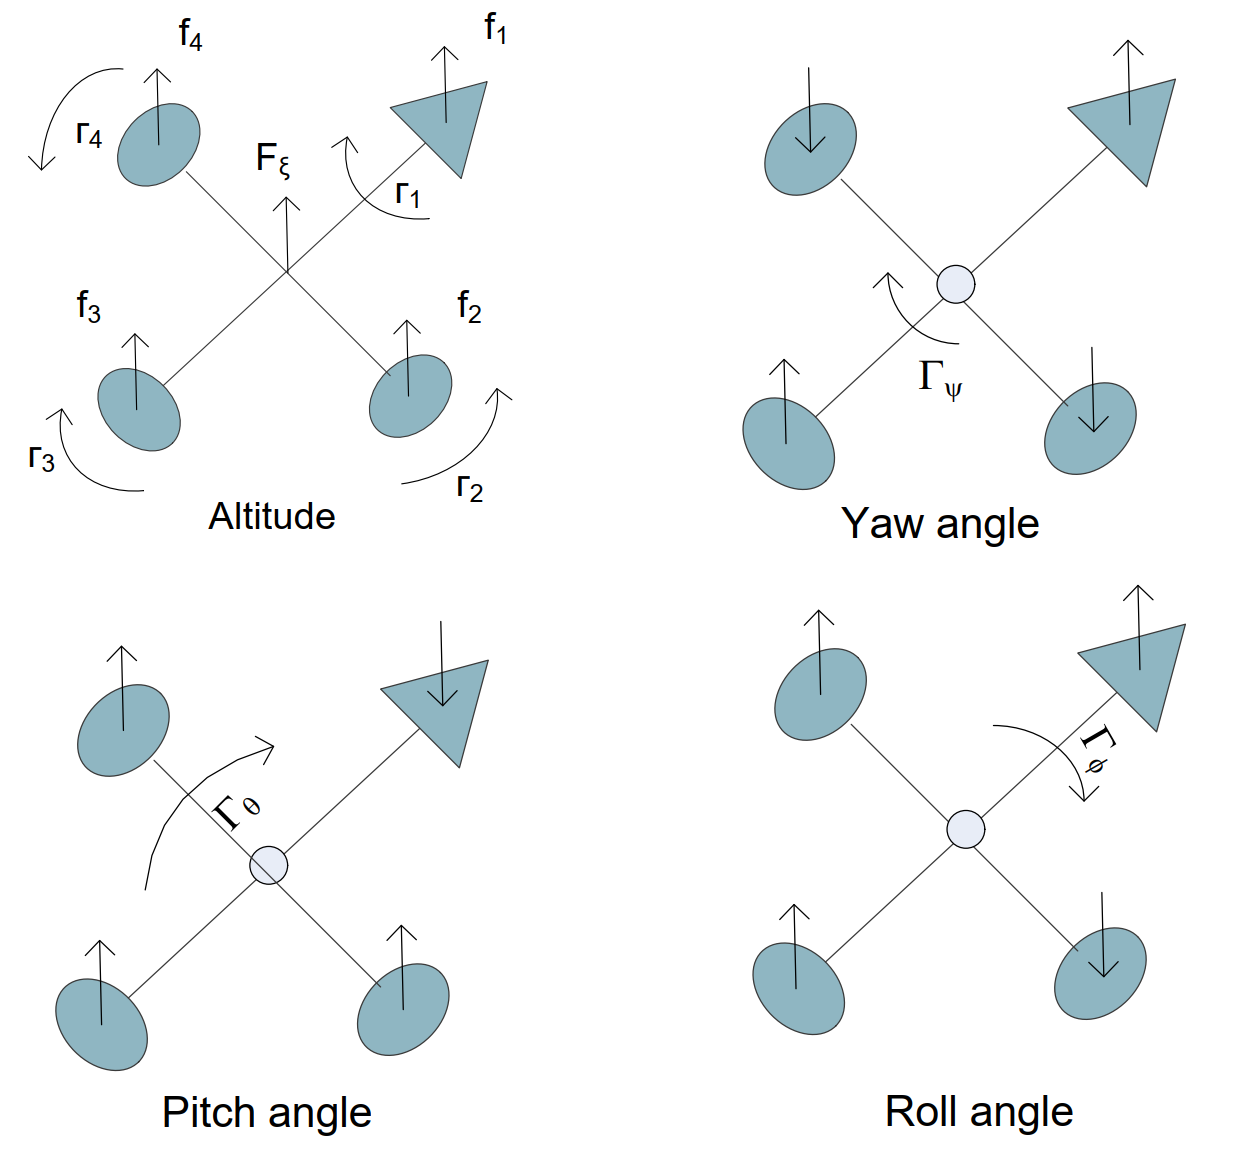
\includegraphics[width=0.6\textwidth]{Images/Modeling/Fantoni_a}
\caption{Model of the quadrotor represented with motor torques and Euler angles \cite{Fantoni2016}.}
\label{Fantoni_a}
\end{figure}

The quadrotor's model \cite{Bouabdalla2007}, when the Euler-Lagrange formalism is used \cite{houston_2001}, is founded on the equations of energy of the mechanical system. The Newton-Euler formalism is given in \cite{Murray1994}. In both cases, the model is computed based on the following assumptions:

\begin{itemize}
	\item The quadrotor has a rigid structure.
	\item The quadrotor has a symmetrical structure.
	\item The center of gravity (CoG) and the fixed frame at the center of the body are assumed to be coincident.
	\item The propellers of the quadrotor are assumed to be rigid.
	\item The thrust and drag forces are assumed to be proportional to the square of the spinning speed of each propeller.
\end{itemize}


\newpage

\subsection{Euler-Lagrange Formalism}

The Lagrangian is expressed as follows:

\begin{equation}
	L(q,\dot{q}) = T_{Trans} + T_{rot} - U = L_{Trans} + L_{Rot}
\end{equation}

with:

\begin{itemize}
	\item $q$: generalized coordinates.
	\item $U$: Potential energy ($U=mgU_z$)
	\item $L_{Rot} = T_{Rot}$ 
\end{itemize}

By utilizing the Euler-Lagrange equations expressed in (\ref{Euler_Lagrange_equations}) below, the equations of motion can be inferred:


\begin{equation}\label{Euler_Lagrange_equations}
	\frac{d}{dt}\bigg(\frac{\partial L(q_i, \dot{q}_i)}{\partial \dot{q}_i} \bigg) -\frac{\partial L (q_i,\dot{q_i})}{\partial q_i} = \tau_i = \begin{bmatrix}
	F_{\xi}\\
	\tau \\
	\end{bmatrix}
\end{equation}

with $F_{\xi}$ depicting the translation forces expressed in the mobile frame and $\tau$ depicting the torques. Thus, the Euler-Lagrange equations can be decomposed into two parts, the part dealing with the translation, and the second part dealing with the rotation. \\
First, the focus will be on the part related to the translation.

\subsection*{Translation Model}

The translational equations on the fixed frame are expressed as follows:

\begin{equation}\label{E_L_Translation}
\frac{d}{dt}\bigg(\frac{\partial L_{Trans}}{\partial \dot{\xi}}\bigg) - \frac{\partial L_{Trans}}{\partial \xi} = F_{\xi}
\end{equation} 

The Lagrangian of translation in the frame $R_O$ is expressed as follows:

\begin{equation}
	L_{Tran}=T_{Trans}-U = \frac{1}{2}m \dot{\xi}^{\intercal} \dot{\xi} - mgz
\end{equation}

With $T_{Trans}=\frac{1}{2}m \dot{\xi}^{\intercal} \dot{\xi}$ representing the kinetic energy which is expressed in the fixed frame such that $\dot{\xi}=\begin{bmatrix}
\dot{x} && \dot{y} && \dot{z} \\
\end{bmatrix}^{\intercal}$ is expressed the fixed frame $R_O$. \\
$F_{\xi}$ must be expressed in $R_{O}$ for the purpose of obtaining the equations of translation in the fixed frame, because $F_{\xi}$ is typically measured in the mobile frame $R_U$.

First, the derivative of $L_{Trans}$ must be calculated with respect to $\dot{\xi}$

\begin{equation}\label{Translational_E_L_a}
	\frac{\partial L_{Trans}}{\dot{\xi}} = \frac{\partial (\frac{1}{2} m \dot{\xi}^{\intercal} \dot{\xi})}{\partial \dot{\xi}}= m \dot{\xi}
\end{equation}

After that, equation (\ref{Translational_E_L_a}) can be differentiated with respect to time as follows: 

\begin{equation}
	\frac{d}{dt}\bigg( \frac{\partial L_{Trans}}{\dot{\xi}} \bigg) = \frac{d}{dt}(m \dot{\xi}) = m \ddot{\xi}
\end{equation} 

Then, $L_{Trans}$ is now differentiated with respect to $\xi$ as follows:

\begin{equation}
	\frac{\partial L_{Trans}}{\partial \xi}=mg\overrightarrow{U_z}
\end{equation}

\newpage

Thus, the final model of the translation in the mobile frame becomes:

\begin{equation}
	\frac{d}{dt}\bigg( \frac{\partial L_{Trans}}{\partial \dot{\xi}} \bigg) - \frac{\partial L_{Trans}}{\partial \xi} = F_{\xi} \Rightarrow m\ddot{\xi} + mg \overrightarrow{U_z} = F_{\xi}
\end{equation}

Finally, all that is left is to transform the forces of translation and express them in the fixed frame in order to obtain the equations of translation in the fixed frame:

\begin{multline}
F_{\xi}= \prescript{O}{}{\begin{bmatrix}
0\\
0\\
-mg
\end{bmatrix}} + \prescript{U}{}{\begin{bmatrix}
0 \\
0 \\
u \\
\end{bmatrix}} \Rightarrow {}^{O}F_{\xi} = \prescript{O}{}{\begin{bmatrix}
0\\
0\\
-mg
\end{bmatrix}} + \prescript{O}{}{\begin{bmatrix}
0 \\
0 \\
u \\
\end{bmatrix}}\\
\Rightarrow {}^{O}F_{\xi} =  \prescript{O}{}{\begin{bmatrix}
0 \\
0 \\
-mg \\
\end{bmatrix}} + {}^{O}A_U  \prescript{O}{}{\begin{bmatrix}
0 \\
0 \\
u \\
\end{bmatrix}} = \prescript{O}{}{\begin{bmatrix}
(\sin \psi \sin \phi + \cos \psi \sin \theta \cos \phi)u \\
(- \sin \phi \cos \psi + \sin \psi \sin \theta \cos \phi )u \\
\cos \theta \cos \phi u -mg \\
\end{bmatrix}}
\end{multline}

Thus, the translational model of the quadrotor can finally be expressed as follows:


\begin{equation}\label{translational_model_E_L}
\begin{cases}
m \ddot{x} = (\sin \psi \sin \phi + \cos \psi \sin \theta \cos \phi)u \\
m \ddot{y} = (- \sin \phi \cos \psi + \sin \psi \sin \theta \cos \phi )u \\
m \ddot{z} = \cos \theta \cos \phi u -mg \\
\end{cases}
\end{equation}

The translation model in (\ref{translational_model_E_L}) can be simplified if small angles of order 2 for pitch and roll are used:



\begin{equation}\label{translational_model_E_L_Simplified}
\begin{cases}
m \ddot{x} = (\phi \sin \psi + \theta \cos \psi)u \\
m \ddot{y} = (- \phi \cos \psi + \theta \sin \psi)u \\
m \ddot{z} = u - mg \\
\end{cases}
\end{equation}

Thus, it can be observed that in this case, the vertical dynamics is fully decoupled from the rest of the system.

Now, as for the physical interpretation of this case:


\begin{figure}[h]
\centering
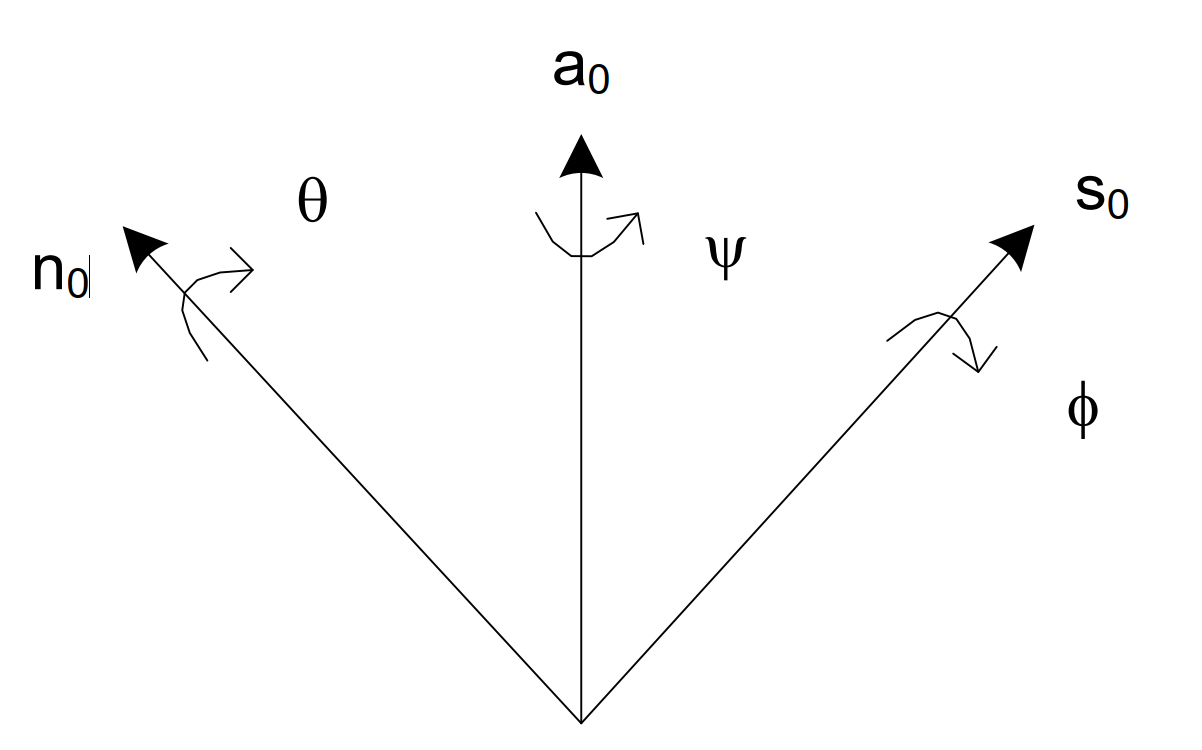
\includegraphics[width=0.5\textwidth]{Images/Modeling/Fantoni_b}
\caption{Angles of rotation \cite{Fantoni2016}.}
\label{Fantoni_b}
\end{figure}

\newpage

If small angles are considered for the following types:

\begin{itemize}
	\item Case 1: $\theta$ small, $\phi=0$
	
	
\begin{figure}[h]
\centering
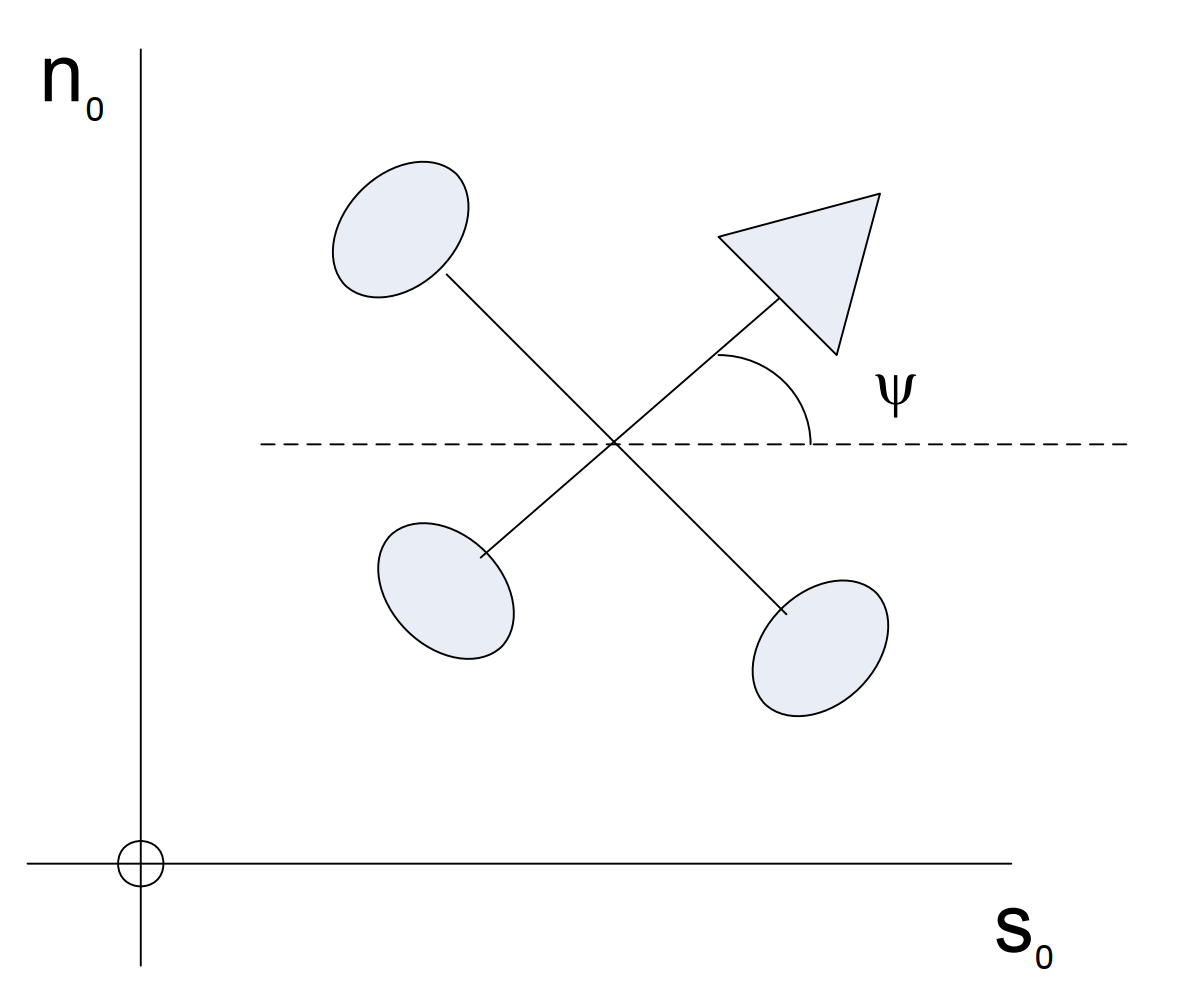
\includegraphics[width=0.5\textwidth]{Images/Modeling/Fantoni_c}
\caption{Top view of the quadrotor \cite{Fantoni2016}.}
\label{Fantoni_c}
\end{figure}	
	
	\begin{equation}\label{E_L_simplified_case_1}
	\begin{cases}
	m \ddot{x} = \theta \cos \psi u \\
	m \ddot{y} = \theta \sin \psi u \\
	m \ddot{z} = u - mg 
	\end{cases}
	\end{equation}
	
	As can be observed from equation (\ref{E_L_simplified_case_1}), the pitch angle $\theta$ is not zero. This means that the quadrotor is tilted forward. Thus, equation(\ref{E_L_simplified_case_1}) shows that the more the UAV is tilted, the more it accelerates. And, if for example $\psi=\frac{\pi}{2}$, it means that $m \ddot{x}=0$ and $m\ddot{y}=\theta u$, so the quadrotor will progress forward along the axis of $n_0$ (figure \ref{Fantoni_c}).  And if $\psi = 0$, it means that $m\ddot{x}= \theta u$ and $m\ddot{y}=0$, so the quadrotor will progress forward along the axis of $s_o$ (figure \ref{Fantoni_c}).
	
	\item Case 2: $\theta=0$, $\phi$ is small
	\begin{equation}\label{E_L_simplified_case_3}
	\begin{cases}
	m \ddot{x} = \phi \sin \psi u \\
	m \ddot{y} = -\phi \cos \psi u \\
	m \ddot{z} = u - mg 
	\end{cases}
	\end{equation}	
	
	In this case, the quadrotor is tiled on the left or right side. If, for instance, $\psi=0$:
	
	\begin{itemize}
		\item $m\ddot{x}=0$ which is natural because in this case, the quadrotor can only roll.
		\item $m\ddot{y}=-\phi u$. So, if the quadrotor has to move forward along the $n_0$ axis (figure \ref{Fantoni_c}), the $\phi$ must be negative.
	\end{itemize}
\end{itemize}

Now, moving on to the rotational model.

\subsection*{Rotational Model}

Contrarily to translational model, the rotational model in the fixed frame is tedious to compute. It is usually computed in the mobile frame for computational simplicity. Indeed, $L_{rot} $ includes the expression of the inertia, which is constant with respect to the mobile frame. Whereas in the fixed frame, the expression of inertia will not be constant anymore, and when $L_{rot}$ is differentiated with respect to time, the complexity of the calculation will increase \cite{Etkin1996}. Furthermore, gyroscopic effects are not neglected.

\subsubsection*{Angular Velocities}

A relationship exists between the body-fixed angular velocity vector $\begin{bmatrix}
p && q && r \\
\end{bmatrix}^{\intercal}$, and the rate of change of the Euler angles $\begin{bmatrix}
\dot{\phi} && \dot{\theta} && \dot{\psi}
\end{bmatrix}^{\intercal}$. This relationship can be found by resolving the Euler rates into the body-fixed coordinate frame.

Based on the theorem of decomposition of rotations, which is expressed as follows:

\begin{equation*}
\overrightarrow{\Omega} = \Omega_x \overrightarrow{x} + \Omega_y \overrightarrow{y} + \Omega_z \overrightarrow{z} + 
\end{equation*}

In the equation above, the three vectors express the rotation vectors and the vector $\overrightarrow{\Omega}$ is the vector of rotation in general. Moreover, the angular velocity of the body-fixed frame usually called $\eta = \begin{bmatrix}
p \\  
q \\
r \\
\end{bmatrix}$

The expression of $\eta$ can be expressed in terms of the variations of Euler angles:

\begin{equation*}
{}^{U}\eta = \dot{\psi} \overrightarrow{a_0} + \dot{\theta} \overrightarrow{n_1} + \dot{\psi} \overrightarrow{s_2}
\end{equation*}

where $\overrightarrow{n_1}$ represents the intermediate axis of rotation which is observed in figure \ref{Fantoni_d}.

\begin{equation*}
	{}^{U}\overrightarrow{\eta} = Rot(-\phi)Rot(-\theta)\begin{bmatrix}
	0 \\
	0 \\
	\dot{\psi}
	\end{bmatrix} + Rot(-\phi) \begin{bmatrix}
	0 \\
	\dot{\psi} \\
	0 
	\end{bmatrix} + \begin{bmatrix}
	\dot{\phi}\\
	0\\
	0
	\end{bmatrix}
\end{equation*}

\begin{equation}\label{eta_Euler_angles_equation}
	{}^{U}\overrightarrow{\eta} = \begin{bmatrix}
	1 && 0 && -\sin \theta \\
	0 && \cos \phi && \cos \theta \sin \phi \\
	0 && - \sin \phi && \cos \phi \cos \theta 
	\end{bmatrix}
	\begin{bmatrix}
	\dot{\phi}\\
	\dot{\theta}\\
	\dot{\psi}
	\end{bmatrix}
\end{equation}

Then, the transition matrix $R_r$ which expresses the decomposition of the angular velocity vector $\overrightarrow{\eta}$ with respect to $\begin{bmatrix}
\dot{\phi} && \dot{\theta} && \dot{\psi}
\end{bmatrix}^{\intercal}$ in the mobile frame \cite{Etkin1996} and \cite{Goldstein1980} is defined as follows:


\begin{equation}
R_r = \begin{bmatrix}
1 && 0 && -\sin \theta \\
0 && \cos \phi && \cos \theta \sin \phi \\
0 && -\sin \phi && \cos \phi \cos \theta \\
\end{bmatrix}
\end{equation}


So, the angular velocity vector expressed in the mobile frame is: 

\begin{equation}
{}^{U}\overrightarrow{\eta}= R_r \begin{bmatrix}
\dot{\phi} \\
\dot{\theta} \\
\dot{\psi} \\
\end{bmatrix}
\end{equation}

Thus, by expanding equation (\ref{eta_Euler_angles_equation}), the following is obtained:

\begin{equation}\label{p_q_r}
	\begin{cases}
		p = \dot{\phi} - \dot{\psi} \sin \theta \\
		q = \dot{\theta} \cos \phi + \dot{\psi} \cos{\theta} \sin{\phi}\\
		r = -\dot{\theta}\sin{\phi} + \dot{\psi} \cos{\phi} \cos{\theta}
	\end{cases}
\end{equation}


\newpage

\subsection{Newton-Euler Formalism}\label{N_E_section}

\subsection*{Translational Model}

Based on the Newton's second law:

\begin{equation}
	\sum \overrightarrow{F}=m\overrightarrow{a}
\end{equation}

with



\begin{itemize}
	\item $\overrightarrow{F}=\overrightarrow{F}_{\xi}=\begin{bmatrix}
F_x \\
F_y \\
F_z \\
\end{bmatrix}$ : vector of external forces.

\item $\overrightarrow{a} = \begin{bmatrix}
\ddot{x} \\
\ddot{y} \\
\ddot{z} \\
\end{bmatrix}$: accelerations vector.
\item $m$: mass of the quadrotor.
\end{itemize}

So, by applying Newton's second law on the quadrotor problem at hand:

\begin{equation*}
	m\begin{bmatrix}
	\ddot{x}\\
	\ddot{y}\\
	\ddot{z}\\
	\end{bmatrix} = \prescript{O}{}{\begin{bmatrix}
	0 \\
	0 \\
	-mg 
	\end{bmatrix}} + \prescript{U}{}{\begin{bmatrix}
	0 \\
	0 \\
	u 
	\end{bmatrix}} = \prescript{O}{}{\begin{bmatrix}
	0 \\
	0 \\
	-mg 
	\end{bmatrix}} + b \prescript{U}{}{\begin{bmatrix}
	0 \\
	0 \\
	\omega_1^2 + \omega_2^2 + \omega_3^2 + \omega_4^2
	\end{bmatrix}}
\end{equation*}


If $u$ is then expressed in the fixed frame, the equations of the translational model  in (\ref{translational_model_E_L}) that were found using the Euler-Lagrange formalism, are found again here:

\begin{equation}\label{translation_model_N_E}
\begin{cases}
m \ddot{x} = (\sin \psi \sin \phi + \cos \psi \sin \theta \cos \phi)u \\
m \ddot{y} = (- \sin \phi \cos \psi + \sin \psi \sin \theta \cos \phi )u \\
m \ddot{z} = \cos \theta \cos \phi u -mg \\
\end{cases}
\end{equation}



\subsection*{Rotational Model}

Based on the Newton-Euler equations, for a rotating frame \cite{Murray1994}: 

\begin{equation}\label{rotational_model_N_E_general_formula}
I \dot{\omega} + \omega \times I \omega = \tau
\end{equation}
with

\begin{itemize}
	\item $I = \begin{bmatrix}
	I_{xx} && 0 && 0 \\
	0 && I_{yy} && 0 \\
	0 && 0 && I_{zz} \\
	\end{bmatrix}$
	\item $\eta=\begin{bmatrix}
	p \\
	q \\
	r \\
	\end{bmatrix}$
	\item $\tau = \begin{bmatrix}
	\tau_1 \\
	\tau_2 \\
	\tau_3 \\
	\end{bmatrix}$
\end{itemize}

Thus, equation (\ref{rotational_model_N_E_general_formula}) becomes:

\begin{equation}
\begin{bmatrix}
I_{xx}\dot{p}\\
I_{yy}\dot{q}\\
I_{zz}\dot{r}\\
\end{bmatrix}+ \begin{bmatrix}
qr(I_{zz}-I_{yy})\\
pr(I_{xx}-I_{zz})\\
pq(I_{yy}-I_{xx})
\end{bmatrix} = \begin{bmatrix}
\tau_1 \\
\tau_2 \\
\tau_3
\end{bmatrix}
\end{equation}


If equation \ref{total_torque_equation} is used, then input vector $\tau$ can be substituted to acquire the final model of the rotation in the body frame:

\begin{equation}
\begin{cases}
\dot{p} = qr \frac{(I_{yy}-I_{zz})}{I_{xx}} + \frac{l}{I_{xx}}(f_4-f_2) - \frac{1}{I_{xx}}qJ_r (\omega_1 - \omega_2 + \omega_3 - \omega_4) \\
\dot{q} = pr \frac{(I_{zz}-I_{xx})}{I_{yy}} + \frac{l}{I_{yy}}(f_3-f_1) + \frac{1}{I_{yy}}pJ_r (\omega_1 - \omega_2 + \omega_3 - \omega_4) \\
\dot{r} = pq \frac{(I_{xx}-I_{yy})}{I_{zz}} + \frac{1}{I_{zz}} d (\omega_1^2 -\omega_2^2 + \omega_3^2 - \omega_4^2)
\end{cases}
\end{equation}

If the nonlinear model is then simplified by using very small angles, then $\begin{bmatrix}
p \\ 
q \\
r \\ 
\end{bmatrix} \approx \begin{bmatrix}
\dot{\phi} \\
\dot{\theta} \\
\dot{\psi} \\
\end{bmatrix}$ will be obtained from equation (\ref{p_q_r}), and the following model of rotation is obtained:

\begin{equation}\label{N_E_rotation_equation_small_angles}
\begin{cases}
\ddot{\phi} = \dot{\theta} \dot{\psi} \frac{(I_{yy}-I_{zz})}{I_{xx}} + \frac{l}{I_{xx}}(f_4-f_2) - \frac{1}{I_{xx}} \dot{\theta} J_r (\omega_1 - \omega_2 + \omega_3 - \omega_4) \\
\ddot{\theta} = \dot{\psi} \dot{\phi} \frac{(I_{zz}-I_{xx})}{I_{yy}} + \frac{l}{I_{yy}}(f_3-f_1) + \frac{1}{I_{yy}} \dot{\phi} J_r (\omega_1 - \omega_2 + \omega_3 - \omega_4) \\
\ddot{\psi} = \dot{\theta} \dot{\phi} \frac{(I_{xx}-I_{yy})}{I_{zz}} + \frac{1}{I_{zz}} d (\omega_1^2 -\omega_2^2 + \omega_3^2 - \omega_4^2)
\end{cases}
\end{equation}

It should be noted that equation (\ref{N_E_rotation_equation_small_angles}) is only valid for very small angles.



\newpage

 \section{State-Space Model}
The translational and rotational models (\ref{translation_model_N_E}) and (\ref{N_E_rotation_equation_small_angles}) respectively that were developed in subsection \ref{N_E_section} express the differential equations of the system. However, for the purpose of control design, it is desirable to reduce the complexity and simplify the model to satisfy the real-time limitations of the embedded control loop. Thus, the thrust and the drag coefficients are assumed to be constant. As a result, the system can be expressed in state-space form \\ $\dot{\textbf{\textsc{x}}}=f(\textbf{\textsc{x}},\textbf{\textsc{u}})$ with $\textbf{\textsc{x}}$ the state vector and $\textbf{\textsc{u}}$ the control input vector.

The state vector has the following form:

\begin{equation}\label{state_vector}
\textbf{\textsc{x}} = \left[\begin{array}{c c c c c c c c c c c c c}
\phi & \dot{\phi} & \theta & \dot{\theta} & \psi & \dot{\psi} & z & \dot{z} & x & \dot{x} & y & \dot{y} 
\end{array}\right]^{\intercal}
\end{equation}
  
 With,
 
\begin{multicols}{2}
 
\begin{equation*}
\begin{aligned}
x_1 = \phi\\
x_2 = \dot{x}_1=\dot{\phi}\\
x_3 = \theta\\
x_4 = \dot{x}_3 = \dot{\theta} \\
x_5 = \psi \\
x_6 = \dot{x}_5 = \dot{\psi}\\
\end{aligned}
\end{equation*}

\columnbreak

\begin{equation}
\begin{aligned}
x_7 = z\\
x_8 = \dot{x}_7=\dot{z}\\
x_9 = x\\
x_{10} = \dot{x}_9 = \dot{x} \\
x_{11} = y \\
x_{12} = \dot{x}_{11} = \dot{y}\\
\end{aligned}
\end{equation}

\end{multicols}
 
Moreover, the control input vector has the following form: 

\begin{equation}\label{control_input_vector}
\textbf{\textsc{u}} = \left[\begin{array}{c c c c}
u_1 & u_2 & u_3 & u_4 
\end{array}\right]^{\intercal}
\end{equation}

Where the control inputs are mapped by: 

\begin{equation}\label{Control_input_mapping}
\begin{cases}
u_1 = b(\omega_1^2 + \omega_2^2 + \omega_3^2 + \omega_4^2)\\
\\
u_2 = b(-\omega_2^2 + \omega_4^2)\\
\\
u_3 = b(\omega_1^2 - \omega^3)\\
\\
u_4 = d(-\omega_1^2 + \omega_2^2 - \omega_3^2 + \omega_4^2) \\
\end{cases}
\end{equation}

As stated earlier when defining equation (\ref{N_E_rotation_equation_small_angles}), the  transformation matrix between the rate of change of the attitude angles ($\dot{\phi},\dot{\theta},\dot{\psi}$) and the angular velocities of the body $(p,q,r)$ can be regarded as the identity matrix if the disturbances due to hover flight are small. As a result, the following can be written:

\begin{equation}
(\dot{\phi},\dot{\theta},\dot{\psi})  \approx (p,q,r)
\end{equation}

Simulation tests have demonstrated that this assumption is reasonable \cite{Bouabdalla2007}. 

\newpage

From equations (\ref{translation_model_N_E}), (\ref{N_E_rotation_equation_small_angles}),(\ref{state_vector}) and (\ref{control_input_vector}), the following expression is obtained after simplification:

\begin{equation}\label{state_space_model}
f(\textbf{\textsc{x}},\textbf{\textsc{u}}) = \begin{pmatrix}
\dot{\phi}\\
\dot{\theta} \dot{\psi} a_1 + \dot{\theta} a_2 \Omega_r + b_1 u_2 \\
\dot{\theta}\\
\dot{\phi} \dot{\psi} a_3 - \dot{\phi} a_4 \Omega_r + b_2 u_3 \\
\dot{\psi}\\
\dot{\theta} \dot{\psi} a_5 + b_3 u_4 \\
\dot{z}\\
g - (\cos \phi \cos \theta) \frac{1}{m} u_1 \\
\dot{x} \\
u_x \frac{1}{m} u_1\\
\dot{y}\\
u_y \frac{1}{m}u_1\\
\end{pmatrix}
\end{equation}

With, 

\begin{multicols}{2}
 
\begin{equation*}
\begin{aligned}
a_1 &= (I_{yy} - I_{zz})/I_{xx}\\
a_2 &= J_r/I_{xx}\\
a_3 &= (I_{zz} - I_{xx})/I_{yy}\\
a_4 &= J_r/I_{yy}\\
a_5 &= (I_{xx} - I_{yy})/I_{zz}\\
\end{aligned}
\end{equation*}

\columnbreak

\begin{equation}
\begin{aligned}
b_1 &= l/I_{xx}\\
b_2 &=l/I_{yy}\\
b_3 &= l/I_{zz}\\
\end{aligned}
\end{equation}

\end{multicols}

\begin{equation}
	\begin{aligned}
	u_x = (\cos \phi \sin \theta \cos \psi + \sin \phi \sin \psi)\\
	u_y = (\cos \phi \sin \theta \sin \psi - \sin \phi \cos \psi)\\
	\end{aligned}
\end{equation}

It is important to note that the angles and the derivatives of the angles do not depend on the components of the translation in the system represented by equation (\ref{state_space_model}). Contrarily, the translation components depend on the angles. So, the system represented by equation(\ref{state_space_model}) can be depicted as two subsystems, the angle subsystem and the translation subsystem as shown in figure 

\begin{figure}[h]
\centering 
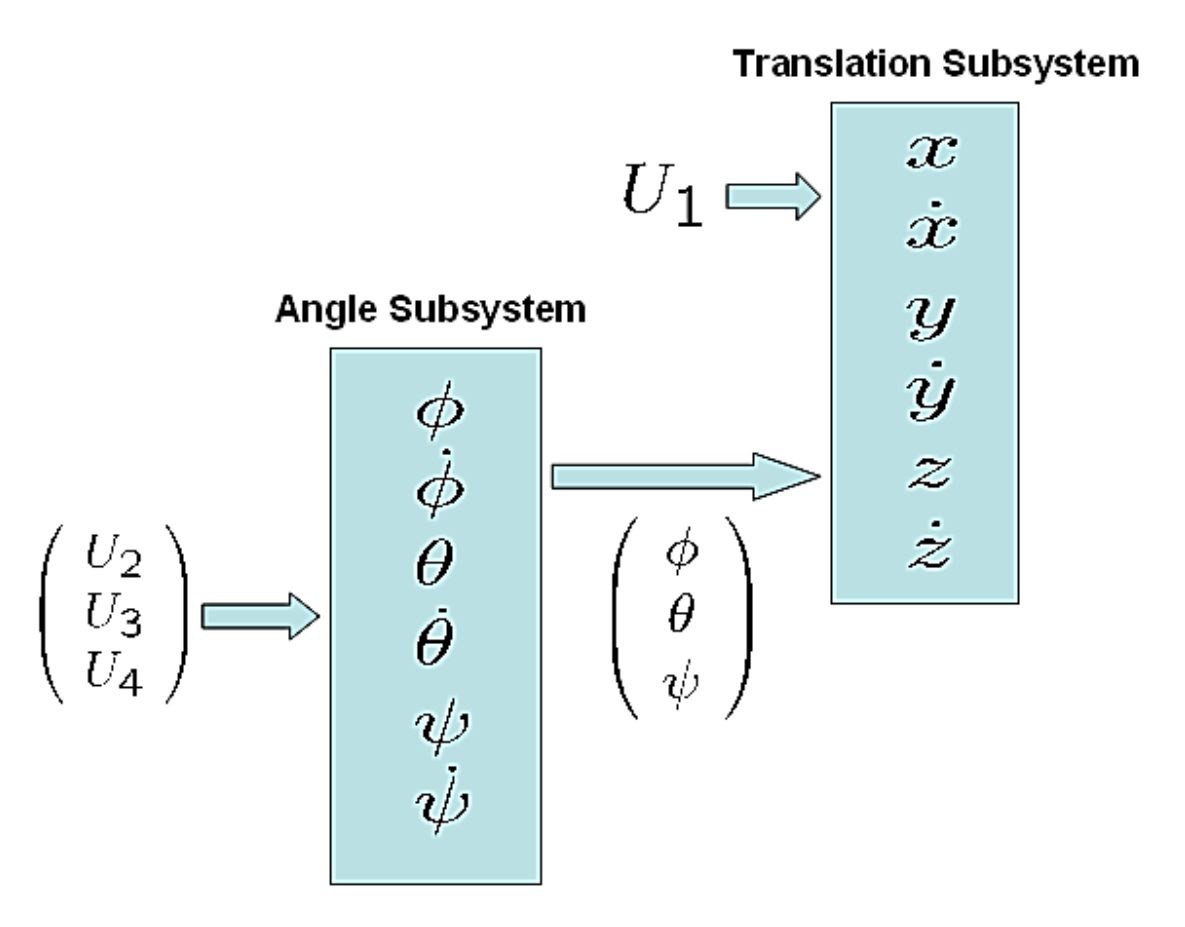
\includegraphics[width=0.5\textwidth]{Images/Modeling/subsystems}
\caption{Link between the rotation and the translation subsystems.\cite{Bouabdalla2007}}
\end{figure}

 \chapter{Control of quadrotors}
In the following sections of this chapter, differential flatness,  the general control architecture of a quadrotor and different potential control approaches (linear and nonlinear) that can be used to control a quadrotor are explained. 
 \section{Differential Flatness}\label{Differential_flatness}  
 
 In the quadrotor community, a well-established finding is that the dynamic model of a quadrotor is differentially flat. Moreover, the control design problem in nonlinear systems will be considerably simplified. Precisely, a system with state $\textbf{\textsc{x}} \in \mathbb{R}^n$ and input $\textbf{\textsc{u}} \in \mathbb{R}^m$ is considered to be \textit{differentially flat} if there exists a set of \textit{flat outputs} $\textbf{\textsc{y}} \in \mathbb{R}^m$ which have the following form:
 
 \begin{equation}
 \textbf{\textsc{y}} = \textbf{\textsc{y}}(\textbf{\textsc{x}}, \textbf{\textsc{u}}, \dot{\textbf{\textsc{u}}},...,\textbf{\textsc{u}}^{(p)})
 \end{equation}

 With, 
 
 \begin{equation}
 	\begin{cases}
 		\textbf{\textsc{x}} = \textbf{\textsc{x}}(\textbf{\textsc{y}}, \dot{\textbf{\textsc{y}}},...,\textbf{\textsc{y}}^{(q)}) \\
 	\\
 		\textbf{\textsc{u}} = \textbf{\textsc{u}}(\textbf{\textsc{y}}, \dot{\textbf{\textsc{y}}},...,\textbf{\textsc{y}}^{(r)}) \\
 	\end{cases}
 \end{equation}

 Thus, the new set of variables is required to be a function of the state, the input and the derivatives of the input. Moreover, this set should also have the same dimensions as the control input. In this manner, it is possible to rewrite both the state and the input in function of the flat outputs and the derivatives of the flat outputs. This is a very useful property in underactuated systems where $m<n$, such as quadrotors, because, it will allow to generate trajectories in the lower dimensional space $m$, then this trajectory will be mapped into the full dimensional \\ space $n$. Another well known example of systems is a car, in which the underactuation is the result of the nonholonomic constraints that are imposed by the wheels. So, for a car, a generated trajectory for $(x,y)$ position of the rear-wheels is enough to specify all the viable trajectories of the system. Formal proofs that the quadrotor system is differentially flat can be found in \cite{Mellinger2011}, and \cite{Faessler2018} for the full model with first-order aerodynamics. The standard choice of flat outputs for the quadrotor is the coodinates of the center of mass and the yaw angle:

\begin{equation}\label{flat_outputs}
\textbf{\textsc{y}} = \begin{bmatrix}
x && y && z && \psi \\
\end{bmatrix}^{\intercal}
\end{equation}

Consequently, the problem of generating a feasible trajectory for a quadrotor then tracking it can be dimensionally decreased from a 6-dimensional space to a 4-dimensional space. By reason of the tight coupling between the rotational and translational dynamics, then defining a trajectory in function of the flat outputs $\textbf{\textsc{y}}$ is sufficient to properly define the full dynamics $\textbf{\textsc{x}}$.


\newpage 
 
 \section{General Control Architecture}
 In the last few years, many researches have developed interest in control of quadrotors. As a result, various control approaches have been proposed. The most known control architecture \cite{Faessler2018} consists of three nested control loops, as shown in figure \ref{General_control_architecture}, in order to generate the suitable thrust in each actuator to follow the desired signal. This strategy assumes that the attitude dynamics of a quadrotor are much faster than the translational dynamics. Assuming that Euler angles are used to define the attitude and that a navigation module generates the desired trajectory $(\bm{r}_d(t),\psi_d(t))$ as shown in section \ref{Differential_flatness}, then:
 
\begin{itemize}
	\setlength{\itemindent}{-.5in}
	\item [] \textbf{Position controller} has the objective of driving the errors occurring on the translational dynamics to zero.
		And, the outputs of this outer loop are the thrust $f=u_1$, which is sent to the motor controller, and the desired attitude $(\theta_d(t),\phi_d(t))$, which corresponds to the reference signal of the attitude controller.
	\item [] \textbf{Attitude controller} has the goal of driving the errors occuring on the rotational dynamics to zero. This controller generates the inputs 
	$\bm{\tau}=\begin{bmatrix}
	u_2 && u_3 && u_4 \\
	\end{bmatrix}^{\intercal}
	$
	that are then sent to the motor controller.
	\item [] \textbf{Motor controller} This controller receives the control inputs 	$\bm{u}=\begin{bmatrix}
	f && \bm{\tau}
	\end{bmatrix}^{\intercal}
	$ and maps them into the desired spinning velocities $\Omega_i$ for each individual rotor based on equation (\ref{Control_input_mapping}). Moreover, low-level control laws are designed and realized in the firmware of the drone to make the convergence from the actual rotations to these desired values.
\end{itemize}
 

 
 \begin{figure}[h]
 \centering
 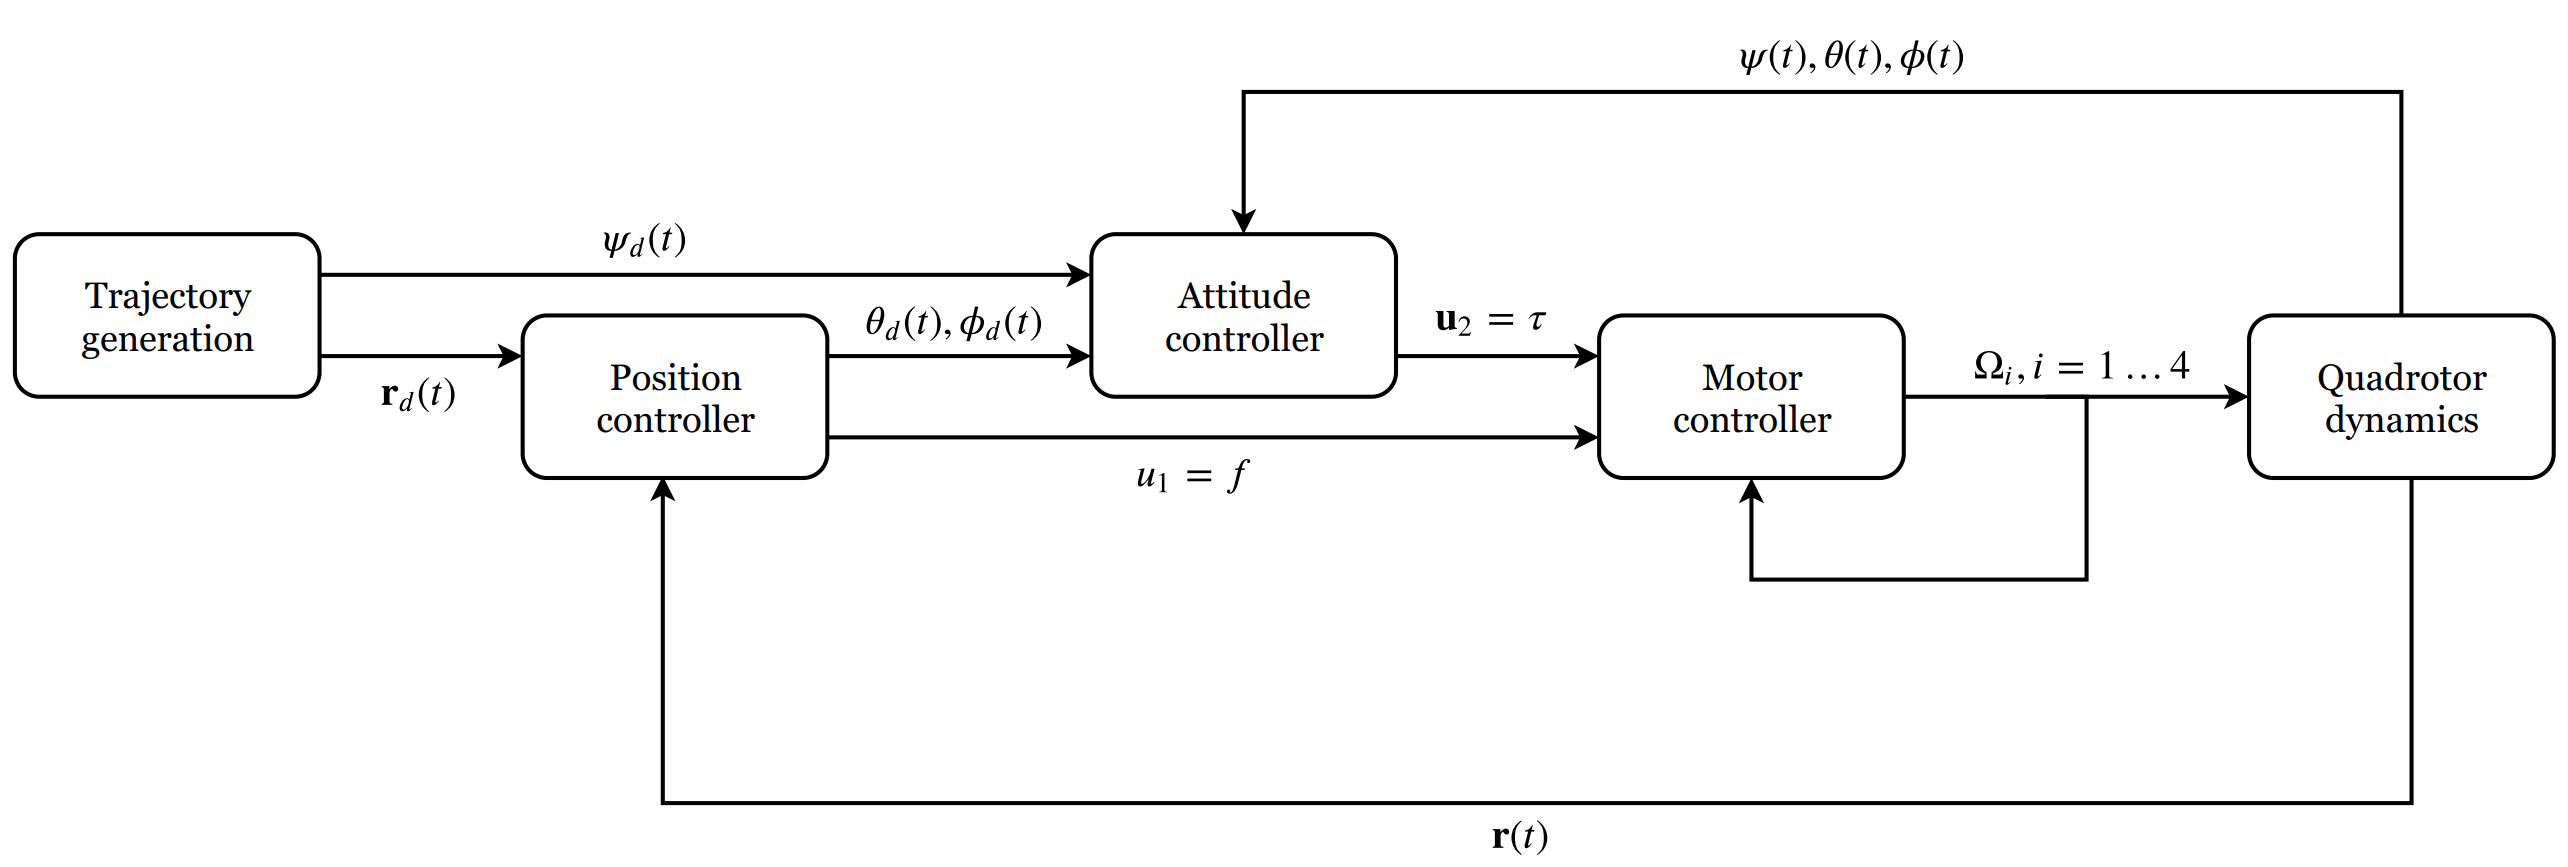
\includegraphics[width=0.8\textwidth]{Images/Control/General_control_architecture}
 \caption{General control architecture of a quadrotor.}
 \label{General_control_architecture}
 \end{figure}
 
 
 
 \newpage 
 \section{General Control Approaches}\label{control_approaches_for_multi_flip_maneuvers}

\subsection{Method of Linearization}

By using extreme assumptions, it is feasible to apply linear control techniques in order to control a quadrotor (\cite{Sabatino2015}, \cite{BouabdallahNothSiegwart2018}). Particularly, this can be made by doing a linearization of the full dynamic model around an equilibrium point $\overline{\textbf{\textsc{x}}}$ and by using the assumption that the vehicle is only capable of oscillating lightly around the hover point.
It is very easy to observe that a feasible equilibrium is provided by a configuration where the center of mass is at a random position $\overline{\textbf{\textsc{r}}}$ and all the other elements of the state are set to zero. So, the nominal input $ \textbf{\textsc{u}} = \overline{\textbf{\textsc{u}}}$ to sustain such equilibrium can be assessed as the thrust that is required to compensate the gravity force:

\begin{equation}
\overline{\textbf{\textsc{u}}} = \begin{bmatrix}
f \\ 
\bm{\tau}\\
\end{bmatrix}=
\begin{bmatrix}
mg \\
\bm{0_{3 \times 1}} \\
\end{bmatrix}
\end{equation}

At this stage, the complete non-linear dynamics that have the form :

\begin{equation}
\dot{\textbf{\textsc{x}}}=\overline{\textbf{\textsc{f}}}(\overline{\textbf{\textsc{x}}},\overline{\textbf{\textsc{u}}})
\end{equation}

can now be linearized around the hover point $(\overline{\textbf{\textsc{x}}},\overline{\textbf{\textsc{u}}})$ as shown below.

\begin{equation}
\dot{\textbf{\textsc{x}}} = \begin{bmatrix}
\frac{\partial \textbf{\textsc{f}}(\textbf{\textsc{x}},\textbf{\textsc{u}})}{\partial \textbf{\textsc{x}}}
\end{bmatrix}_{(\bar{\textbf{\textsc{x}}},\bar{\textbf{\textsc{u}}})} \textbf{\textsc{x}}+ 
\begin{bmatrix}
\frac{\partial \textbf{\textsc{f}}(\textbf{\textsc{x}},\textbf{\textsc{u}})}{\partial \textbf{\textsc{x}}}
\end{bmatrix}_{(\bar{\textbf{\textsc{x}}},\bar{\textbf{\textsc{u}}})} \textbf{\textsc{u}} = \textbf{\textsc{A}}\textbf{\textsc{x}} + \textbf{\textsc{B}} \textbf{\textsc{u}}
\end{equation}

It can be demonstrated that both matrices $\textbf{\textsc{A}}$ and $\textbf{\textsc{B}}$ can be used to determine a linear system that is both controllable and observable \cite{Sabatino2015}. Thus, any control technique that is linear can now be used on the quadrotor in order to keep it around a desired equilibrium point, such as optimal LQR/LQG \cite{Cowling2007,Minh2010} control or simple PD or PID controller \cite{Han2012,Altug2007}.



 \subsection{Internal Lyapunov Stability}
 
Before defining the \textit{Lyapunov Direct Method}, the notions of stability will be thoroughly defined first.

\subsubsection{Notions of Stability}
 For a general system without any control input
 
\begin{align}
 \dot{x}(t) &= f(x(t),0,t) \hspace{1in} (CT) \\
 \dot{x}(k+1) &= f(x(k),0,k) \hspace{1in} (DT),
\end{align}

 it is said that a point $\overline{x}$ is called an \textit{equilibrium point} from time $t_0$ for the continuous system (CT) if $f(\overline{x},0,t)=0,$ $\forall t \geq t_0$. Moreover, in the discrete time (DT) case, the point $\overline{x}$ is an equilibrium point from time $k_0$ if $f(\overline{x},0,k)=0,$ $\forall k \geq k_0$.
If the system begins from state $\overline{x}$ at time $t_0$ or $k_0$, then the system will stay there and will not change with time. It is possible for nonlinear system to have more than one equilibrium point (equilibria). There also exists another class of special solutions in the case of nonlinear systems, these solutions are called \textit{periodic} solution. However, it is outside the scope of this paper and interested readers are referred to \cite{Schmitt1972} for a more in depth explanation. So, the focus will be on equilibria. It is desired to identify the \textit{stability} of the equilibria in some way. For instance, it is desired to know if, given some small perturbation to the system, the state would either come back to the equilibrium point, remain close to it in some sense, or it diverges.

The most useful notion of stability for an equilibrium point of a nonlinear system is provided by the definition below. Assuming that the equilibrium point is at the origin, because if $\overline{x} \neq 0$, a simple translation can be done to obtain a system that is equivalent with the equilibrium at the origin.

\paragraph{Asymptotic stability} A system is said to be \textit{asymptotically stable} about its own equilibrium point at the origin if the following two conditions are satisfied \cite{Dahleh2011}:

\begin{enumerate}
	\item For any $\epsilon > 0$, $\exists \delta_1 > 0$ such that if $\| x(t_0)\|<\delta_1$, then $\|x(t)\|<\epsilon, \forall t>t_0$.
	\item $\exists \delta_2$ such that if $\|x(t_0)\|<\delta_2$, then $x(t)\rightarrow 0$ at $t \rightarrow \infty$.
\end{enumerate}

For the first condition, it is required that the state trajectory should be restricted to a randomly small \textit{"ball"} that is centered at the equilibrium point and has a radius $\epsilon$, when released from an \textit{arbitrary} initial condition in a ball that has an adequately small (yet positive) radius $\delta_1$. This is referred to as \textit{stability in the sense of Lyapunov} (i.s.L.). It is also possible to have stability in the sense of Lyapunov without having asymptotic stability, in that case, it is said that the equilibrium point is \textit{marginally stable}. Moreover, there also exist nonlinear systems that satisfy the second condition without being stable in the sense of Lyapunov. Furthermore, an equilibrium point that is \textit{not} stable in the sense of Lyapunov is said to be \textit{unstable}.

\subsubsection{Lyapunov's Direct Method}

\paragraph{General Idea}

If the following continuous-time system is considered

\begin{equation} \label{Lyapunov_nonlinear_equation}
\dot{x}(t) = f(x(t))
\end{equation}
which has an equilibrium point at the origin (x=0).This system is called a time-invariant system because $f$ does not depend explicitly on the time t. In such a system, the stability analysis of the equilibrium point is in general a tedious task.This is due to the fact that writing a simple formula which relates the trajectory to the initial state is not possible. The main idea of \textit{Lyapunov's direct method} is to determine properties of the equilibrium point (of the nonlinear system in general) by evaluating how a certain carefully chosen scalar function of the changes as the state of the system changes. (The word \textit{"direct"} is utilized to differentiate this method from the Lypunov's \textit{"indirect"} method, which tries to establish properties of the equilibrium point by assessing the behavior of the \textit{linearized} system at that point \cite{MELCHORAGUILAR2004175}.

As an example, a continuous and scalar function $V(x)$ that is equal to 0 at the origin and positive elsewhere is considered in some ball that is enclosing the origin. So, $V(0)=0$ and $V(x)>0$ when $x \neq 0$ in this ball. This $V(x)$ can be considered as an \textit{"energy"} function. Also, let $\dot{V}(x)$ denote the time derivative of $V(x)$ throughout any trajectory of the system. In other words,  $\dot{V}(x)$ varies as $x(t)$ varies proportionally to equation (\ref{Lyapunov_nonlinear_equation}). If this derivative is negative in all the region (with the exclusion of the origin), then this means that the energy is decreasing with time in a strict manner. Moreover, since the lower bound of the energy is 0, then the energy must go to 0 with time. This means that all trajectories will converge to the origin (zero state). This idea is formalized below.




\newpage

\paragraph{Lyapunov Functions}

Assuming V is a continuous map from $\mathbb{R}^n$ to $\mathbb{R}$, $V(x)$ is called a \textit{locally positive definite} (lpd) function about x=0 if 

\begin{enumerate}
	\item $V(0)=0$.
	\item $V(x)>0$, $0<\|x\|<r$ for a given $r$.
\end{enumerate}

Also, the function is called locally \textit{positive semi-definite} (lpsd) if the strict inequality applied on the function in the second condition is changed to $V(x) \geq 0$. The function $V(x)$ is locally \textit{negative definite} (lnd) if $-V(x)$ is lpd. Moreover, $V(x)$ is locally \textit{negative semidefinite} (lnsd) if $-V(x)$ is lpsd. In order to graphically illustrate the locally positive definite function $V(x)$, it is useful to imagine having "contours" of constant $V$ that form (at least in a tiny region about the origin) a set of nested surfaces that are encircling the origin. An example is given in figure \ref{Lyapunov_figure} below. 


\begin{figure}[h]
\centering
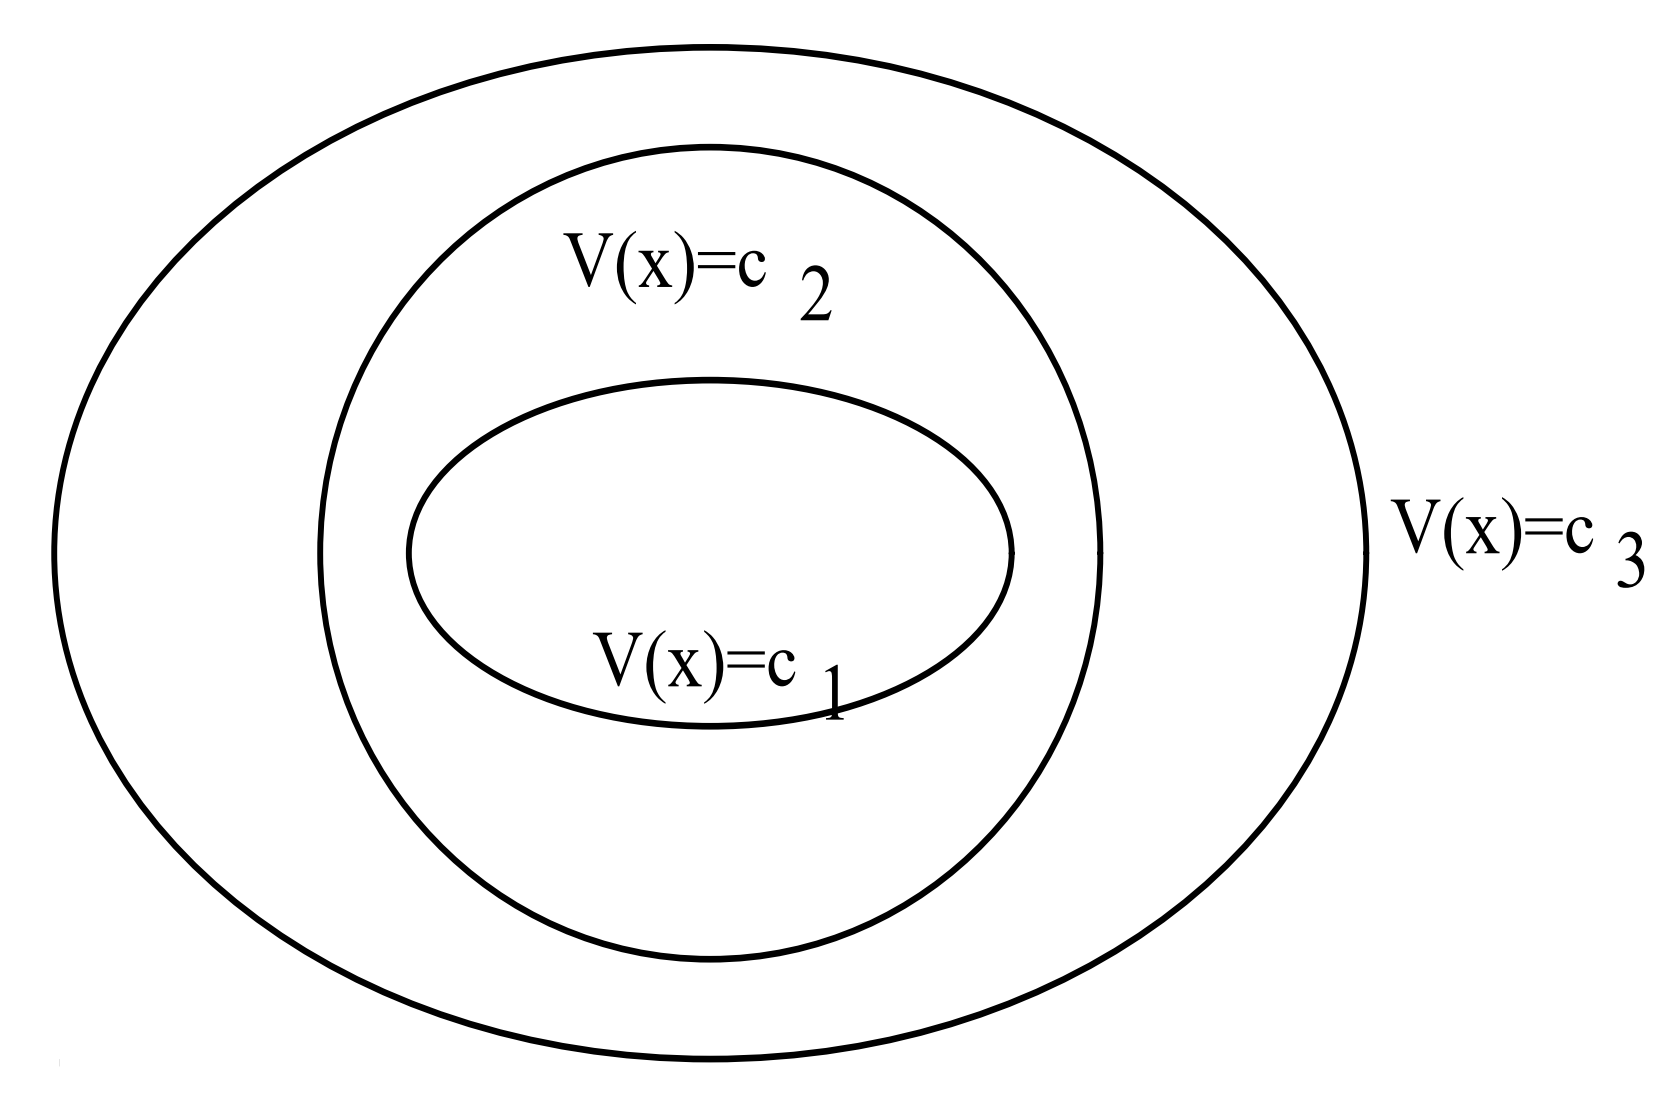
\includegraphics[width=0.6\textwidth]{Images/Control/Lyapunov_function}
\caption{Different values for a Lyapunov function, where $c_1<c_2<c_3$. \cite{Dahleh2011}}
\label{Lyapunov_figure}
\end{figure}

In the continuous time case, the focus in this bibliography will be restricted to $V(x)$ that has first partial derivatives that are continuous. (In the case of discrete time, only continuity will suffice, so differentiability is not required in that case.) The derivative of $V$ with respect to time \textit{along a trajectory of the system} \ref{Lyapunov_nonlinear_equation} is denoted as $\dot{V}(x(t))$. This derivative is expressed as follows:

\begin{equation}
\dot{V}(x(t)) = \frac{dV(x)}{dx}\dot{x} = \frac{dV(x)}{dx}f(x)
\end{equation}
where 
$\frac{dV(x)}{x}$ is the \textit{Jacobian} of $V$ with respect to $x$ which contain the partial derivative $V$ with respect to every component of $x$: $\frac{\partial V}{\partial x_i}$.

Moreover, assuming $V$ is a lpd function (a "candidate Lyapunov function"), and $(\dot{V})$ is the derivative along trajectories of the system of equation \ref{Lyapunov_nonlinear_equation}. Then,$V$ is called a \textit{Lyapunov function} of the system of equation \ref{Lyapunov_nonlinear_equation} if $\dot{V}$ is lnsd \cite{Dahleh2011}.


\paragraph{Lyapunov Theorem for Local Stability}

If a Lyapunov function for the system of equation (\ref{Lyapunov_nonlinear_equation}) exists, this means that $x=0$ is a stable equilibrium point in the sense of Lyapunov. Moreover, if $\dot{V}<0$, $0<\|x\|<r_1$, for some $r_1$, in other words, if $\dot{V}$ is lnd, this means that $x=0$ is an equilibrium point that is asymptotically stable\cite{Dahleh2011}.




\begin{comment}
In order to demonstrate this, the stability in the sense of Lyapunov must first be proven. Assuming that $\epsilon>0$ is given. Then a $\delta>0$ must be found such that for all $\|x(0)\|<\delta$, it follows that $\|x(t)\|<\epsilon$, $\forall t>0$. 

\newpage

The figure \ref{Lyapunov_proof_a} below shows the constructions of the proof.

\begin{figure}[h]
\centering
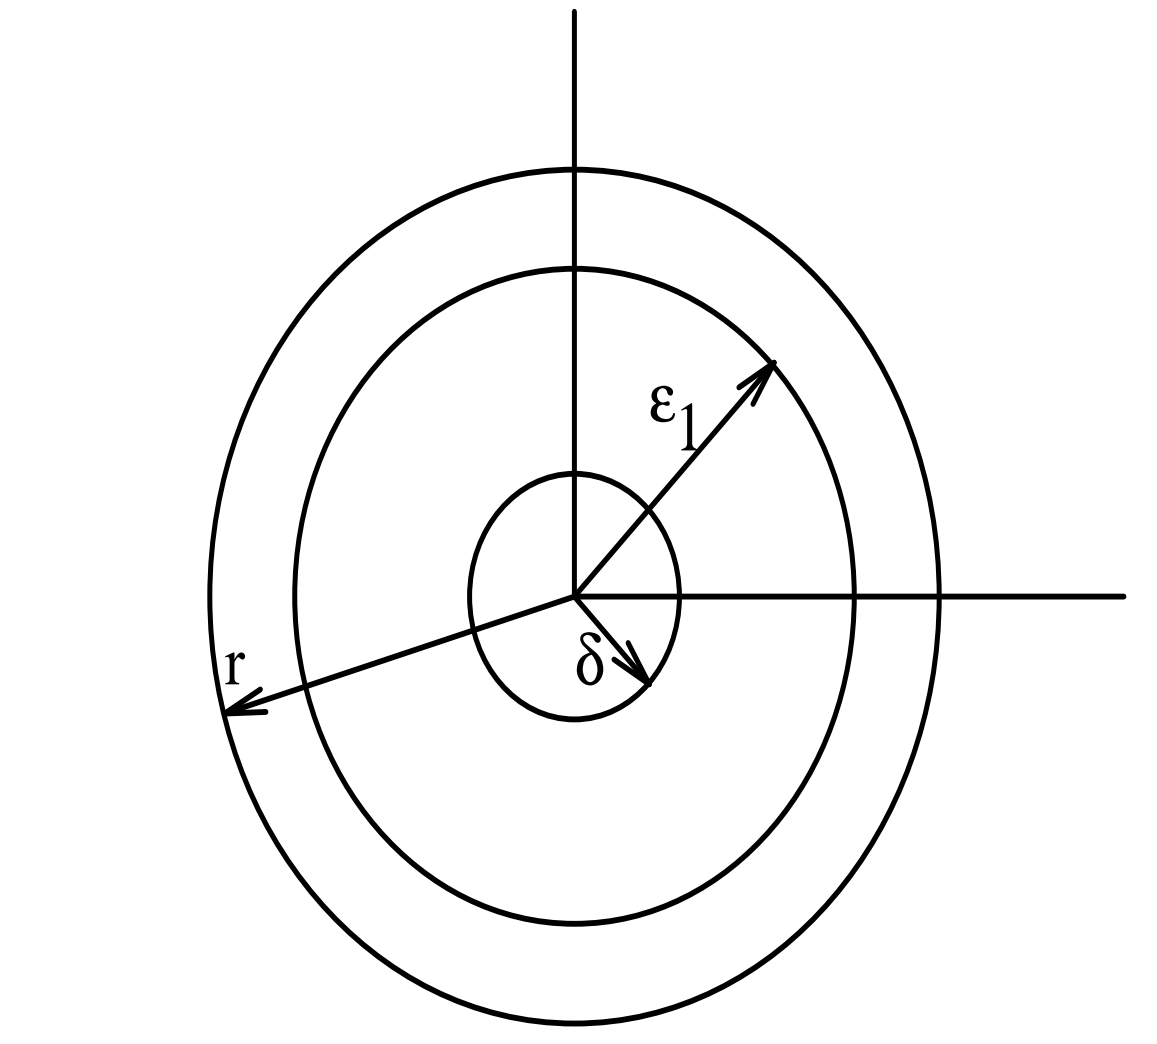
\includegraphics[width=0.6\textwidth]{Images/Control/Proof}
\caption{Representation of the neighborhoods used for the proof \cite{Dahleh2011}.}
\label{Lyapunov_proof_a}
\end{figure}

Let $\epsilon_1 = \min(\epsilon,r)$. And, assuming:

\begin{equation}
m = \min_{\|x\|=\epsilon_1} V(x)
\end{equation}

Since $V(x)$ is continuous, then $m$ is positive and well defined. Then a value $\delta$ can be chosen with $0<\delta<\epsilon_1$ such that for all $\|x\|<\delta$
, $V(x)<m$. 

\end{comment}



\paragraph{Lyapunov Theorem of Global Asymptotic Stability}

The region in the state space for which the earlier results hold is determined by the region over which $V(x)$ represents a Lyapunov function. It is useful to find the \textit{"basin of attraction"} of an equilibrium point that is asymptotically stable. In other words, the basin of attraction is the set of initial conditions whose following trajectories conclude at the equilibrium point. Thus, an equilibrium point is called \textit{"globally asymptotically stable"} ( namely, asymptotically stable "in the large") if its basin of attraction constitutes the full state space of the system.\\

\noindent
If a function $V(x)$ has the following criteria below, 

\begin{enumerate}
	\item $V(x)$ is positive definite throughout the state-space.
	\item $V(x)$ also has the added property that $|V(x)| \rightarrow \infty$ as $\|x\| \rightarrow \infty$.
	\item The derivative of $V$ (in other words $\dot{V}$) is negative definite throughout the state-space.
\end{enumerate}
Then, the equilibrium point at the origin is globally asymptotically stable \cite{Dahleh2011}.

\paragraph{Discrete-Time Systems}

Fundamentally identical results hold for the system

\begin{equation}
x(k+1) = f(x(k))
\end{equation}

provided that $\dot{V}$ is represented as

\begin{equation*}
\dot{V}(x) \triangleq V(f(x)) - V(x),
\end{equation*}

in other words as 

\begin{equation*}
V(\text{next state}) - V(\text{present state})
\end{equation*}


 \subsection{Model Predictive Control}
 \subsubsection{General Idea}\label{MPC_General_Idea}
 
 There exist "open-loop" methods \cite{Kirillova2000} in which the control input sequence $\textbf{\textsc{u}}(t)$ is designed using a model of the system and a set of constraints. However, the problem with this approach is that modeling errors and noise are not taken into consideration. So, these inputs will not necessarily generate the desired response from the system. Because of that, a \textit{"closed-loop"} strategy is required in order to cancel out these errors. So, an approach that can be used is called \textit{"Model Predictive Control"} (MPC). This method is also known as \textit{"receding horizon control"} \cite{How2008} because the \textit{"prediction horizon"} (which is a finite horizon) translates forward by one time step after the current optimization problem is solved . In short, MPC is a \textit{feedback control} algorithm which uses a model of the system to predict the future outputs of the system and it solves an optimization problem on-line in order to select an optimal control.

\newpage 
 
 \paragraph{Basic strategy}

The basic strategy of MPC is following:


\begin{itemize}
	\item At time step $k$, the system model and an optimizer will be used in order to design a sequence of control inputs
	
	$$ \textbf{\textsc{u}}(k|k), \textbf{\textsc{u}}(k+1|k), \textbf{\textsc{u}}(k+2|k), \textbf{\textsc{u}}(k+3|k),...,\textbf{\textsc{u}}(k+N|k) $$
	
	starting from the current state $\textbf{\textsc{x}}(k)$ over a prediction horizon $N$.
	\item Only the first step of the sequence of control inputs will be applied on the system.
	\item The processes above are then iterated for time $(k+1)$ at state $\textbf{\textsc{x}}(k+1)$. 
\end{itemize}
 
 
 \begin{figure}[h]
 \centering
 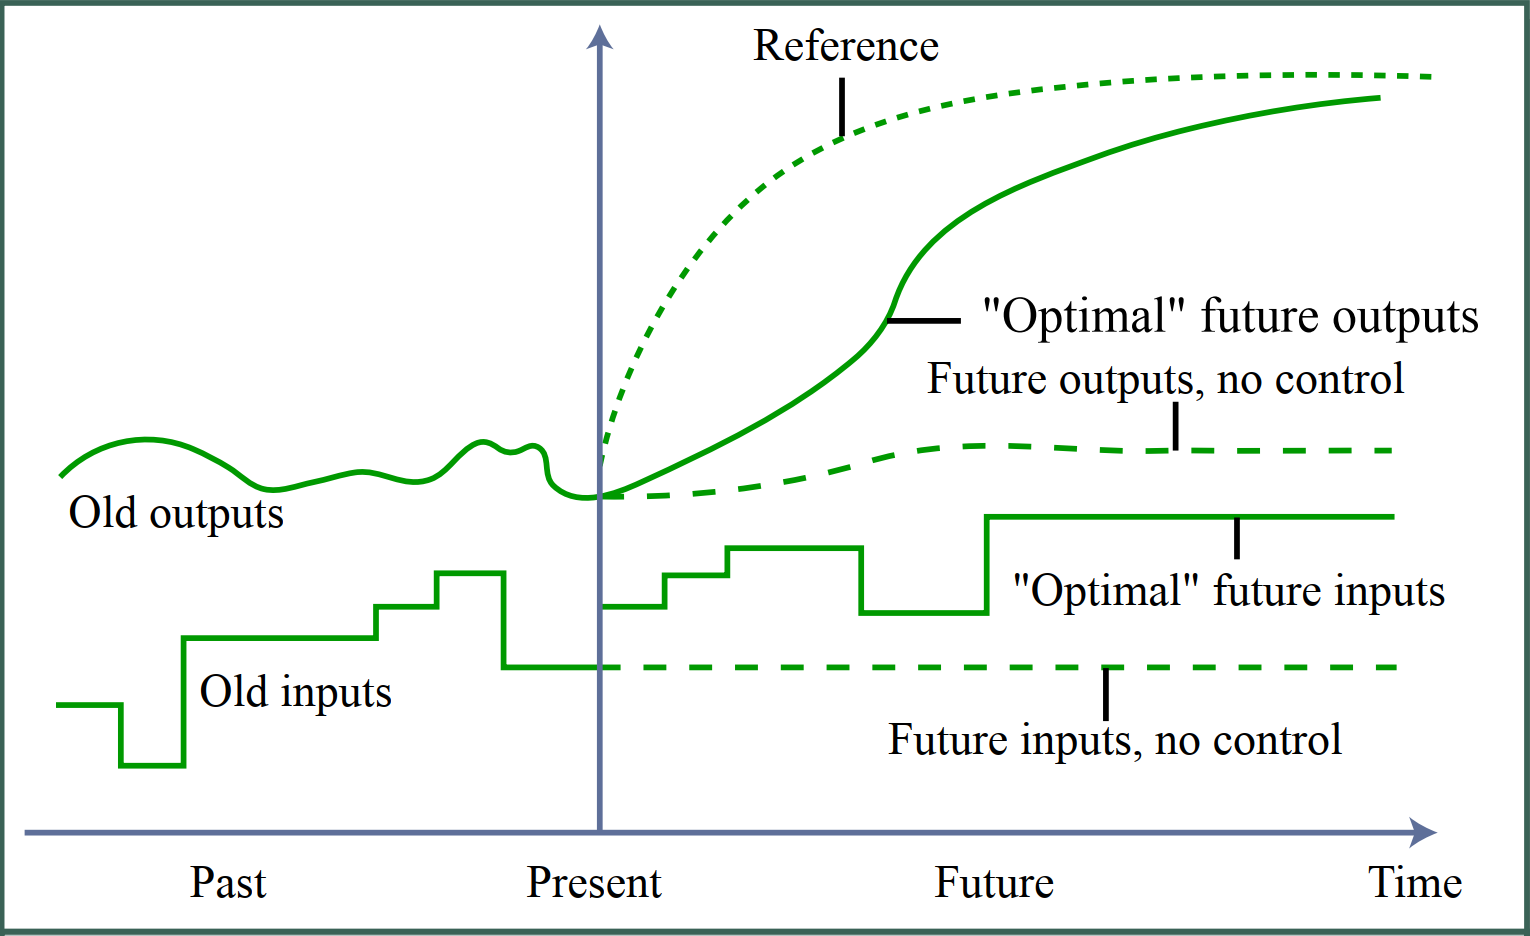
\includegraphics[width=0.6\textwidth]{Images/control/MPC_general_idea}
 \caption{Basic idea of MPC \cite{How2008}.}
 \label{MPC_basic_idea}
\end{figure}  
 
\noindent It should be noted that the control algorithm of MPC is based on numerically solving an optimization problem at each time step. In general, it is a constrained optimization.
 
 \paragraph{Advantages and drawbacks of MPC} There are several advantages when using MPC: 
 
 \begin{itemize}
 	\item MPC is able to control multi-input multi-output (MIMO) systems which might have interactions between their inputs and outputs
 	\item MPC explicitly accounts for the constraints that are imposed on the system. So, it does not just design a controller to keep the system away from the constraints.
 	\item MPC can easily handle nonlinear dynamics and time-varying plant dynamics, because the controller is explicitly a function of the model of the system which can be modified in real-time.
 \end{itemize}

\noindent The main drawback of MPC is that it usually requires a powerful and fast processor with a large memory in order to properly solve the problem at hand, because it solves an optimization problem at each time step.
 
\noindent There have been many commercial applications of MPC starting from the early 1970s in the process industry. The table \ref{table_MPC} below shows the different companies that have used MPC in different industries in 2014.
 
\newpage

\begin{table}[h]
\setlength{\tabcolsep}{15pt} % Default value: 6pt
\renewcommand{\arraystretch}{1} % Default value: 1
 \caption{MPC applications in different industries in 2014 \cite{Kozak2014}.}
 \label{table_MPC}
\begin{tabular}{l c c c c c r}
Application & Aspen & Honeywell & Adersa & CCI & Pavilion & Total \\
\hline
Refining & 950 & 300 & 290 & - & 15 & 1555 \\
Chemicals & 437 & 55 & 12 & 21 & 25 & 550 \\
Food & - & - & 48 & - & 14 & 62 \\
Pulp paper & 21 & 39 & - & - & 3 & 63 \\
Gas and air & 11 & 13 & - & 24 & - & 48 \\
Polymer & 5 & - & - & - & 22 & 27 \\
Utilities & 7 & 9 & - & 6 & - & 22 \\
Other & 39 & - & 51 & 6 & - & 96 \\
\hline 
\hline
Total & 1470 & 416 & 401 & 57 & 79 & 2423 \\
\end{tabular}
\end{table}

\noindent However, as computational power has increased throughout the years thanks to the advancement of technology, there has been a renewed curiosity in applying this control approach to systems with fast dynamics for which the computational complexity is significantly larger when compared to the industrial applications for which computational complexity was not a concern (since MPC was applied on systems with slow dynamics in that case).
 
\subsubsection{Design Parameters}
The different parameters that can be tuned in a MPC controller (\cite{MathWorks2018, MathWorks2018b, MathWorks2018c}) are the following:

\begin{itemize}
	\item The sample time $T_s$.
	\item The prediction horizon $N$.
	\item The control horizon $m$.
	\item The constraints.
	\item The weights.
\end{itemize}

\noindent Choosing the proper values for the parameters stated above is very important since they affect the performance of the controller and the computational complexity of the MPC algorithm.

\paragraph{Sample Time $T_s$} 

The sample time determine the rate at which the controller executes the control algorithm. \begin{itemize}
	\item If $T_s$ is too large, then when a disturbance occurs, the controller will be unable to react to the disturbance quick enough.
	\item If $T_s$ is too small, the controller will have much faster reaction times to disturbances and setpoint changes. However, this comes at the cost of an excessive computational load.
\end{itemize}

\noindent In order to find reasonable balance between controller performance and computational effort, the general recommendation is to have between 10\% and 25\% of the minimum desired close-loop response time .

\paragraph{Prediction horizon $N$} 

The prediction horizon $N$ (sometimes referred to with the variable $p$, however, $N$ will be used instead for the remaining of this paper) is the number of predicted future time steps of the system. It shows how far the controller predicts into the future. Thus, a prediction horizon must be chosen in such a way that it covers the significant dynamics of the system. However, it should be noted that a large prediction horizon should not be selected, since unexpected phenomenons could occur that may affect the dynamics of the system, which will cause a waste of computational power. The general recommendation is to increase $N$ until additional increases will have little impact on the performance. The maximum $N$ is the number of control intervals needed for the open-loop step response of the system to become infinite. However, having $N>50$ is hardly ever required unless $T_s$ is very small.

\paragraph{Control horizon m}

The control horizon is the set of future actions which will lead to the predicted plant output. It represents the number of control moves until time step $m$. After the first $m$ steps, the remaining inputs will remain constant as shown in figure \ref{MPC_basic_idea} for the \textit{"Optimal"} future inputs. Moreover, each control input element in the control horizon is a free variable that will be computed by the optimizer. Thus, the smaller the control horizon, the fewer the computations. However, setting $m=1$ may not give the best possible output for the system. And, similarly to the prediction horizon, if the control horizon is increased, this will lead to better predictions at the cost of increasing the computational complexity. Moreover, the general recommendation for the control horizon is to keep it much smaller than the prediction horizon, because:

\begin{itemize}
	\item A smaller control horizon $m$ will lead to less variables to optimize in the QP that will be solved at each control input interval. This will encourage quicker computation times.
	\item If delays are considered, then having $m<N$ is mandatory. Otherwise, some control input elements within the control horizon  may not have any effect on the plant outputs before the prediction horizon ends, which will lead to a QP Hessian matrix which is singular. 
	\item Having a small value for $m$ encourages having an internally stable controller. However, this is not guaranteed.
\end{itemize}

\paragraph{Constraints} A model predictive controller can integrate constraints on the inputs, the rate of change of the inputs and the outputs. In addition, the constraints can be \textit{"soft"} constraints or \textit{"hard"} constraints. However, it should be noted that hard constraints cannot be violated. In addition, applying hard constraints on both the inputs and outputs at the same time may cause conflict to occur between the constraints, which may lead to an unfeasible solution. Moreover, the general recommendation is to use soft constraints on the outputs and to avoid having hard constraints on both the inputs together with the rate of change of the inputs .

\paragraph{Weights} Model Predictive Control could have many goals. A could could possible be to have the outputs converge to their set-points as fast as possible. Another goal can be to have smooth control inputs in order to avoid aggressive control maneuvers. So, in order to achieve a balanced performance between these two competing goals, the input rates and the outputs can be weighted relative to each other. It is also possible to adjust relative weights within the input rates and the outputs.



\newpage
\subsubsection{Basic formulation} 

For a given set of plant dynamics which is first assumed to be linear:

\begin{equation}
\begin{cases}
\textbf{\textsc{x}}(k+1) = A\textbf{\textsc{x}}(k) + B \textbf{\textsc{u}}(k) \\
\textbf{\textsc{z}}(k) = C \textbf{\textsc{x}}(k)\\
\end{cases}
\end{equation}

\noindent and a cost function as follows: 

\begin{equation}
J = \sum_{j=0}^{N} \{ \|\textbf{\textsc{z}}(k+j|k)\|_{R_{zz}} + \|\textbf{\textsc{u}}(k+j|k)\|_{R_{uu}} \} + F \textbf{\textsc{x}}(k+N|k))
\end{equation}

 
\noindent With: 
 
 \begin{itemize}
 	\item $\|\textbf{\textsc{z}}(k+j|k)\|_{R_{zz}}$ is the weighted $L^2$ norm of the state, so it is expressed as follows:

 \begin{equation*}
 \|\textbf{\textsc{z}}(k+j|k)\|_{R_{zz}} = \textbf{\textsc{z}}(k+j|k)^{\intercal}R_{zz}\textbf{\textsc{z}}(k+j|k)
\end{equation*}   	
 	
	\item  	$\|\textbf{\textsc{u}}(k+j|k)\|_{R_{uu}}$ is the weighted $L^2$ norm of the control input sequence, so it is expressed as follows:
	
\begin{equation*}
 \|\textbf{\textsc{z}}(k+j|k)\|_{R_{zz}} = \textbf{\textsc{z}}(k+j|k)^{\intercal}R_{zz}\textbf{\textsc{z}}(k+j|k)
\end{equation*}  

	\item $F \textbf{\textsc{x}}(k+N|k))$ is a terminal cost function.
 	
\end{itemize}  
 
It should be noted that if  $N \rightarrow \infty$, and there are no additional constraints on  $\textbf{\textsc{z}}$ and/or $\textbf{\textsc{u}}$, then the problem falls back to the discrete LQR problem \cite{Kostova2013}. Moreover, when limits are added on 
  $\textbf{\textsc{x}}$ and/or $\textbf{\textsc{u}}$, then the general solution cannot be found anymore in analytical form, and it has to be solved numerically.

Moreover, solving for a very long sequence of control input is irrelevant if the model used for the computations is expected to be erroneous or there are disturbances applied on the system, since only the first element the optimized control sequence will be implemented. This is why MPC is designed by using a small $N$. 
  
  \paragraph{Typical problem statement}
  
  For a finite $N$ and with $F=0$ the problem can be expressed as follows: 
  
\begin{mini}|s|
{u}{ J = \sum_{j=0}^{N}{  \{ \|\textbf{\textsc{z}}(k+j|k)\|_{R_{zz}} + \|\textbf{\textsc{u}}(k+j|k)\|_{R_{uu}} \} }}
{}{}
\addConstraint{ \textbf{\textsc{x}}(k+j+1|k) = A\textbf{\textsc{x}}(k+j|k) + B \textbf{\textsc{u}}(k+j|k) }
\addConstraint{ \textbf{\textsc{x}}(k|k) \equiv \textbf{\textsc{x}}(k) }
\addConstraint{\textbf{\textsc{z}}(k) = C \textbf{\textsc{x}}(k+j|k)}
\addConstraint{|\textbf{\textsc{u}}(k+j|k)| \leq u_m}
{}
\label{optim_problem}
\end{mini}

 \newpage  
  
  
  \noindent The problem statement in (\ref{optim_problem}) can be converted into a more standard optimization problem as follows:
  

  

  \begin{align*}
    	\textbf{\textsc{z}}(k|k) &= C \textbf{\textsc{x}}(k|k)\\
    	\vspace{1cm}\\
  	\textbf{\textsc{z}}(k+1|k) &= C \textbf{\textsc{x}}(k+1|k) = C (A\textbf{\textsc{x}}(k|k) + B\textbf{\textsc{u}}(k|k))\\
  	&=  C A\textbf{\textsc{x}}(k|k) + CB\textbf{\textsc{u}}(k|k)\\
  	\vspace{1cm}\\
  	\textbf{\textsc{z}}(k+2|k) &= C \textbf{\textsc{x}}(k+2|k) \\
  	&= C(A\textbf{\textsc{x}}(k+1|k) + B \textbf{\textsc{u}}(k+1|k)) \\
  	&= C A(A \textbf{\textsc{x}}(k|k) + B   	\textbf{\textsc{u}}(k|k)) + C B \textbf{\textsc{u}}(k+1|k)\\
  	&= C A^2 \textbf{\textsc{x}}(k|k) + CAB \textbf{\textsc{u}}(k|k) + CB \textbf{\textsc{u}}(k+1|k) \\
  	&\text{\hspace{0.2cm}}\vdots \\
  	 \textbf{\textsc{z}}(k+N|k) &=  C A^N \textbf{\textsc{x}}(k|k) + CA^{N-1}B\textbf{\textsc{u}}(k|k) + \ldots\\
  	 &\text{\hspace{0.5cm}} + CB\textbf{\textsc{u}}(k+(N-1)|k)\\	
  \end{align*}

 \noindent The equations above can then be grouped as follows:
 
 \begin{multline*}
 \begin{bmatrix}
 \textbf{\textsc{z}}(k|k) \\
 \textbf{\textsc{z}}(k+1|k)\\
 \textbf{\textsc{z}}(k+2|k)\\
 \vdots \\
 \textbf{\textsc{z}}(k+N|k)\\
 \end{bmatrix} = 
 \begin{bmatrix}
 C\\
 CA\\
 CA^2\\
 \vdots\\
 CA^N \\
 \end{bmatrix} \textbf{\textsc{x}}(k|k) \\
 + \begin{bmatrix}
 0 && 0 && 0 && \ldots && 0\\
 CB && 0 && 0 && && 0 \\
 CAB && CB && 0 && && 0 \\
 \vdots\\ 
 CA^{N-1}B && CA^{N-2}B && CA^{N-3}B && \ldots && CB \\
 \end{bmatrix}
 \begin{bmatrix}
 \textbf{\textsc{u}}(k|k)\\
 \textbf{\textsc{u}}(k+1|k)\\
 \vdots\\
 \textbf{\textsc{u}}(k+N-1|k)\\
 \end{bmatrix}
 \end{multline*}

\noindent Now $Z(k)$ and $U(k)$ can be defined as follows:

\begin{equation*}
Z(k) \equiv \begin{bmatrix}
\textbf{\textsc{z}}(k|k)\\
\vdots \\
\textbf{\textsc{z}}(k+N|k)\\
\end{bmatrix} 
\text{\hspace{1cm} , \hspace{1cm}}
U(k) \equiv \begin{bmatrix}
\textbf{\textsc{u}}(k|k)\\
\vdots \\
\textbf{\textsc{u}}(k+N-1|k)\\
\end{bmatrix} 
\end{equation*}  
  

\noindent It should be noted that:

\begin{equation*}
	\sum_{j=0}^{N}\textbf{\textsc{z}}(k+j|k)^{\intercal} R_{zz}\textbf{\textsc{z}}(k+j|k) = Z(k)^{\intercal}W_1Z(k)
\end{equation*}  
with $W_1$ denoting the weighting matrix.

\newpage

 \noindent Thus, the elements of the cost function in (\ref{optim_problem}) can now be expressed as follows:
  

  \begin{align}\label{cost_function_of_MPC_opt}
  	Z(k)^{\intercal}W_1Z(k) + U(k)^{\intercal}W_2U(k) &=(G\textbf{\textsc{x}}(k) + HU(k))^{\intercal}W_1(G\textbf{\textsc{x}}(k) +HU(k)) + U(k)^{\intercal}W_2U(k) \nonumber \\
  &= \textbf{\textsc{x}}(k)^{\intercal}H_1\textbf{\textsc{x}}(k) + H_2^{\intercal} U(k) + \frac{1}{2}U(k)^{\intercal}H_3U(k)
  \end{align}
  
  With
  
  \begin{equation*}
  H_1 = G^{\intercal} W_1 G, \text{\hspace{0.5cm}} H_2 = 2(\textbf{\textsc{x}}(k)^{\intercal}G^{\intercal}W_1H), \text{\hspace{0.5cm}} H_3 = 2(H^{\intercal} W_1 H + W_2)
  \end{equation*}

\noindent Since the term $\textbf{\textsc{x}}(k)^{\intercal} H_1 \textbf{\textsc{x}}(k)$ in (\ref{cost_function_of_MPC_opt}) does not contain the component to be minimized $U(k)$, this means that it will be constant throughout the optimization process. As a result, it can be omitted.
Finally, the MPC problem can be re-written as:

 \begin{mini}|s|
{\textsc{U}(k)}{ \tilde{J} = H_2^{\intercal} U(k) + \frac{1}{2}U(k) H_3 U(k) }
{}{}
\addConstraint{\begin{bmatrix}
I_N\\
-I_N\\
\end{bmatrix}U(k) \leq u_m}
{}
\label{MPC_problem}
\end{mini}
  
 \noindent Thus, the MPC problem has been transformed to the form of a quadratic program for which there exists various efficient tools to solve the problem. 
  



\subsubsection{MPC Observations} 

The current form of (\ref{MPC_problem}) assumes that the full state of the system is available. Moreover, a state estimator can also be used. In addition, the corresponding control is also assumed to be sensed and applied immediately on the system, this is usually a safe and reasonable assumption for most control systems. However, given that the optimization problem will be solved at each time step, then there is a possibility that accounting for this computation delay could be mandatory.

\paragraph{Case of no imposed constraints} 
If there are no active constraints on (\ref{MPC_problem}), then the solution of the QP becomes

\begin{equation}
U(k) = - H_3^{-1}H_2
\end{equation}
which can be expressed as follows:

  \begin{align}
  	u(k|k) &= - \begin{bmatrix}
  	1 && 0 && \ldots && 0\\
  	\end{bmatrix}
  	(H^{\intercal} W_1 H + W_2)^{-1} H^{\intercal} W_1 G \textbf{\textsc{x}}(k) \\
  	&= -K \textbf{\textsc{x}}(k)
  \end{align}
which is nothing else but a state feedback controller.


\paragraph{Stability of MPC}

The stability of MPC greatly depends on the terminal cost and terminal constraints \cite{MAYNE2000789}. On the other hand, a classic result \cite{BEMPORAD19942013} states that if a Model Predictive Control algorithm was applied on a linear system with constraints, and assuming there exists terminal constraints: 

\begin{itemize}
	\item $\textbf{\textsc{x}}(k+N|k)=0$ for the predicted state $\textbf{\textsc{x}}$.
	\item $\textbf{\textsc{u}}(k+N|k)=0$ for the computed future control input $\textbf{\textsc{u}}$
\end{itemize}
And, if the optimization problem is realizable at time step $k$, then $\textbf{\textsc{x}}=0$ is stable.

\newpage


\subsubsection{Different MPC Methods}
The MPC methods that are mainly used are the following:

\begin{itemize}
	\item Linear time-invariant MPC.
	\item Adaptive MPC.
	\item Gain-Scheduled MPC.
	\item Non-linear MPC.
\end{itemize} 

\noindent The method to be used is chosen based on the complexity of the system at hand and on the required goals to be reached. 

\paragraph{In case of linear systems} The method to be used is called linear time-invariant MPC. The constraints must be linear and the cost function must be quadratic. These characteristics will result in a convex optimization problem \cite{ZEMAN2003325} which has a global optimum. An example of a convex function is shown in figure \ref{convex_function} below.

\begin{figure}[h]
\centering
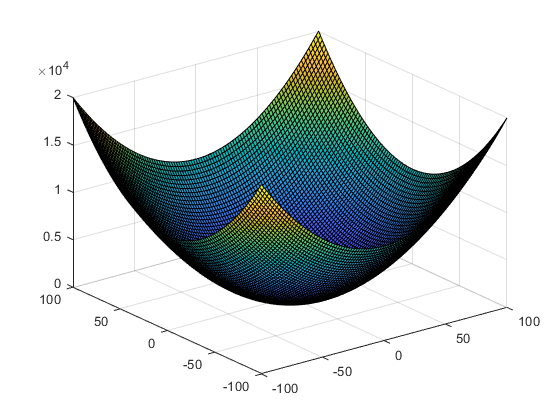
\includegraphics[width=0.6\textwidth]{Images/Control/MPC_Convex_Equation}
\caption{Representation of a convex function plotted using MATLAB.}
\label{convex_function}
\end{figure}

\paragraph{In case of a nonlinear systems} If the system is linearizable, then both Adaptive MPC and Gain-Scheduled MPC can be used in this case. But the constraints are still linear and the cost function is still quadratic. In this case, the nonlinear function can be linearized around an operating point, which will result in a linear function that approximates the nonlinear system well near the operating point. However, it should be noted that the linear function will not work well outside the operating region. This is why it is interesting to find multiple linearized models, with each model representing the nonlinear function well around it's operating point.



\begin{figure}[h]
\centering
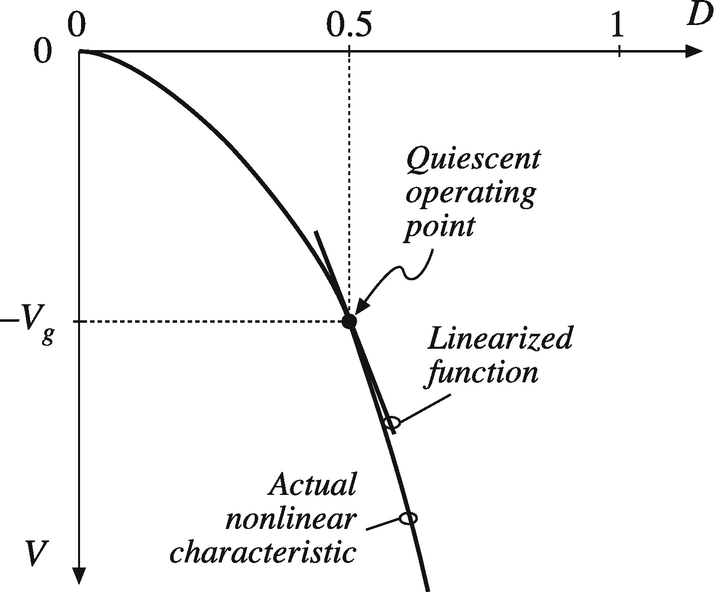
\includegraphics[width=0.45\textwidth]{Images/Control/linearization}
\caption{Example of the linearization of a nonlinear function around an operating point \cite{Erickson2020}.}
\label{nonlinear_function_linearization}
\label{non_convex_function}
\end{figure}



\paragraph{Adaptive MPC} In this case, a linear model is computed on-line as the operating conditions change. And, the internal plant model used by the MPC is updated with the corresponding linear model at each time step. Moreover, it should be noted that the optimization problem remains the same across different operating points. In other words, the number of elements in the state and the constraints remain the same across different operating conditions \cite{Bujarbaruah2018}.

\paragraph{Gain-Scheduled MPC} In this case, linearization of the nonlinear model is done offline at the operating points of interest. Then, a linear MPC controller is designed for each operating point. However, it should be noted that unlike Adaptive MPC, each controller is now independent from the other. In other words, the number of elements in the state and the constraints are different across different operating conditions.
It should also be noted that for this method, an algorithm must be designed to switch between the predefined MPC controllers for different operating conditions. Moreover, Gain-Scheduled MPC also uses more memory than Adaptive MPC \cite{7347864}.

\paragraph{Non-linear MPC} If the system is nonlinear and cannot be linearized, and both the constraints and the cost function are also nonlinear, then Nonlinear MPC can be used in that case. It is the most powerful method of all the different methods mentioned earlier, since it uses the most accurate representation of the plant. Thus, predictions are more accurate. However, Nonlinear MPC is the most difficult method to solve in real-time. Because, in that case the problem becomes a non-convex optimization problem. Thus, the cost function may have many local minima, and finding the global minimum may be hard in that case. An example of a non-convex function is shown in figure \ref{nonconvex_function} below.


\begin{figure}[h]
\centering
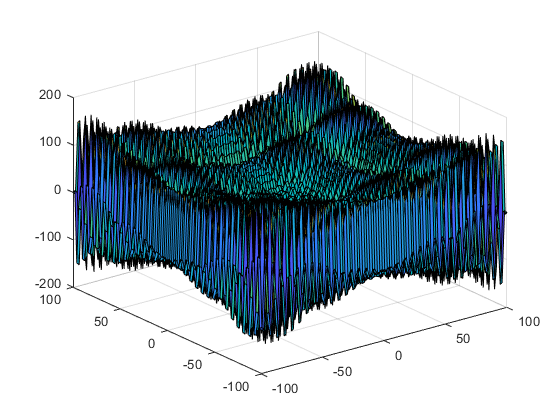
\includegraphics[width=0.6\textwidth]{Images/Control/MPC_Nonconvex_Equation_b}
\caption{Representation of a non-convex function plotted using MATLAB.}
\label{nonconvex_function}
\end{figure}

\newpage

\subsubsection{Strategies to Improve Computational Time}

As demonstrated in (\ref{MPC_problem}), an MPC problem is formulated as a QP problem that tries to minimize a quadratic cost function in general. Moreover, MPC computations become more complex as the number of state elements, the number of constraints and the MPC parameters increase. Moreover, as stated in section \ref{MPC_General_Idea}, if the MPC controller is running on applications with slow dynamics, then computational complexity is not a concern. However, if MPC is running on applications with fast dynamics, then the computational complexity becomes crucial. In addition, it is important to note that the matrices that are stored in the processor of the system for MPC computations grows with the increasing number of optimization variables. Thus, this could cause a memory problem. So, to reduce the complexity and computational time of MPC, the following methods can be used:

\paragraph{Order reduction techniques} They are used to discard states that do not contribute to the dynamics of the system \cite{4421358}. And, using order reduction techniques will also reduce the memory usage of the controller.

\begin{comment}
\paragraph{For applications with small $T_s$} In these cases, the performance of the MPC controller can be increased by \cite{bequette2003process}:
\begin{itemize}
	\item Shortening the prediction horizon.
	\item Shortening the control horizon.
	\item Reducing the number of constraints.
	\item Having lower precision operations and data representation.
\end{itemize} 
It should be noted that for applications with even smaller sample times, \textit{Explicit} MPC can be used.
\end{comment}

\paragraph{Explicit MPC} Instead of solving the optimization problem online for the current state, \textit{Explicit} MPC solves it offline for each value of the state \textbf{\textsc{x}} within a given range \cite{Bemporad2013}. Thus, for each state value within a given range, the Explicit MPC precomputes the optimal solution. And, this solution consists of linear functions that are piecewise affine and continuous is \textbf{\textsc{x}}. An example of Explicit MPC applied on a one-dimensional system is shown in figure \ref{Explicit_MPC_1D} below.

\begin{figure}[h]
\centering
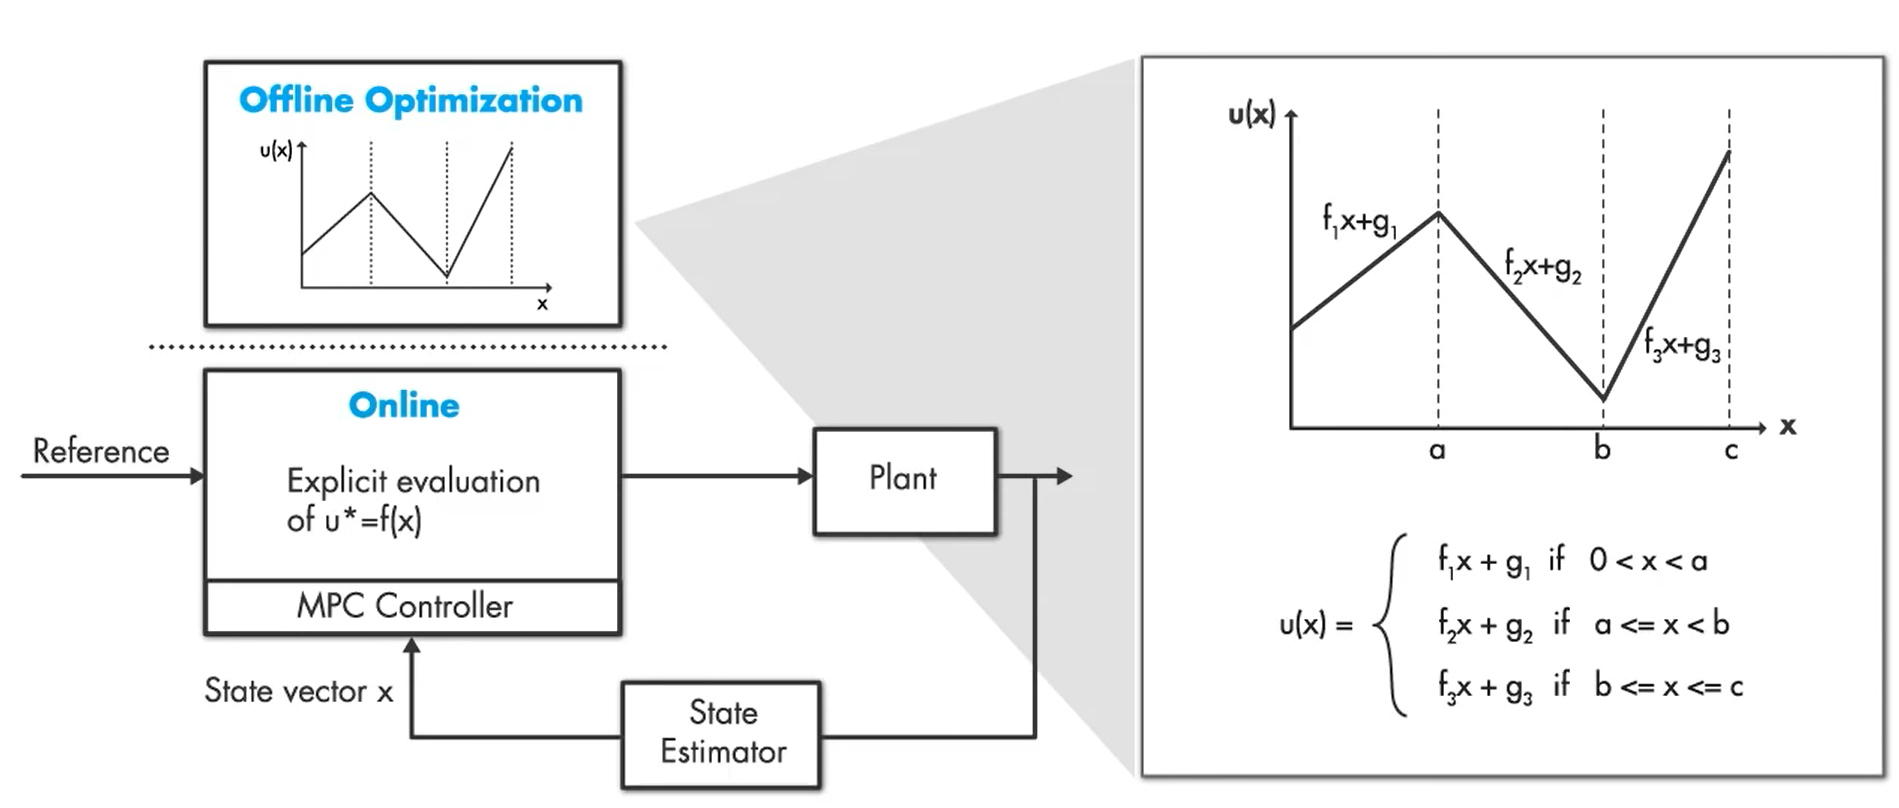
\includegraphics[width=0.9\textwidth]{Images/Control/Explicit_MPC_a}
\caption{Example of an Explicit MPC controller applied on a one-dimensional system \cite{MathWorks2018_new}.}
\label{Explicit_MPC_1D}
\end{figure}

\noindent As can be observed from figure \ref{Explicit_MPC_1D}, the constraints cut the solution space into different regions. And, each region maps into a unique solution.
Another example of an Explicit MPC applied on a two-dimensional system is shown in figure \ref{Explicit_MPC_2D} below. 

\newpage

\begin{figure}[h]
\centering
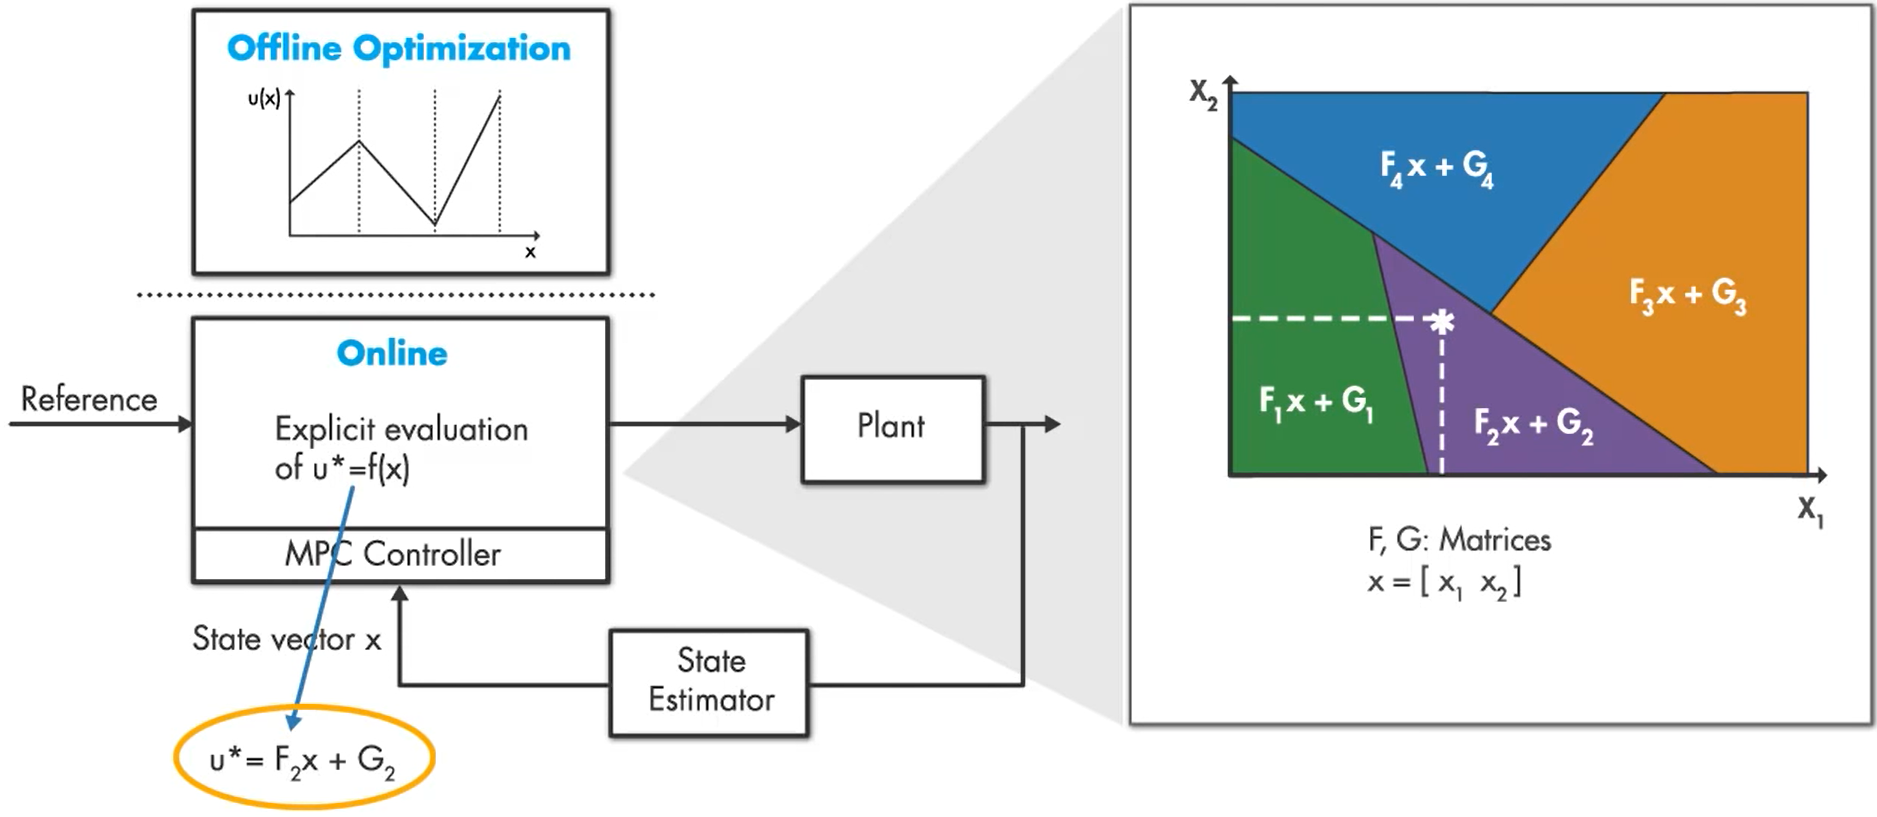
\includegraphics[width=0.9\textwidth]{Images/Control/Explicit_MPC_b}
\caption{Example of an Explicit MPC controller applied on a two-dimensional system \cite{MathWorks2018_new}.}
\label{Explicit_MPC_2D}
\end{figure}

\noindent As can be observed from figure \ref{Explicit_MPC_2D}, the Explicit MPC finds the  region that the current state lies in and evaluates the linear function that creates the current control input.

\noindent Thus, it can be concluded that if the iterative optimization process is reduced to linear function evaluations, then this will greatly simplify the online computations. However, if there is a large number of regions that the state can lie in, then searching for the current state region could sometimes be time consuming. Also, having many regions could cause memory problems for the processor. Thus, the number of regions can be reduced by merging some regions together. However, thee computed solution in that case is not optimal anymore \cite{Hovland2008}.

\paragraph{Suboptimal Solution}
It is another method to improve the computational time of the MPC controller. In a MPC problem, the optimal solution is very unpredictable and can drastically change between each time step. In addition, the computational time may exceed the sample time $T_s$. So, it is mandatory to make sure that a solution can be found within $T_s$ and that there still exists additional time for other tasks that need to be executed \cite{Gulez2014}. A simple example is provided in figure \ref{Suboptimal_solution_example} below where a maximum value for the iterations is determined, and it is taken as 5 for illustration purposes. 


\begin{figure}[h]
\centering
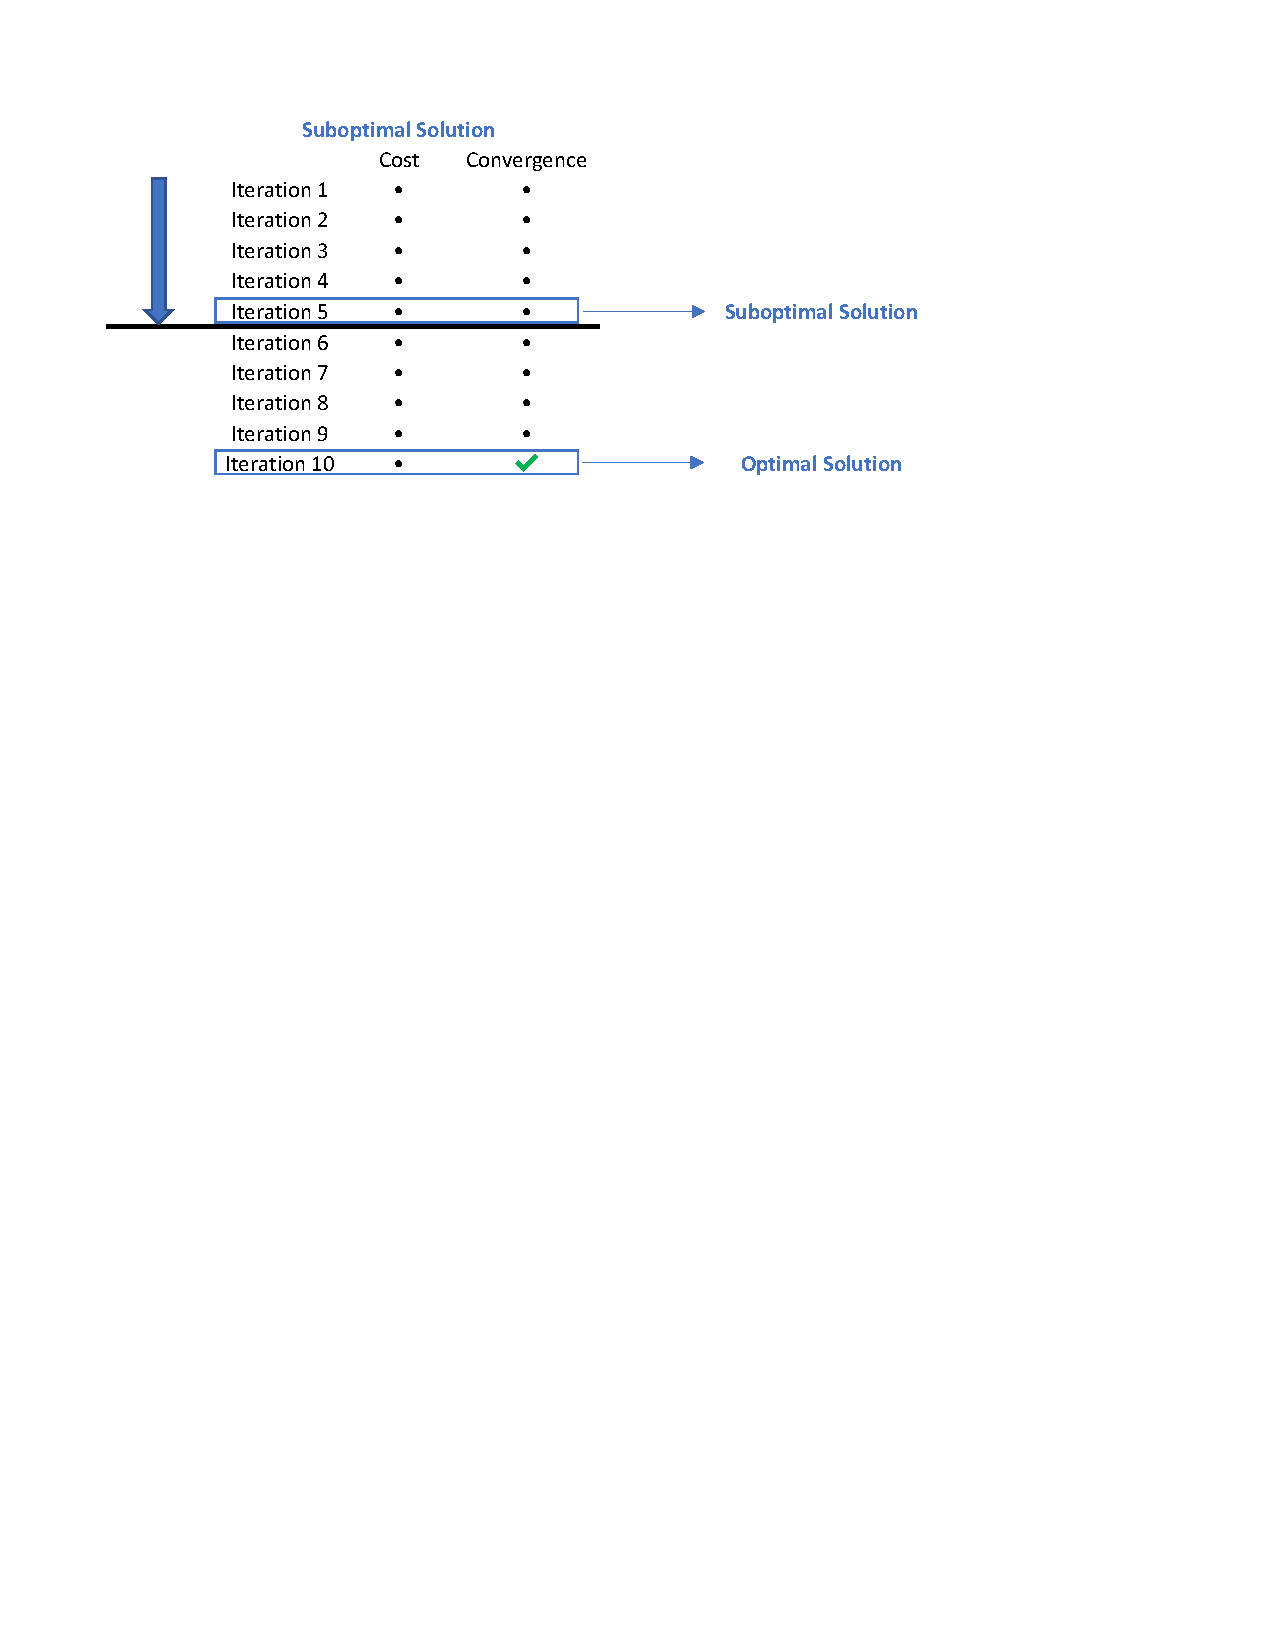
\includegraphics[width=0.8\textwidth]{Images/Control/Suboptimal_Solution.png}
\caption{Example showing how the suboptimal solution is found when the maximum number of iterations is set to 5.}
\label{Suboptimal_solution_example}
\end{figure}

\noindent As can be seen from figure \ref{Suboptimal_solution_example}, the optimal solution is reached in 10 iterations. However, the controller will stop at iteration 5 and take the suboptimal solution. Moreover, it is important to note that the suboptimal solution still satisfies all the constraints of the optimization problem. The only question that remain is how to determine the maximum number of iterations. This can be done by testing the algorithm on the hardware directly and identifying the execution time used by each iteration. Then, the maximum number of iterations is chosen such that the total execution time does not exceed the sample time of the controller.


  \subsubsection{Existing MPC toolboxes} Some of the available tools that allow to solve the MPC problem are listed below.
  
  \begin{itemize}
  	\item \textbf{Model Predictive Control Toolbox}\footnotemark : it is made by MathWorks (closed-source).
  	\item \textbf{MPCtools}\footnotemark : it is a free and open-source toolbox for MATLAB and Simultink that  permits to create and simulate basic MPC controllers by using linear state space models.
  	\item \textbf{do-mpc}\footnotemark : it is a free and comprehensive open-source toolbox for robust model predictive control which is written in Python language.
  	\item \textbf{Control Toolbox}\footnotemark : it is an efficient library for control, estimation, optimization and motion planning in robotics, which is written in C++ language.
  \end{itemize}
  

\footnotetext[1]{\url{https://www.mathworks.com/products/model-predictive-control.html}, accessed on 01/10/2021.}  

\footnotetext[2]{\url{http://www.control.lth.se/research/tools-and-software/mpctools/}, accessed on 01/10/2021.}  

\footnotetext[3]{\url{https://www.do-mpc.com/en/latest/}, accessed on 01/10/2021.}  

\footnotetext[4]{\url{https://github.com/ethz-adrl/control-toolbox}, accessed on 01/10/2021.}  


 \subsection{Sliding mode control}
 
 
 
  \subsubsection{Main Principles}
 
 
 
Sliding mode control (SMC) is a control technique that is nonlinear presenting exceptional attributes of robustness,
accuracy, easy tuning and execution.
 
The aim of SMS systems is to drive the system states to a specific surface in the state space, called  \textit{"sliding surface"}. Upon reaching the sliding surface, sliding mode control allows the states to remain on the close neighborhood of the sliding surface. Therefore, the sliding mode control consists of a controller design with two parts. The first part contains the design of a sliding surface in order for the sliding motion to fulfill design requirements. The second deals with selecting a control law that makes the switching surface interesting with respect to the system state \cite{Utkin1997}.

There exists two main benefits of sliding mode control. Firstly, the behavior of the dynamics of the system can be changed according to a specific selection of the sliding function. Secondly, the response of the closed loop system becomes completely insensitive to some special uncertainties. This principle goes beyond bounded model parameter uncertainties, interference and non-linearity. In a practical sense, SMC allows the control of nonlinear processes that are affected by external noise and heavy model uncertainties.

The most important principles of SMC are shown in the following significant references \cite{Utkin1997,DeCarlo1998,Hung1993}. Researchers have also studied the problems appearing in the practical execution of this class of techniques. \cite{Young1999}

Moreover, the book \cite{Bartolini2008} presents a very modern overview of the most promising current line of theoretical and practical research in the domain.

 
 \subsubsection{Simple Description}
 
 Considereing the SISO nonlinear system:
 
 \begin{align}
 \dot{x} &=f(x,t)+g(x,t)u \label{SISO_1}\\
 y &= h(x,t) \label{SISO_2}
 \end{align}


Where y and u represent the scalar output and input variable, and $x \in \mathbb{R}^n$ represents the state vector.



The goal of the control is to make the output variable y follow a chosen profile $y_{DES}$. This means that it is needed that the
output error variable $e=y-y_{DES}$ tend to a small proximity of zero following a transient of reasonable duration.


As stated earlier, the synthesis of SMC requires two phases:

\begin{itemize}
	\item [] \textbf{Phase 1}: \textit{"Sliding Surface Design"}.
	\item [] \textbf{Phase 2}: \textit{"Control Input Design"}
\end{itemize}


In the first phase, a specific scalar function $\sigma$ of the system state is defined such that:

\begin{equation*}
	\sigma({\textsc{x}}):\mathbb{R}^n \rightarrow \mathbb{R}.
\end{equation*}


In many cases, the sliding surface relies on the tracking error $e_y$, along with a specific number of its derivatives

\begin{equation}
	\sigma = \sigma(e,\dot{e},\ldots,e^{(k)})
\end{equation}


The function $\sigma$ must be chosen in a way that when $\sigma=0$, it will result in a stable differential equation such that any $e_y(t) \rightarrow 0$ as $t \rightarrow \infty$.


The most common choices for the sliding manifold are the following:

\begin{align}
\sigma = \dot{e} + c_0 e\\
\sigma = \ddot{e} + c_1 \dot{e} + c_0 e \\
\sigma = e^{(k)} + \sum_{i=0}^{k-1} c_i e^{(i)}\label{equation_with_k}
\end{align} 



The number of derivatives that should be included ( $k$ in (\ref{equation_with_k})) must be $k=r-1$, where $r$ is the input-output relative
degree of  (\ref{SISO_1})-(\ref{SISO_2}).


With correctly chosen $c_i$ coefficients, if $\sigma$ is driven to 0, then the error and its derivatives will decrease to 0 exponentially.



Provided that such property holds, the goal of the  control system is to drive $\sigma$ to 0.


From a geometrical perspective, the equation $\sigma=0$ represents a surface in the error space that is called \textit{"sliding surface"}. The trajectories of the system that is being controlled are forced to be on the sliding surface, along which the behavior of the system satisfies the design requirements.


A common form for the sliding surface depends on a  scalar parameter $p$, and is expressed as follows:

\begin{equation}
\sigma = \bigg(\frac{d}{dt}+p\bigg)^k e
\end{equation}

\begin{align}
k&=1 \text{\hspace{0.5cm}} \sigma = \dot{e} + pe \\
k&=2 \text{\hspace{0.5cm}} \sigma = \ddot{e} + 2p \dot{e} + p^2 e
\end{align}
 
\noindent The parameter p can be chosen randomly, and it defines the particular pole of the derived \textit{"reduced dynamics"} of the system when sliding.
 

\noindent The integer parameter $k$ is on the other hand somewhat crucial, it is required be equal to $r-1$, and $r$ should be the relative
degree between y and u. This signifies that the relative degree of the $\sigma$ variable is one.


\noindent The next phase (\textbf{Phase 2 }) is about determining a control action that guides the trajectories of the system onto the sliding manifol. This means that the control is capable of driving the $\sigma$ variable to zero in finite time.


\noindent There exist many approaches that are based on the approach of sliding mode control:

\begin{itemize}
	\item \textit{"Standard"} ( also called \textit{"first-order"}) sliding mode control.
	\item \textit{"High-order"} sliding mode control.
\end{itemize}


Focus is devoted to the second order sliding mode method, and a few references to the higher order approaches
are also granted. Frequent characteristic of all sliding mode-based techniques is that no specific information about the
original system dynamics is required. In other words, the controlled system will be treated as an entirely uncertain “black box” object.



\subsubsection{First-Order Sliding Mode Control}


Along the manifold $\sigma=0$, the control is discontinuous. So, it can be expressed as follows:

\begin{equation}
	u = -U \space sgn(\sigma)
\end{equation}


This means that:

\begin{equation}
\begin{aligned}
	u = \begin{cases}
		-U \hspace{0.5cm} &\sigma>0 \\
		U \hspace{0.5cm}  &\sigma<0
	\end{cases}
\end{aligned}
\end{equation}

With $U$ having a constant, positive and sufficiently large value.

\begin{figure}[h]
\centering
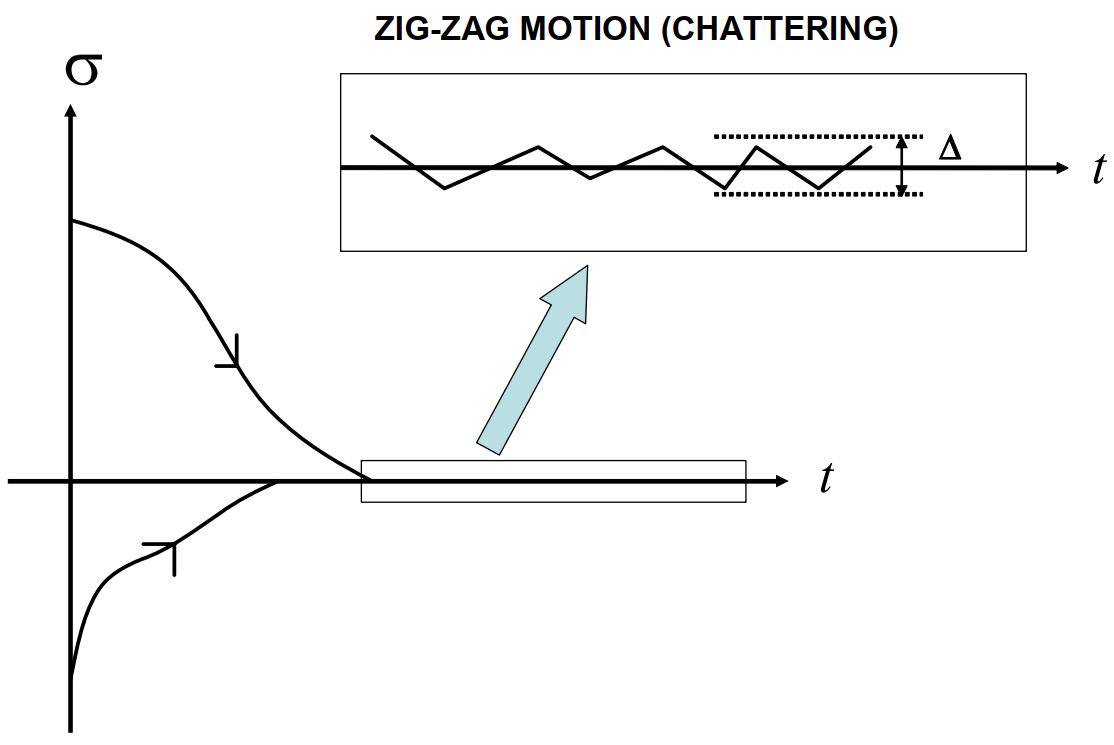
\includegraphics[width=0.6\textwidth]{Images/Control/first_order_sliding_mode_control}
\caption{Typical evolution of $\sigma$ starting from different initial conditions. \cite{DeCarlo2008}}
\label{sigma_evolution}
\end{figure}

\newpage

\begin{figure}[h]
\centering
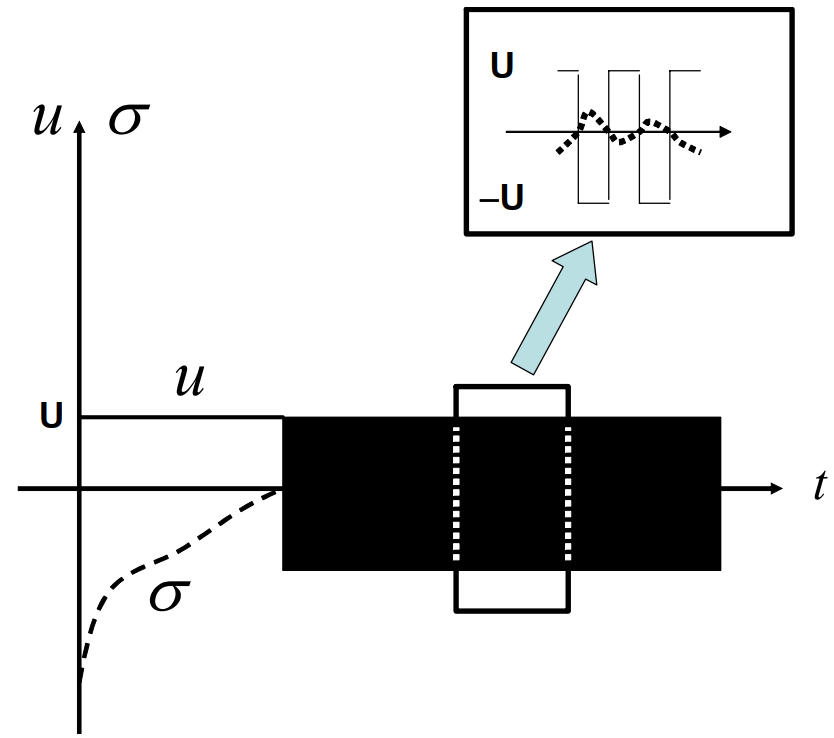
\includegraphics[width=0.5\textwidth]{Images/Control/first_order_sliding_mode_control_b}
\caption{Typical evolution of the control signal $u$ ( $\sigma$ is represented by dashed lines). \cite{DeCarlo2008}}
\label{control_evolution}
\end{figure}


\noindent In steady condition the control variable u will alternate at very high (theoretically infinite) frequency along the values u=U
and u=-U, which can be observed in figure \ref{control_evolution}.



\noindent The discontinuous switching control with high frequency  in figure \ref{control_evolution} is suitable in electrical implementations (where PWM control signals are usually used) but it results in an increase in oscillations and numerous different problems in several areas, such as the control of mechanical systems.


In order to find a solution for the problem presented above (referred to as \textit{”chattering phenomenon”}) roughly (smoothed) execution of sliding mode control techniques have been proposed where the discontinuous \textit{“sign”} term is substituted with a  continuous and smooth estimation using any of the two functions below.


\begin{equation}
\begin{aligned}
&\text{SAT} \text{\hspace{1cm}} u=-U sat(\sigma; \epsilon) \equiv -U \frac{\sigma}{|\sigma| + \sigma} \text{\hspace{1.5cm}} \epsilon >0 \text{\hspace{0.5cm}} \epsilon \approx 0 \\
&\text{TANH} \text{\hspace{1cm}} u=-U tanh(\sigma/ \epsilon)  \text{\hspace{3.3cm}} \epsilon >0 \text{\hspace{0.5cm}} \epsilon \approx 0  \\
\end{aligned}
\end{equation}

Unfortunately, this approach is successful only when uncertainties are not applied on the system and the control action that prevents these uncertainties can be set to zero in the sliding mode.


\begin{figure}[h]
\centering
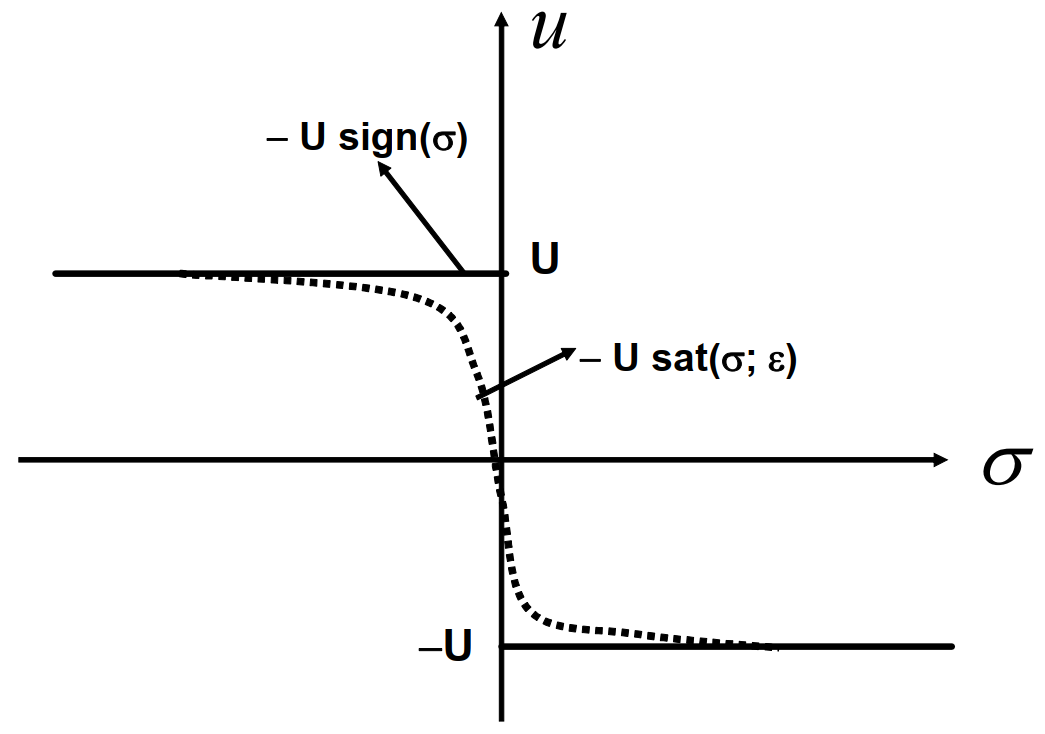
\includegraphics[width=0.6\textwidth]{Images/Control/first_order_sliding_mode_control_c}
\caption{Smooth approximations of sliding mode control. \cite{DeCarlo2008}}
\label{Smooth_Sliding_mode_control}
\end{figure}

\subsubsection{Second order sliding mode control}


By using the above-described smooth approximations, some problems will be reduced. However, this comes at the expense of a loss of robustness.


Second order sliding mode control algorithms are effective approaches that entirely resolve the chattering problem without compromising the properties of robustness.


There has been many studies on second order sliding mode control. Two of the most interesting papers are \cite{Levant1993, Bartolini1999}. An overview of the mentioned papers is shown below.


\paragraph{SuperTwisting Algorithm}

It is of the most used (2-SMC) algorithms. This algorithm is expressed with the following equations:

\begin{equation}
\begin{aligned}
	u &= \lambda \sqrt{|\sigma|}sign(\sigma) + w \\
	\dot{w} &= -W sign (\sigma) \\
\end{aligned}
\end{equation}


									
An appropriate way for tuning its parameters is by using the following relations: 

\begin{equation}
\lambda = \sqrt{U} \text{\hspace{2cm}} W = 1.1U
\end{equation}



\noindent With $U$ being a positive constant that should be taken sufficiently large.



\noindent Practically, one has to gradually increase U until good performance is attained in the closed loop system. This type of single-parameter \textit{“trial and error”} tuning is specifically suitable in practical applications.

\noindent The super-twisting algorithm can be considered to be a nonlinear version of a classical PI controller. This correlation becomes clear by referring to figure \ref{PI_SuperTwisting} below.

\begin{figure}[h]
\centering
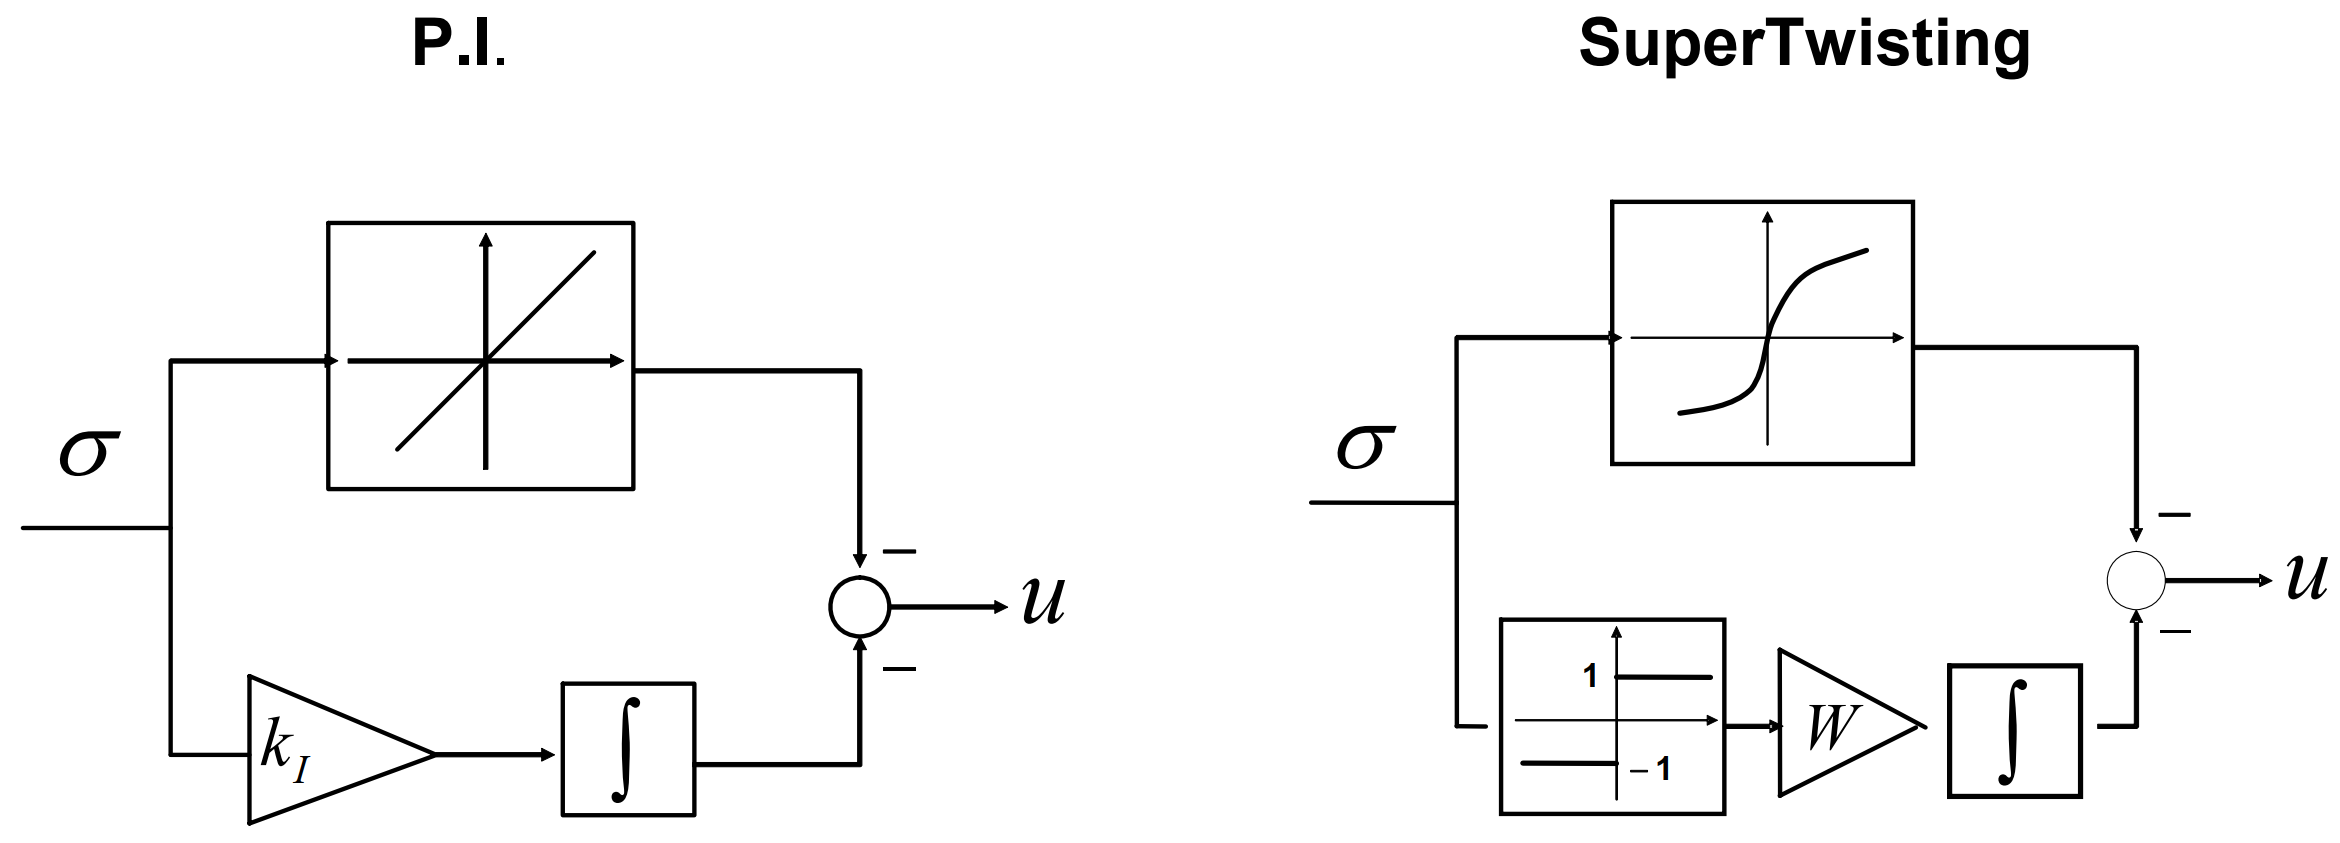
\includegraphics[width=\textwidth]{Images/Control/PI_SuperTwisting}
\caption{Block diagrams of a PI (left) and Super-Twisting (right) controllers.\cite{DeCarlo2008}}
\label{PI_SuperTwisting}
\end{figure}



\noindent Second order SMC resolves the chattering problem because the control law is now a continuous function of time. 
In the sight of dynamics that are not modeled, some remaining chattering exist. But there are some design methods to second-order modes that can limit such an aspect which is not desired.

\newpage

 \subsection{Other Types of Nonlinear Control Methods}
 
Although the approaches that have been mentioned so far are potentially useful for this master thesis, there is still some other approaches that deserve to be mentioned because of their popularity and applications:


\begin{itemize}
\setlength{\itemindent}{-.5in}
	\item [] \textbf{Backstepping control} The main idea is to divide the system into successive subsystems and to apply a recursive algorithm which will stabilize each subsystem after the other \cite{Madani2006}. However, this method is not robust, but it is computationally fast. In order to handle disturbances, Fang et al. \cite{Gao2011} implemented an integral backstepping control law, in which the integral term was shown to reduce steady state errors and the response time of the system greatly. 

	\item [] \textbf{Adaptive control} This method is required when the parameters that are characterizing the system contain errors or are unknown. This type of control algorithms contains a parameter adaptation law, which is enclosed in the control to track the desired trajectory of the system, even if the model of the system is not completely known.
For instance, Diao et al. \cite{Diao2011} obtained good performance even though the inertial parameters of the quadrotor and the aerodynamic coefficients were not perfectly known.
This method is convenient in some cases. such as the existence of unpredictable wind \cite{Antonelli2013} or pick-and-place applications with small loads. 
	 
 \end{itemize}
 
\noindent Moreover, other methods for the control of quadrotors could be found  in the next chapter, where the state of the art in the performance of flipping maneuvers with quadrotors is provided. 
 
 
 \chapter{Multi-flips maneuver with quadrotors}


The aim of this chapter is to explain the physics of the multi-flip maneuver, in addition to the major difficulties that relate to the implementation of flipping maneuvers with quadrotors. Furthermore, a review of the existing limitations that the current approaches have are shown and the existing scientific literature is presented. The content of this chapter were thoroughly covered by the previous master students Marco Orsingher and Antonio Marino for which their papers were used as references for this chapter. In fact, Orsingher \cite{Orsingher2019} managed to perform the flipping maneuver in simulations on MATLAB and ROS by using polynomial trajectory generation techniques, however real experiments were unsuccessful. Marino \cite{Marino2020} tackled the same problem the very next year by using trajectory optimization techniques. After successful simulations in ROS, Marino was able to perform a single flip in real experimentation. However, due to the pandemic, no further experiments were possible.


\section{Physics of a quadrotor flip}\label{multiflip_physics}


In order to perform the tedious process of multi-flip maneuvers with a quadrotor, high angular velocity and large angle attitude control are needed. More conventionally, the multi-flip trajectory can be expressed as a rotation of $2n \pi$ about a flipping axis \textbf{a}, with n the number of desired flips to be carried out by the quadrotor. Physically, the maneuver can be divided into 4 different phases, which are shown in figure \ref{flipping_physics}.

\begin{itemize}
\setlength{\itemindent}{-.5in}
	\item [] \textbf{Climb phase} The quadrotor must accelerate in a vertical direction as much as possible. This will ensure that the required height to perform the multi-flip maneuver is achieved. In fact, while performing the multi-flip maneuver, the thrust forces cannot balance out the weight of the drone. This will cause the drone to start falling. The duration of this phase is based on the number of flips that must be performed by the quadrotor. This number will be chosen by the user.

	\item[] \textbf{Multi-flip phase} This stage begins the moment the vehicle starts rotating and continues until the flipping angle reaches the chosen value of $2n \pi$. In this phase, the quadrotor hits the maximum altitude because of the required high angular velocity and starts falling because of the gravity effect. Generally, all the focus is on following the desired closed-loop attitude, and the vertical position is not controlled. the time spent in this phase depends on the desired number of flips $n$ and on the maximum angular velocity achievable by the quadrotor.
	
	\item [] \textbf{Descent phase} In order for the quadrotor not to crash into the ground, the main idea is to set the maximum thrust reference to the actuation system. This will balance out the gravity force. The higher the number of required flips, the faster the quadrotor will fall due to gravity effects. Thus, this phase ends when the descent is fully balanced out. The user may also decide what the duration of this phase is if the physics of the problem allow a slower descent.
	\item [] \textbf{Re-stabilization phase} In this phase, the altitude of the quadrotor is adjusted to a desired value. Moreover, this phase ends when a new control signal is provided by the user. 
\end{itemize}

\begin{figure}[h]
\centering
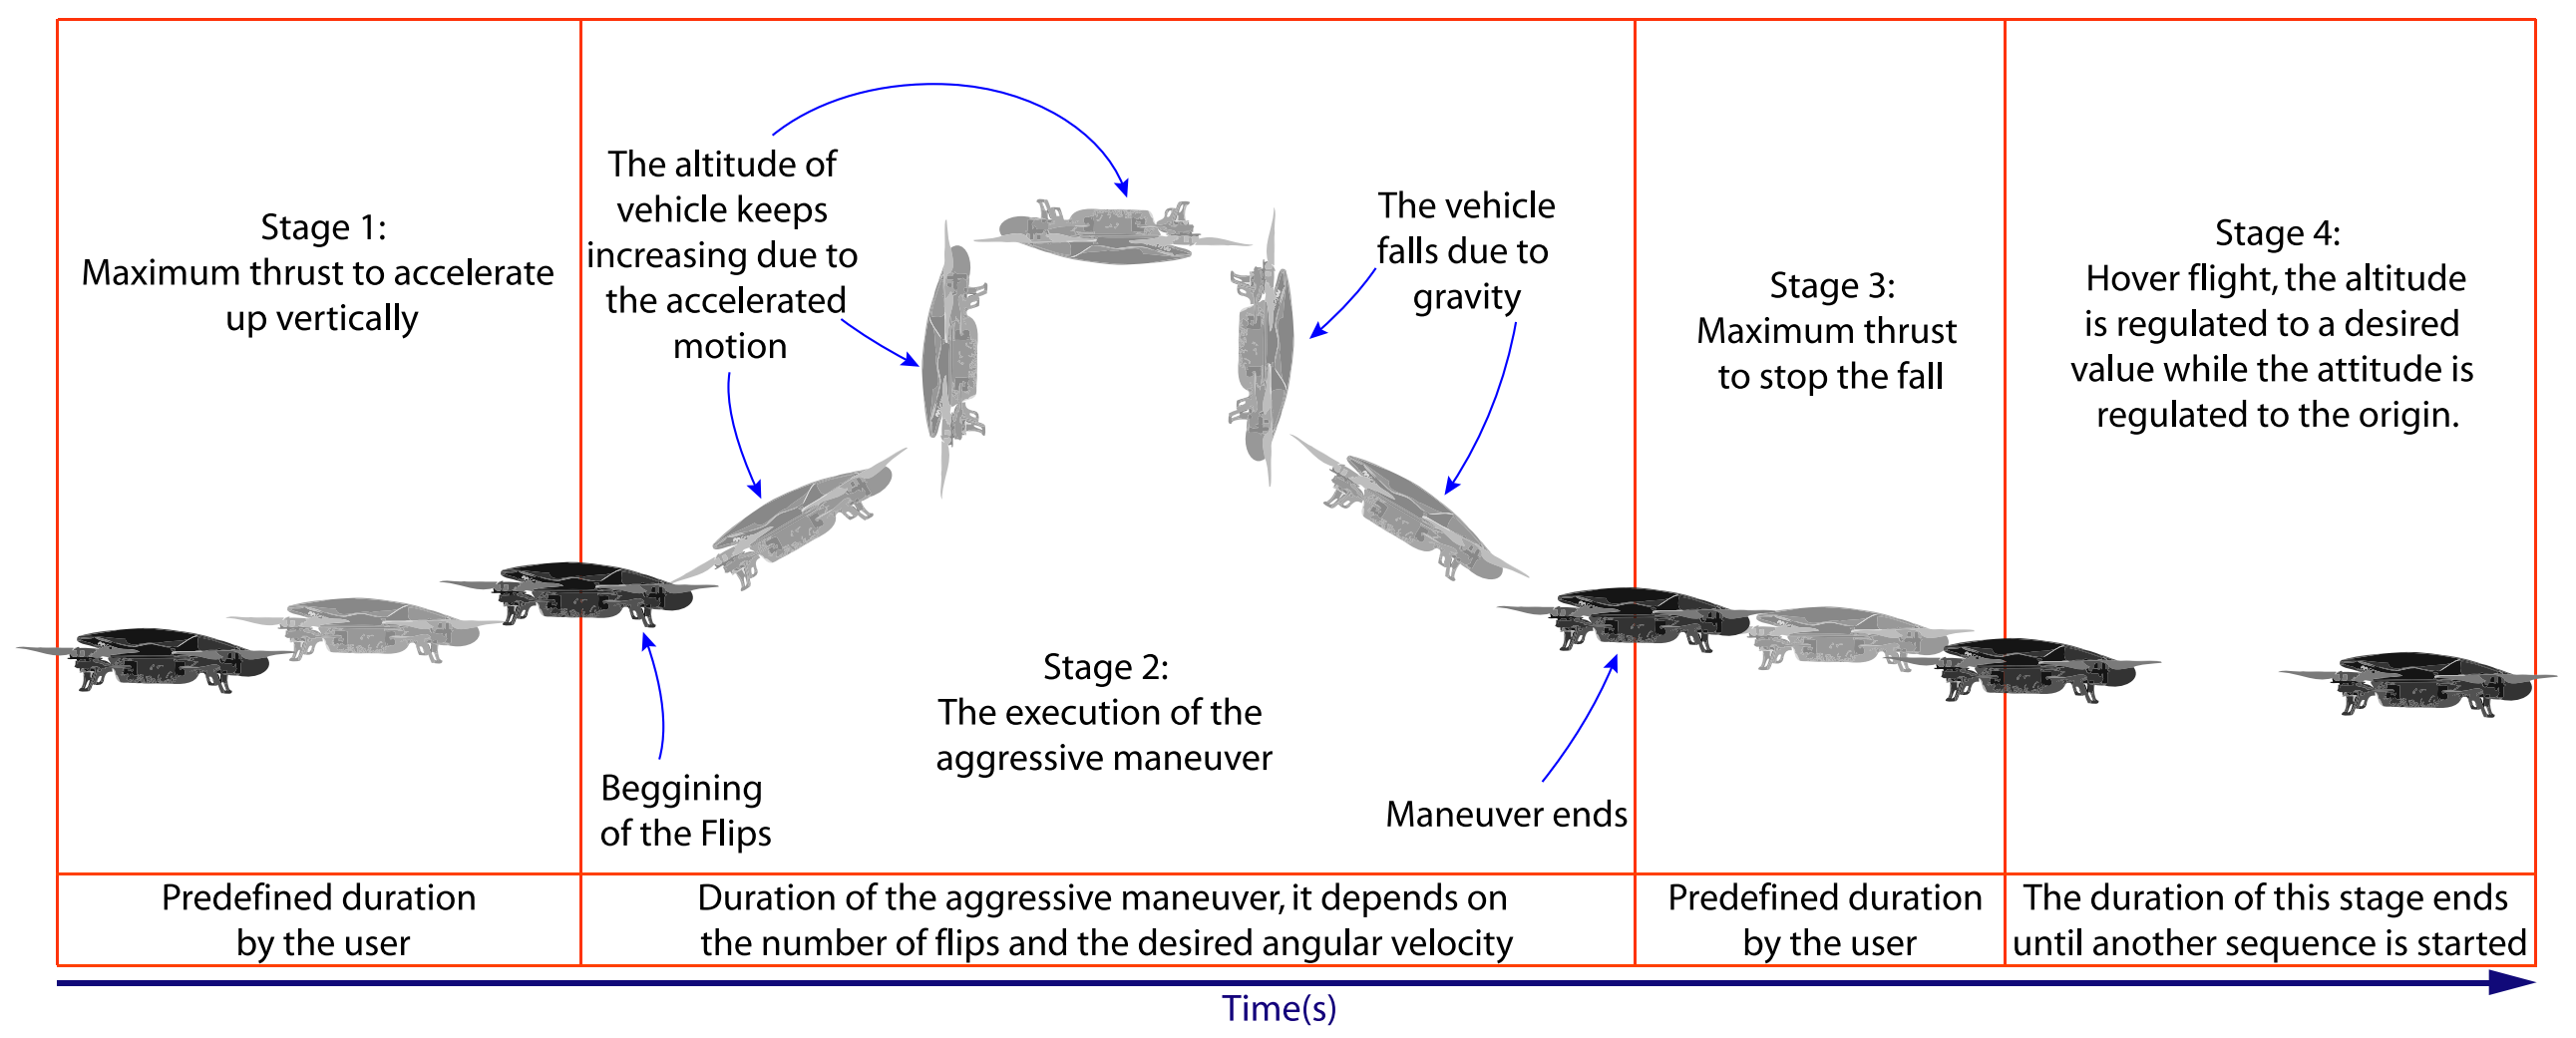
\includegraphics[width=0.7\textwidth]{Images/Flip/Physics}
\caption{Representation of the different phases needed for performing multi-flip maneuvers\cite{Castillo2018}.}
\label{flipping_physics}
\end{figure}


 \section{Control Approaches for Multi-Flip Maneuvers}
 
The research community has tackled the multi-flip problem numerous times on quadrotors and different methods have been suggested to achieve up to triple flips both indoor and outdoor. The existing research can be stored into three different methods: hybrid systems theory, open-loop iterative learning and closed-loop attitude control. This section gives an inclusive overview and suitable references on the state of the art in flipping maneuvers with quadrotors.
  
 \subsection{Hybrid Systems Theory}
 
A convenient approach for dealing with complex systems is to divide them into a set of individual modes. Each mode will have its own continuous dynamics equations. Then, they will be analyzed by using hybrid systems theory. Gillula et al. (\cite{Gillula2011,Gillula2010}) suggested using this strategy for quadrotor multi-flips. The main idea is to breakdown the flipping maneuver into a sequence of individual phases and then use an appropriate technique from hybrid systems theory to generate provable transitions between the modes. By doing this procedure, the maneuver will be able to be performed safely. The separate modes that are considered in this work are shown in figure \ref{hybrid_systems_theory_figure}, which should be right from right to left. When compared to the different phases shown in section \ref{multiflip_physics}, the climb phase is called the \textit{"impulse"}, the multi-flip phase is the \textit{"drift"} and the descent and the re-stabilization phases are merged together and are called \textit{"recovery"}.
 
 \begin{figure}[h]
 \centering
 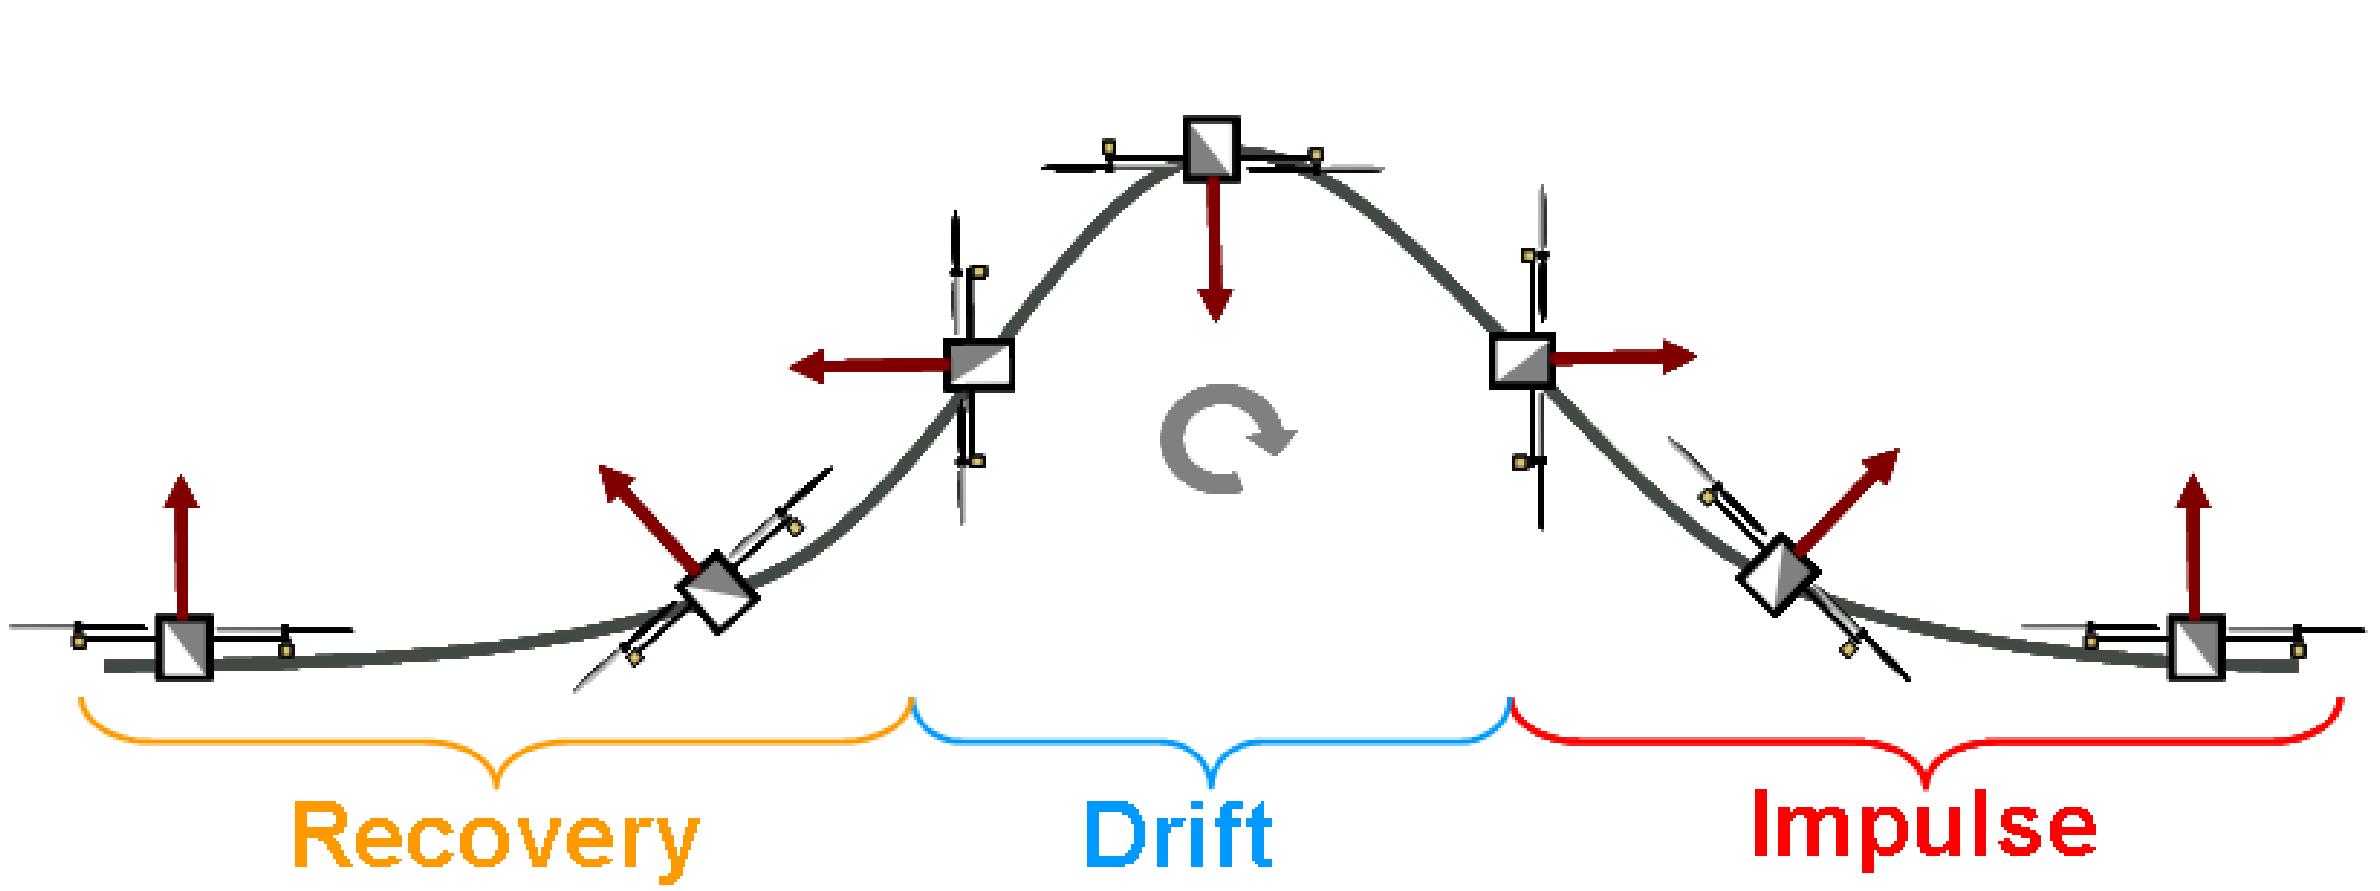
\includegraphics[width=\textwidth]{Images/Flip/Hybrid_Systems_Theory}
 \caption{Representation of the individual phases during a backlip (from right to left)\cite{Gillula2011}}
 \label{hybrid_systems_theory_figure}
 \end{figure}

\newpage

\noindent The tool used for generating feasible transitions between the individual modes is called the \textit{"theory of reachable sets"}. By considering a system characterized by the following dynamics: 

\begin{equation}
	\dot{\textbf{\textsc{x}}}=  \textbf{\textsc{f}} ( \textbf{\textsc{x}}, \textbf{\textsc{u}}, \textbf{\textsc{d}})
\end{equation}


with $\textbf{\textsc{x}}$ the state of the system, $\textbf{\textsc{u}} \in U$ the control input of the system and $\textbf{\textsc{d}} \in D$ a bounded noise applied on the system. In that case, two different types of reachable sets are established:

\begin{enumerate}
	\item A \textit{capture set} which represents all the states for which, for any possible value of the noise $\textbf{\textsc{d}}$, the control input $\textbf{\textsc{u}}$ is still capable of driving the state into a desired state region in a finite time horizon $t$.
	\item An \textit{avoid set} which represents all the states for which, for any possible value of the control input $\textbf{\textsc{u}}$, the noise $\textbf{\textsc{d}}$ will drive the system into an undesired set. Thus, the roles of $\textbf{\textsc{u}}$ and $\textbf{\textsc{d}}$ are reversed when compared to the capture set.
\end{enumerate}

\noindent Generating quadrotor maneuvers using reachable sets is achievable by using a backward approach. The main idea consists of starting from the final desired set, the dynamics of the $n$-th mode can be run in reverse to build a capture set for that phase. This capture set becomes the target region for the $(n-1)$-th node and the procedure will be repeated between every 2 modes. By applying this procedure, feasible transitions between a chain of individual modes can be built. From a mathematical perspective, the problem is formulated as a differential battle between the control and the noise.
In fact, the aim of the control input $\textbf{\textsc{u}}$ is to keep the state of the system away from the region of undesired sets which the noise $\textbf{\textsc{d}}$ is attempting to drive the state of system into (\textit{avoid set}) and also to reach a desired set. Whereas the noise attempts to drive the state of the system out of it (\textit{capture set}). This method has been proven to be successful with a 1.1 kg quadrotor which was able to perform a backflip outdoors. However, the main disadvantage of this method is that it necessitates a long procedure of generating such capture sets and avoid sets. 


\subsection{Open-Loop Iterative Learning}

One of the main issues that is related to performing aggressive maneuvers with quadrotors is that having an exact physical modeling of the quadrotor during an intense flight procedure is very complicated. In addition, generating reference trajectories for aerobatic flight is not an easy operation. Beginning from these factors, Lupashin et al. (\cite{Lupashin2010,Lupashin2011,Lupashin2012})
designed a simple open-loop iterative learning method to perform multi-flip maneuvers without performing any aerodynamic modeling nor trajectory planning. The workflow of this method is shown in figure \ref{Open_Loop_iterative_Learning} on the left.



\begin{figure}[h]
     \centering
     \begin{subfigure}[b]{0.45\textwidth}
         \centering
         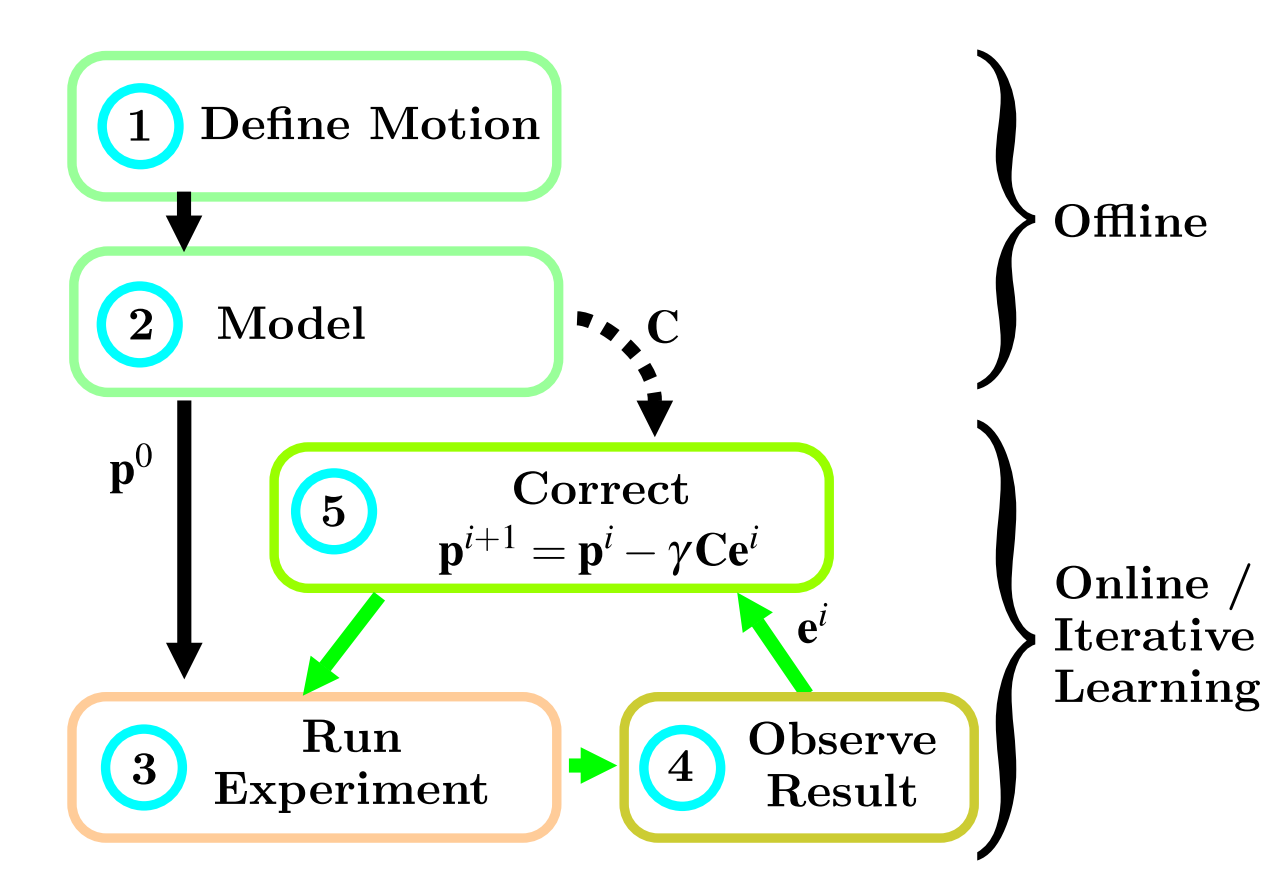
\includegraphics[width=\textwidth]{Images/Flip/Open_Loop_iterative_learning_a}
         \caption{The global workflow of the algorithm}
         \label{fig:Open_Loop_a}
     \end{subfigure}
     \hfill
     \begin{subfigure}[b]{0.45\textwidth}
         \centering
         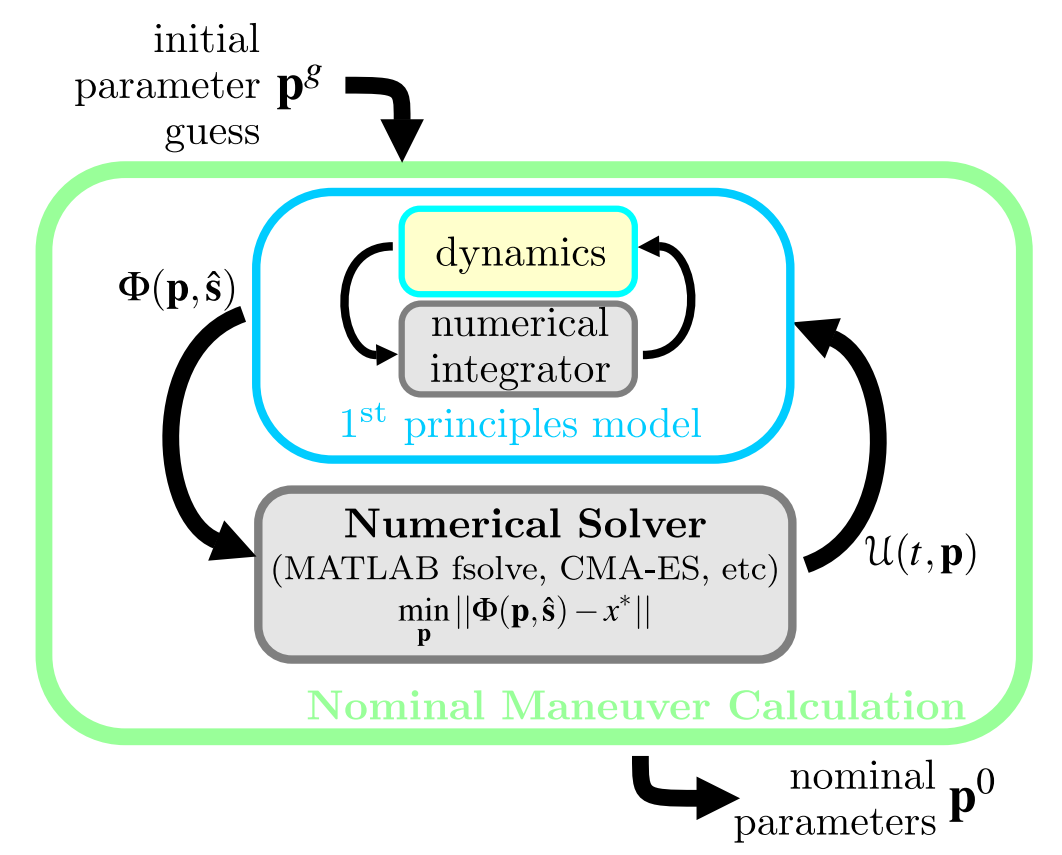
\includegraphics[width=\textwidth]{Images/Flip/Open_Loop_iterative_learning_b}
         \caption{The global workflow of the algorithm}
         \label{fig:Open_Loop_b}
     \end{subfigure}
        \caption{The open-loop iterative learning workflow for performing multi-flips with quadrotors\cite{Lupashin2012}.}
        \label{Open_Loop_iterative_Learning}
\end{figure}

\noindent The first step which is needed is to determine the desired motion in a parameterized manner, so that it is possible to optimize vector $\textbf{\textsc{p}}$ over such parameters. $\textbf{\textsc{p}}$ contains the time and the accelerations needed during each phase of the flip maneuver.  The second procedure which is needed to initialize the iterative learning algorithm is to calculate the nominal motion and to build the correction matrix. Starting from a simplified model of the quadrotor and a coarse initial guess $\textbf{\textsc{p}}^g$, then a numerical solver is utilized to calculate the nominal parameters $\textbf{\textsc{p}}^0$ in order to execute the multi-flip maneuver. In fact, assuming that the desired final state $\textbf{\textsc{x}}^{*}$ can be attained with the control input $\textbf{\textsc{u}}(\textbf{\textsc{p}},t)$ and by referring to $\bm{\Phi}(\textbf{\textsc{p}},\hat{\textbf{\textsc{s}}})$ as the final state of the nominal system after the maneuver is executed.(with the vector $\hat{\textbf{\textsc{s}}}$ representing physical constants), then the nominal set of parameters $\textbf{\textsc{p}}^0$ is the solution of the following optimization problem, as shown in figure \ref{Open_Loop_iterative_Learning}:

\begin{equation}
	\textbf{\textsc{p}}^0 = \text{arg}\min \|\bm{\Phi}(\textbf{\textsc{p}},\hat{\textbf{\textsc{s}}})-\textbf{\textsc{x}}^{*}\|
\end{equation}


\noindent Moreover, by denoting $\bm{\Phi}(\textbf{\textsc{p}}^0,\hat{\textbf{\textsc{s}}})$ as the final state of the nominal model obtained using the nominal set of parameters calculated earlier, then the correction matrix for the iterative learning algorithm is expressed as follows:

\begin{equation}
	\bm{C}=\bigg(\frac{\partial \bm{\Phi}(\textbf{\textsc{p}}^0,\hat{\textbf{\textsc{s}}})}{\partial \textbf{\textsc{p}}}\bigg)^{-1}
\end{equation}

\noindent In the end, steps 3 to 5 in figure \ref{fig:Open_Loop_a} will then run online in an iterative manner until a proposed convergence criterion is satisfied. For $i=0 \ldots n$, the motion is carried out on the quadrotor itself while using the current set of parameters $\textbf{\textsc{p}}^i$ and the final measured error $\textbf{\textsc{e}}^i$. Subsequently, the parameters are updated according to the following law: 

\begin{equation}
\textbf{\textsc{p}}^{i+1} = \textbf{\textsc{p}}^i - \gamma \textbf{\textsc{C}}\textbf{\textsc{e}}^i
\end{equation}

with $\gamma$ being a step size which is defined by the user. This method is very simple does not require complex computations. But, it is by definition an open-loop method. Thus, there are no guarantees that the maneuver will be performed successfully. In fact, a triple flip maneuver has been done during experiments with this method, however the repeatability of this result is a big problem. In addition, "creating a parameterized input trajectory formulation that results in a robust learning strategy remains a difficult and tedious task" \cite{Lupashin2012}.


 
 \subsection{Closed-Loop Attitude Control}
 
 The most known strategy for obtaining great results in flipping maneuvers of quadrotors is to use closed-loop control just for the attitude part of the platform, thus the position of the center of mass during the flipping maneuver is ignored. Many research works can be recognized under this context, and all of them follow the same ideology: a proper reference on attitude or angular velocity is planned and then tracked in closed-loop with a nonlinear control law. Each paper is distinguished from the others based on the strategy that is chosen to build the control law: attractive ellipsoid method \cite{Castillo2018}, geometric control \cite{Lee2010},  energy-based control\cite{Badawy2016} , direct Lyapunov method \cite{Wang2014}.
Particularly, Chen et al. (\cite{Chen2016}, \cite{Chen2017} ,\cite{Chen2018}) generated interesting series of papers  within this framework that should be mentioned because they applied the method on the same physical platform of this thesis (Crazyflie 2.0); moreover, significant theoretical contributions have been provided in these papers to greatly comprehend the issue of quadrotor flipping. Particularly, three elements have been investigated:

\begin{enumerate}
	\item A new depiction of the flipping angle, called $\phi_g$, such that a flip around a random axis $\textbf{\textsc{a}}$ through the center of mass of the quadrotor can be determined. This has permitted to execute multiple flips about the body-fixed axis $\textbf{\textsc{b}}_1$, and another general axis, rotated by $45 ^{\circ}$ on the ($\textbf{\textsc{b}}_1$,$\textbf{\textsc{b}}_2$) plane.
	\item A meticulous angular speed planning approach using cubic splines to produce the reference signal $\bm{\omega}_d$ in such a way that the dynamics of actuation are respected by ensuring that $w_{max}$ is never surpassed. Particularly, the reference is made out of three distinct stages, corresponding to the physical stages presented in figure \ref{closed_loop_a}. In fact, throughout the \textit{climb phase} a rising-speed section  $\bm{\omega}_{d,1}$ is needed to reach  $\bm{\omega}_{max}$, then a stage of constant-speed at  $\bm{\omega}_{d,2}= \bm{\omega}_{max}$ is held while the quadrotor is flipping (\textit{multi-flip phase}), and in the end, the angular velocity $\bm{\omega}_{d,3}$ is reduced to zero within the \textit{descent} and \textit{re-stabilization phase}. The use of cubic functions ensures that the angular accelerations is kept continuous during all the process. Other works, such as \cite{Castillo2018}, suggested equivalent shape, however linear functions were used instead of splines. Considering that the time derivative of a linear function is just a constant, this resulted in undesirable jumps in the angular reference.\\
Considering the desired number of rotations accumulated with each stage $\Phi_{g,i}1$, the time of each stage is changed based on the current flipping angle $\phi_g$:

\begin{equation}
	\bm{\omega}_d(t) = \begin{cases}
	\bm{\omega}_{d,1} \text{\hspace{0.5cm} if \hspace{0.5cm}} \phi_g \leq \Phi_{g,1} \\
	\bm{\omega}_{d,2} \text{\hspace{0.5cm} if \hspace{0.5cm}} \Phi_{g,1} < \phi_g \leq \Phi_{g,1} + \Phi_{g,2} \\
	\bm{\omega}_{d,3} \text{\hspace{0.5cm} if \hspace{0.5cm}} \Phi_{g,1} + \Phi_{g,2} < \phi_g \leq \Phi_{g,1} + \Phi_{g,2} + \Phi_{g,3} \\
	\end{cases} 
\end{equation}	

where: 

\begin{equation}
	\Phi_{g,1} + \Phi_{g,2} + \Phi_{g,3} = 2 n \pi 
\end{equation}

in order to carry-out the flip.

	

 
 
\newpage

\begin{figure}[h]
     \centering
     \begin{subfigure}[b]{0.45\textwidth}
         \centering
         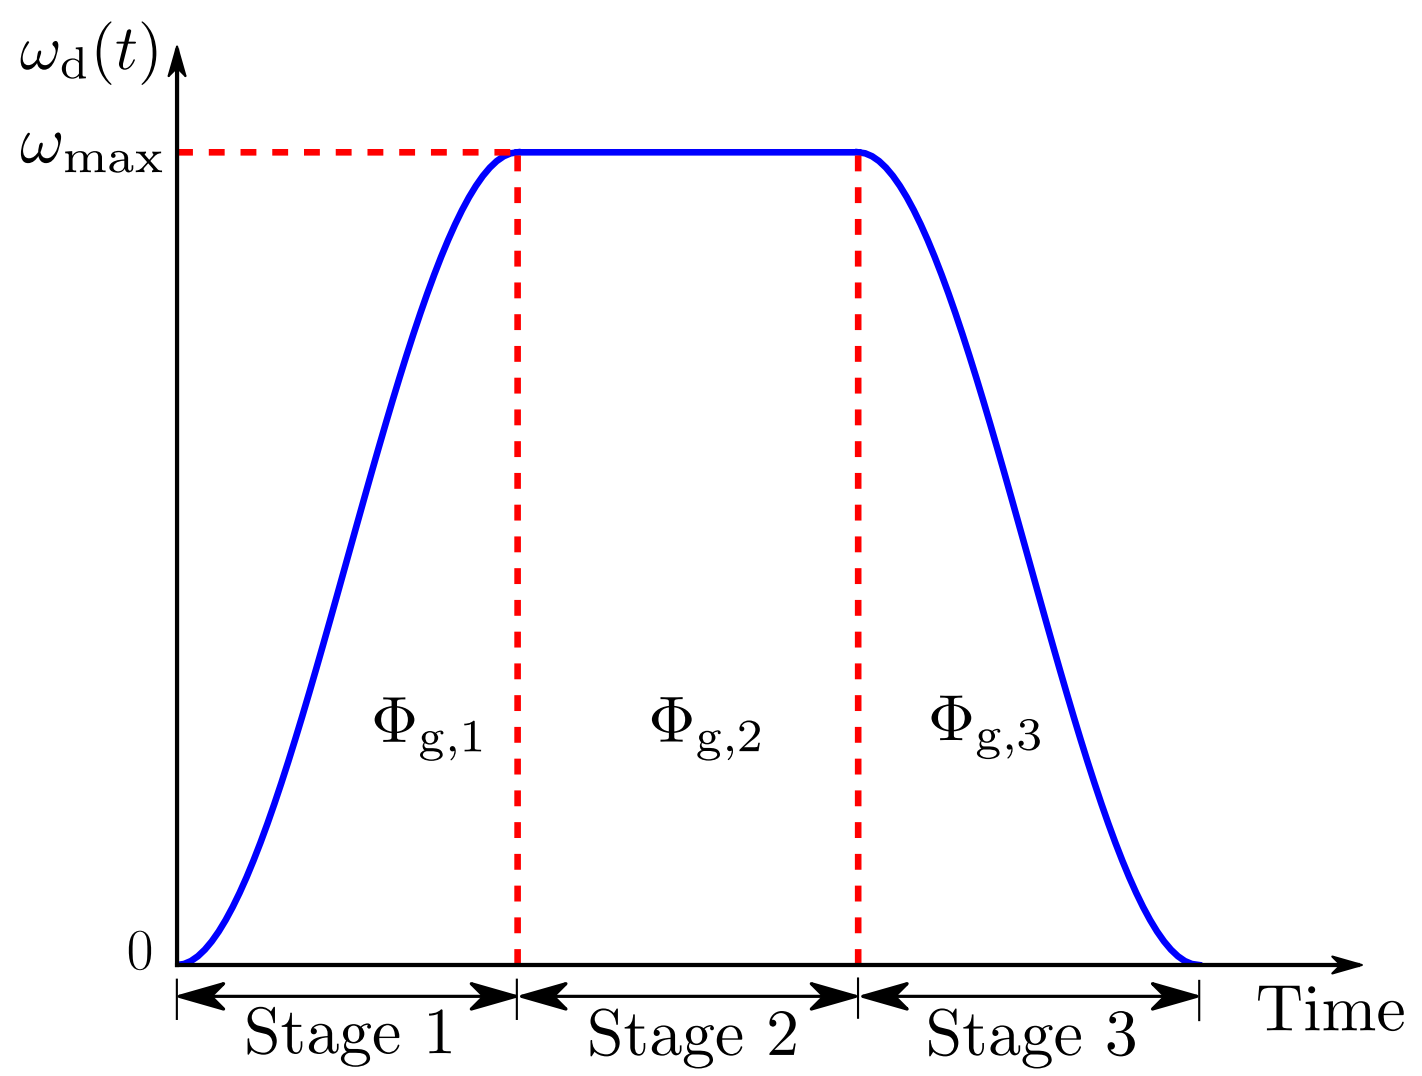
\includegraphics[width=\textwidth]{Images/Flip/Closed_Loop_a}
         \caption{The reference of the angular velocity.}
         \label{closed_loop_a}
     \end{subfigure}
     \hfill
     \begin{subfigure}[b]{0.45\textwidth}
         \centering
         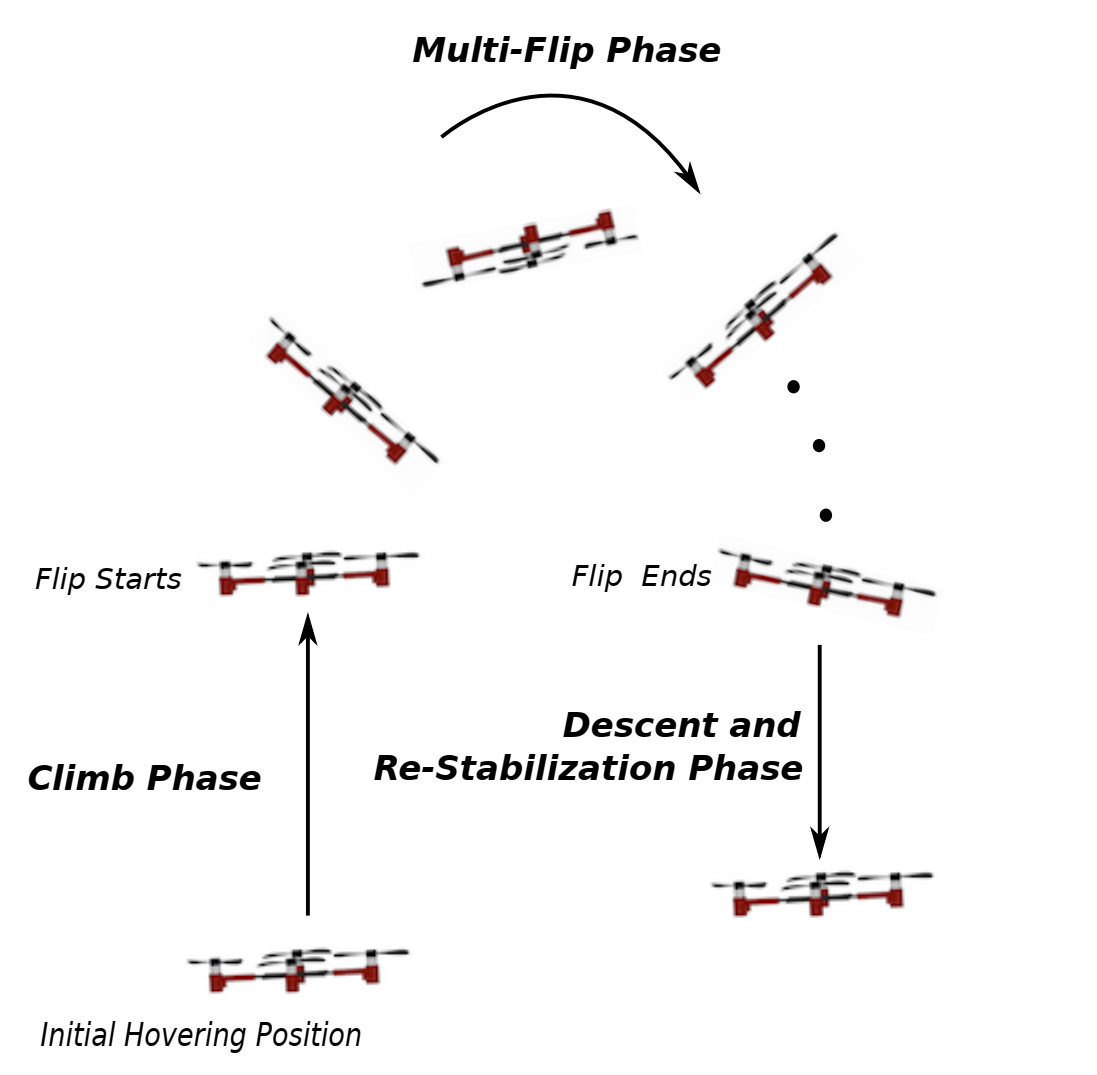
\includegraphics[width=0.8\textwidth]{Images/Flip/Closed_Loop_b}
         \caption{The stages of the multi-flip maneuver.}
         \label{closed_loop_b}
     \end{subfigure}
        \caption{The reference of the flipping speed and the different flipping phases. \cite{Chen2016}}
        \label{closed_loop_c}
\end{figure}

	\item Three distinct control methods to track the reference of the angular speed, which are then compared in terms of the root mean square error. First, a linear time-invariant (LTI) has been proposed \cite{Chen2016} as follows. Provided the error of the angular velocity 
	$\textbf{\textsc{e}}_{\omega} = \bm{\omega} - \omega_d \textbf{\textsc{a}}$ and the error of the angular acceleration $\textbf{\textsc{e}}_{\alpha} = F(s) \bm{\omega} - \dot{\omega}_d \textbf{\textsc{a}}$, with F(s) a filter expressed as $F(s) = \lambda s(s+\lambda)^{-1}$, $\lambda >0$, the consequence control law is: 
	
\begin{equation}
	\bm{\tau} = -\bm{K}_{\omega} \textbf{\textsc{e}}_{\omega} - \bm{K}_{\alpha} \textbf{\textsc{e}}_{\alpha}
\end{equation}

In the subsequent works, a backstepping control approach \cite{Chen2017} has been examined to solve the latency issue which is the result of the slow response of the actuators, in addition to an adaptive control law to estimate unknown parameters on the fly \cite{Chen2018}. In the two cases, these methods achieved better performance when compared to the LTI controller. However, they were not able to successfully reduce the oscillation of the angular velocity within the descent and re-stabilization phase.

\end{enumerate}

\noindent Regardless, this series of papers are by far the most successfull and comprehensive work available in literature on performing multi-flip maneuvers with quadrotors.


 \section{Shortcomings of Current Strategies}
 The control approaches for multi-flip maneuvers that have been presented in section {\ref{control_approaches_for_multi_flip_maneuvers}} demonstrate that the implementation of flipping maneuvers is currently addressed as a more complicated version of the classical attitude control problem. But, no attention has been given on the consequent Cartesian path of the center of mass of the quadrotor, nor on an accurate depiction of the climb phase. In fact, within the first stage, the maximum thrust is established in order to acquire sufficient height. However, none of the works presented above deals with comprehensive altitude analysis in order to give an approximation of the necessary duration for the climb phase. This is mainly done heuristically in experiments. This problem, combined with the fact that the attention is put only on attitude planning and control, results in a totally erratic trajectory for the quadrotor. Thus, it is important to be able to predict the consequent trajectory of the quadrotor during a flipping maneuver. Because, this will help to keep the quadrotor safe, particularly in complex outdoor settings.
 
 
\newpage

 \chapter{Trajectory optimization} 
  
 
 In order to understand what trajectory optimization means, an example of a moving satellite between two planets can be considered.  The term \textit{trajectory} is used to depict the path that the satellite takes between the two planets. Generally, this path would incorporate both the state (position and velocity) and control (thrust) in function of time. the term \textit{trajectory optimization} alludes to a set of  approaches that can be utilized to identify the best trajectory option, generally by choosing the inputs to the system, also known as \textit{controls}, as functions of time.   
 
 \section{The trajectory optimization problem}

\subsection{Formulation of The Optimization Problem} 
 
 The are numerous ways to formulate a trajectory optimization problem(\cite{Betts1998}, \cite{Patterson2013}  \cite{Rao2009}). The main focus will be on single-phase continuous-time trajectory optimization problems. This means that the dynamics of the system are continuous along the full trajectory. Thus, multi-phase methods are outside the scope of this paper and interested readers are referred to \cite{Rao2009} for a more general framework.
 
 
\noindent Generally, an objective function includes two distinct terms: a boundary objective $J$ and a path integral about the full trajectory, with the integrand $w$ . A problem that is containing both terms is considered to be in \textit{Bolza form}. Moreover, a problem only having the integral term is considered to be in \textit{Lagrange form}, and a problem only having the boundary term is considered to be in \textit{Mayer form}. 
 

 
 
 
 
  \begin{equation}\label{trajectory_optimization_function}
 \min\limits_{t_0,t_F,\bm{x}(t),\bm{u}(t)} \underbrace{J \big(t_0,t_f,\bm{x}(t_0),\bm{x}(t_F)\big)}_\text{Mayer Term} + \underbrace{\int_{t_0}^{t_F} w(\tau, \bm{x}(\tau),\bm{x}(\tau),\bm{u}(\tau)) d \tau}_\text{Lagrange Term}
 \end{equation}
 
\noindent In optimization, the term \textit{decision variable} is used to depict the variables that will be adjusted through the optimizer to minimize the objective function. As an example, the decision variables in equation (\ref{trajectory_optimization_function}) are the initial and final time ($t_0, t_f$) in addition to the trajectories of the state and the control input $(\bm{x}(t),\bm{u}(t))$.
Numerous limits and constraints are imposed on the optimization problem at hand, which are detailed in the following equations (\ref{system_dynamcics_equation_tr}-\ref{bound_on_final_state}). 

The first, and possibly the most crucial of all the imposed constraints is the system dynamics, which are generally nonlinear and depict how the system varies with time.
\begin{equation}\label{system_dynamcics_equation_tr}
	\bm{\dot{x}} = \bm{f}\big(t,\bm{x}(t),\bm{u}(t)\big) \space{\hspace{2cm} \textbf{system dynamics}}
\end{equation}
 

\newpage 
 
\noindent Then, there is the path constraint, which implements limitations along the trajectory. As an example, a path constraint can be utilized to maintain the foot of a humanoid robot above the ground in the course of it performing a step.
 
 
\begin{equation}
	\bm{h}\big(t,\bm{x}(t),\bm{u}(t)\big) \leq 0 \space{\hspace{2cm} \textbf{path constraint}}
\end{equation}
 
 
\noindent Another crucial type of constraint is a nonlinear boundary constraint, which imposes limitations of the initial and final state of the system. As an example, this type of constraint can be utilized to make sure that the step of a humanoid robot is periodic.
 
\begin{equation}
	\bm{g}\big(t_0,t_F,\bm{x}(t_0),\bm{x}(t_F)\big) \leq 0 \space{\hspace{2cm} \textbf{boundary constraint}}
\end{equation}
 
 Typically, there are constant limits on the state and the control. For instant, a 6-degrees of freedom (6-DOF) serial anthropomorphic robot  could have limitations on the angles, angular rates, and torques that could be applied throughout the entire trajectory. 
 
 \begin{align}
 \bm{x}_{low} &\leq \bm{x}(t) \leq \bm{x}_{upp} \space{\hspace{2cm} \textbf{path bound on state}} \\
 \bm{u}_{low} &\leq \bm{u}(t) \leq \bm{u}_{upp} \space{\hspace{2cm} \textbf{path bound on control}} 
 \end{align}

Lastly, it is generally crucial to incorporate particular limitations on the initial time $t_0$, the final time $t_F$ and the state $\bm{x}(t)$. These types of constraints can be used to make sure that the solution to a trajectory planning problem attains the goal inside some desirable time window, alternatively it attains some target region in state space.


\begin{align}
t_{low} \leq t_0 < t_F &\leq t_{upp} \text{\hspace{2.35cm} \textbf{bounds on initial and final time}}\\
\bm{x}_{0,low} \leq t_0 < \bm{x}(t_0) &\leq \bm{x}_{0,upp} \text{\hspace{2cm} \textbf{bound on initial state}}\\
\bm{x}_{F,low} \leq t_0 < \bm{x}(t_F) &\leq \bm{x}_{F,upp} \text{\hspace{2cm} \textbf{bound on final state}}\label{bound_on_final_state}
\end{align}
 
 
 \subsection{Direct Collocation Method}
 
 The majority of the methods for solving trajectory optimization problem can be categorized as \textit{direct} or \textit{indirect} methods. In this paper, the main focus will be on direct methods,  however a brief overview will on indirect collocation methods will be provided. The main idea of a direct method is that it discretizes the trajectory optimization problem and converts it into a nonlinear program. This conversion procedure is named \textit{transcription}. This is why the direct collocation methods are also known as \textit{direct direct transcription methods.} Generally, direct transcription methods are capable of discretizing a continuous trajectory optimization problem by estimating all the continuous functions of the problem as polynomial splines. A \textit{spline} is a function which consists of a series of polynomial segments. Polynomials are utilized since they have two crucial characteristics:
 
 \begin{enumerate}
 	\item They can be described by using a small and finite  group of coefficients.
 	\item It is simple to calculate integrals and derivatives of polynomials in function of these coefficients.
 \end{enumerate}
 Throughout this paper, two direct collocation methods will be discussed in detail: \textit{trapezoidal} collocation and \textit{Hermite-Simpson} collocation. Moreover, other direct collocation methods will be briefly covered, such as the direct single shooting method, the direct multiple shooting method and the orthogonal collocation method.
 
 \newpage
 
 \subsection{Nonlinear Programming}
 
 The majority of the direct collocation methods transcribe a continuous-time trajectory optimization problem to a nonlinear problem. A non-linear program is a specific term provided to a constrained parameter optimization problem that contains nonlinear elements in either the objective function or the constraint function. A general expression for a nonlinear program is provided below:
 
  \begin{mini}|s|
{\bm{z}}{ J(\bm{z})}
{}{}
\addConstraint{\bm{f}(\bm{z})=\bm{0}}
\addConstraint{\bm{g}(\bm{z})\leq\bm{0}}
\addConstraint{ \bm{z}_{low}\leq \bm{z} \leq \bm{z}_{upp}}
{}
\label{optim_problem}
\end{mini}

Sometimes, a direct collocation method can result in a linear or quadratic program instead of a non-linear program. This occurs if the constraints (including the dynamics of the system) are linear and the objective function is linear (which results in a linear program) or quadratic (which results in a quadratic program). Linear and quadratic programs are both far easier to tackle than nonlinear programs, rendering them attractive for real-time applications, specifically in robotics.
 
 \section{Trapezoidal Collocation Method}
 
 Trapezoidal collocation operates by transcribing a continuous-trajectory optimization into a non-linear program. This is performed by utilizing trapezoidal quadrature, which is also named the \textit{trapezoidal rule} for integration, to transcribe every continuous element of the problem into a discrete approximation. In this section, the trapezoidal method will be thoroughly examined by demonstrating how the transformation is achieved for each element of a trajectory optimization problem.
 
\subsection{Integrals}

Frequently, there are integral expressions in trajectory optimization problems. Generally, they are located in the objective function, however, it is also possible that they could be located in the constraints too. The aim is to approximate the continuous integral $\int w(\cdot) dt$ as a sum $\sum c_k w_k$. The main idea is that the summation just necessitates the value of the integrand  $w(t_k)=w_k$ at the collocation points $t_k$ about the trajectory. This approximation is performed by applying the trapezoid rule for integration between each pair of consecutive collocation points, which produces the equation below, with $h_k=t_{k+1} - t_k$. \cite{Betts2010}
 
 \begin{equation}
 \int_{t_0}^{t_F} w \big( \tau,\bm{x}(\tau),\bm{u}(\tau)\big)d \tau \approx \sum\limits_{k=0}^{N-1} \frac{1}{2} h_k \cdot (w_k + w_{k+1})
 \end{equation}
 
 \newpage
 
\subsection{System Dynamics}

One of the main features of direct collocation method is that it depicts the system dynamics as a set of constraints, referred to as \textit{collocation constraints}. For trapezoidal collocation, the collocation constraints are built by expressing the dynamics of the system in integral form and then approximation of that integral is performed by using trapezoidal quadrature \cite{Betts2010}. 

\begin{equation*}
\dot{\bm{x}}= \bm{f}
\end{equation*}
 
 \begin{equation*}
\int_{t_k}^{t_{k+1}} \dot{\bm{x}}dt = \int_{t_k}^{t_{k+1}} \bm{f}dt
\end{equation*}
 
  \begin{equation*}
\bm{x}_{k+1}-\bm{x}_k \approx \frac{1}{2} h_k \cdot (\bm{f}_{k+1} + \bm{f}_k )
\end{equation*}
 
 This approximation is then implemented between each pair of collocation points: 
 
 \begin{equation}\label{system_dynamics_equation}
 \bm{x}_{k+1} - \bm{x}_k = \frac{1}{2} h_k \cdot (\bm{f}_{k+1} + \bm{f}_k ) \text{\hspace{2cm}}  k \in \ldots(N-1)
 \end{equation}
 
 \noindent It should be noted that $\bm{x}_k$ is a decision variable in the nonlinear program, whereas \\ $\bm{f}_k = \bm{f}(t_k, \bm{x}_k, \bm{u}_k)$ is the outcome of evaluating the dynamics of the system at every collocation point.
 

\subsection{Constraints} 
 
Besides the collocation constraints, which implement the dynamics of the system, there could also be limits on the state and the control, path constraints and boundary constraints. All of these constraints are managed by implementing them at particular collocation points. For instance, simple constraints on state and control can be approximated as follows:

\begin{align}
\bm{x}< \bm{0} \text{\hspace{1cm}} \rightarrow \text{\hspace{1cm}} \bm{x}_k <\bm{0} \text{\hspace{1cm}} \forall k \\
\bm{u}< \bm{0} \text{\hspace{1cm}} \rightarrow \text{\hspace{1cm}} \bm{u}_k <\bm{0} \text{\hspace{1cm}} \forall k 
\end{align}
 
 Path constraints are managed in the same way: 
 
 \begin{equation}
 \bm{g}(t, \bm{x},\bm{u}) < \bm{0} \text{\hspace{1cm}} \rightarrow \text{\hspace{1cm}} \bm{g}(t_k, \bm{x}_k, \bm{u}_k) <\bm{0} \text{\hspace{1cm}} \forall k \\
 \end{equation}
 
 Moreover, boundary constraint are also enforced at the first and last collocation points:
 
 \begin{equation}
 \bm{h}(t_0, \bm{x}(t_0),\bm{u}(t_0)) < \bm{0} \text{\hspace{1cm}} \rightarrow \text{\hspace{1cm}} \bm{h}(t_0, \bm{x}_0, \bm{u}_0) <\bm{0} \text{\hspace{1cm}} \forall k \\
 \end{equation} 
 
 
 When dealing with constraints, the following points must be taked into consideration: 
 
 \begin{itemize}
 	\item Trajectory optimization problems with path constraints are likely to be considerably harder to solve than trajectory optimization problems without path constraints. The details are beyond the scope of this paper. However, they are properly explained by Betts \cite{Betts2010}.
 	\item The limits of the trajectories are always considered as collocation points in trapezoidal collocation. There exist different methods for which the trajectory limits are not considered as collocation points. For these methods, special attention must be given when boundary constraints are being handled (\cite{Benson2006, Garg2010}.
 \end{itemize}
 
 \newpage
 
 
 \subsection{Interpolation}
 
 Trapezoidal collocation operates by approximating the trajectory of the dynamics of the system and the control trajectory as piece-wise linear functions, which are also called \textit{linear splines}, shown in figure \ref{function_approximation_a}. When building a spline, the term \textit{knot point} is utilized to represent every point that combines two polynomial segments. The knot points related to the spline are coincident in the case of trapezoidal collocation.  
 
 
 \begin{figure}[h]
 \centering
 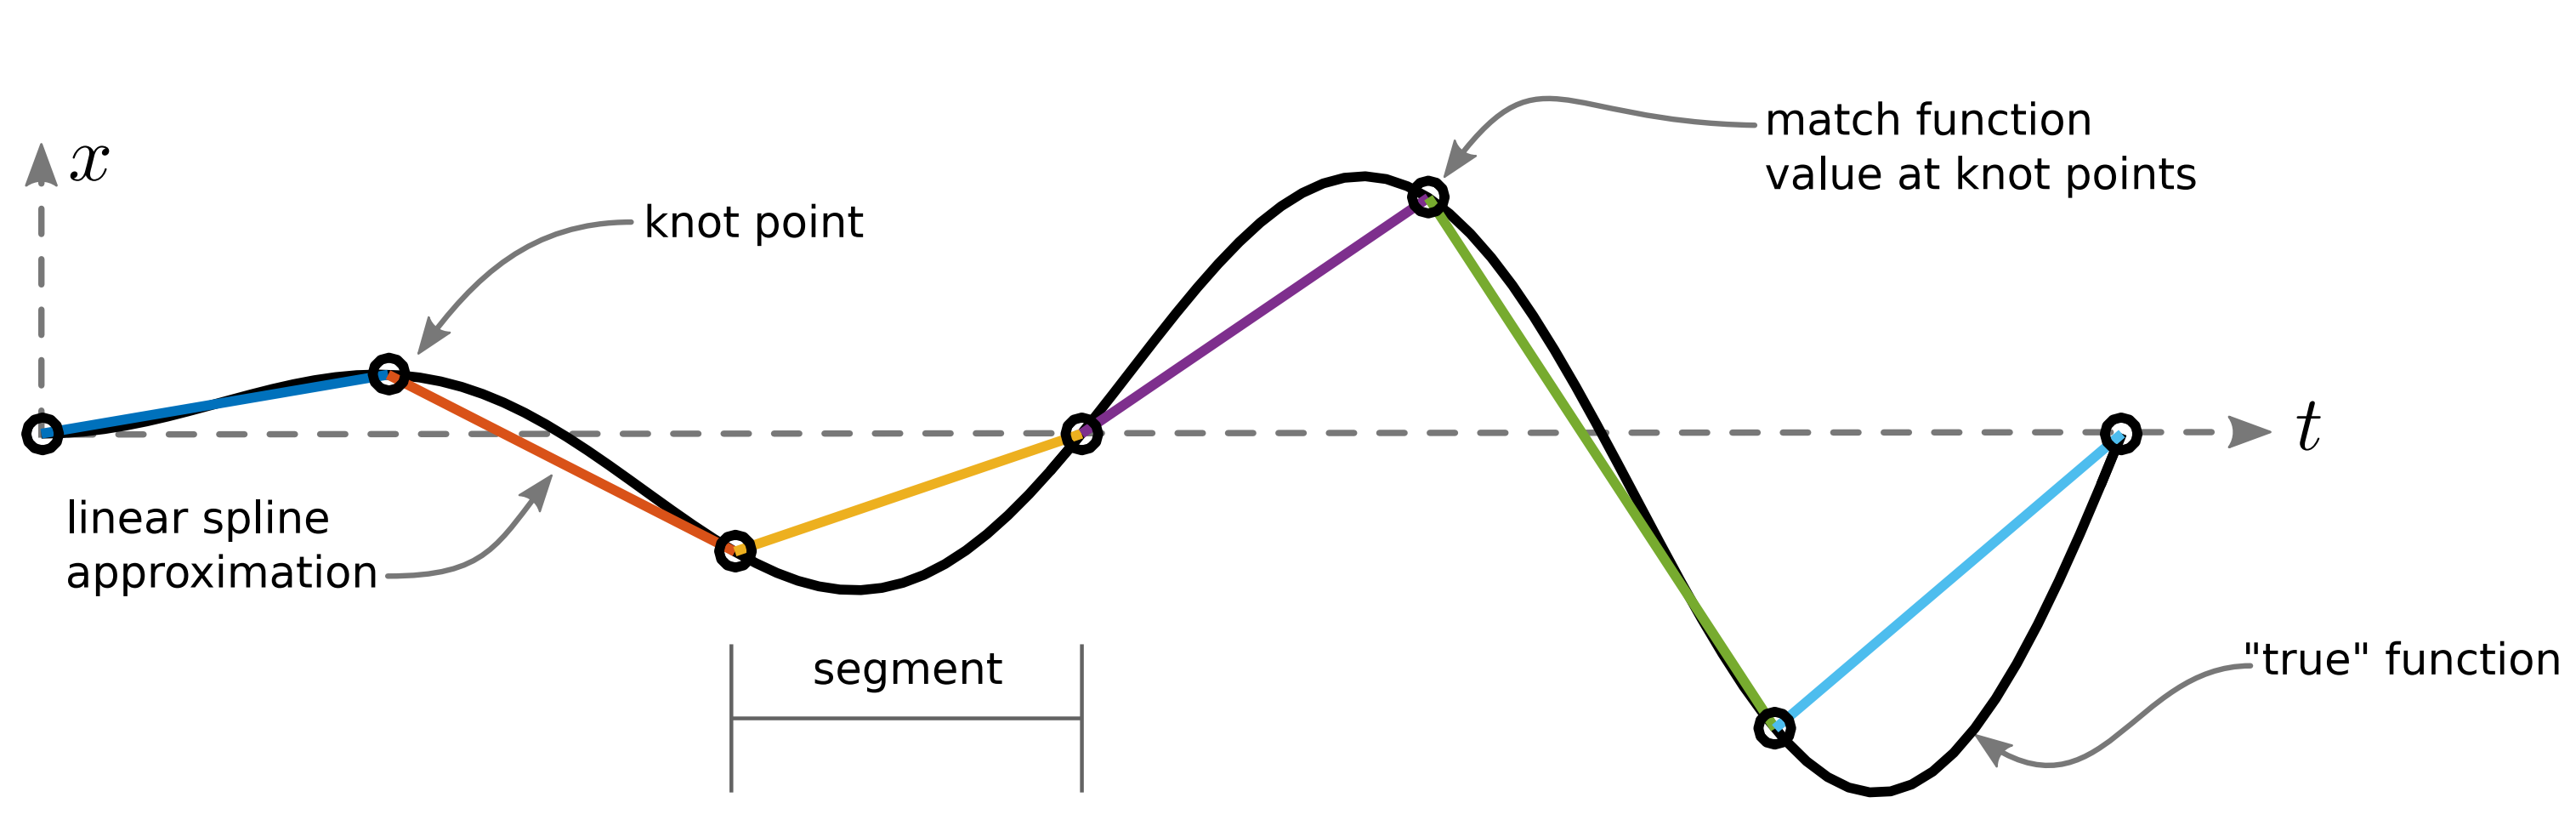
\includegraphics[width=\textwidth]{Images/Trajectory/Function_approximation_a}
 \caption{Function approximation using a linear spline \cite{Kelly2017}.}
 \label{function_approximation_a}
 \end{figure}
 
 
 First, the control strategy must be constructed, which is a simple spline that is linear. Since both the time and control are known at each knot point, then it is easy to derive the expression for $\bm{u}$ on the interval $t \in [t_k,t_{k+1}]$. In order to keep the math readable,$\tau$ and $h_k$ are defined such that:
 
 \begin{equation*}
 	\tau = t-t_k \text{\hspace{2cm}}h_k = t_{k+1} - t_k
 \end{equation*}
   
 Thus, the expression of $\bm{u}$ is the following:
 
 \begin{equation}\label{spline_a}
 	\bm{u}(t) \approx \bm{u}_k + \frac{\tau}{h_k}(\bm{u}_{k+1}-\bm{u}_k)
 \end{equation}
 
 
 The state trajectory is expressed by a \textit{quadratic spline} (a piece-wise quadratic function). This may seem perplexing, however it follows directly from the collocation equations \ref{system_dynamics_equation}. The trapezoidal collocation equations are accurate when the dynamics of the system vary linearly between any two knot points, which is a fact that is used to approximate the dynamics of the system over a single segment $t \in [t_k, t_{k+1}]$ as expressed below.
 
 
 \begin{equation}\label{approximation_of_state_dynamics}
 	\bm{f}(t) = \dot{\bm{x}}(t) \approx \bm{f}_k + \frac{\tau}{h_k}(\bm{f}_{k+1}-\bm{f}_k)
 \end{equation}
 
 However, what is interesting is $\bm{x}$ and not $\dot{\bm{x}}$, thus equation (\ref{approximation_of_state_dynamics}) must be integrated on both sides in order to obtain a quadratic expression for the state.
 
 \begin{equation}
 	\bm{x}(t) = \int \dot{\bm{x}}(t) d \tau \approx \bm{c} + \bm{f}_k \tau + \frac{\tau^2}{2 h_k} (\bm{f}_{k+1}-\bm{f}_k)
 \end{equation}
 
 
Then, the constant of integration $\bm{c}$ can be computed by utilizing the value of the state at the boundary $\tau = 0$  in order to get the final expression of the state.

 \begin{equation}\label{spline_b}
 	\bm{x}(t) \approx \bm{x}_k + \bm{f}_k \tau + \frac{\tau^2}{2 h_k} (\bm{f}_{k+1}-\bm{f}_k)
 \end{equation} 

\newpage 
 
 \begin{figure}[h]
 \centering
 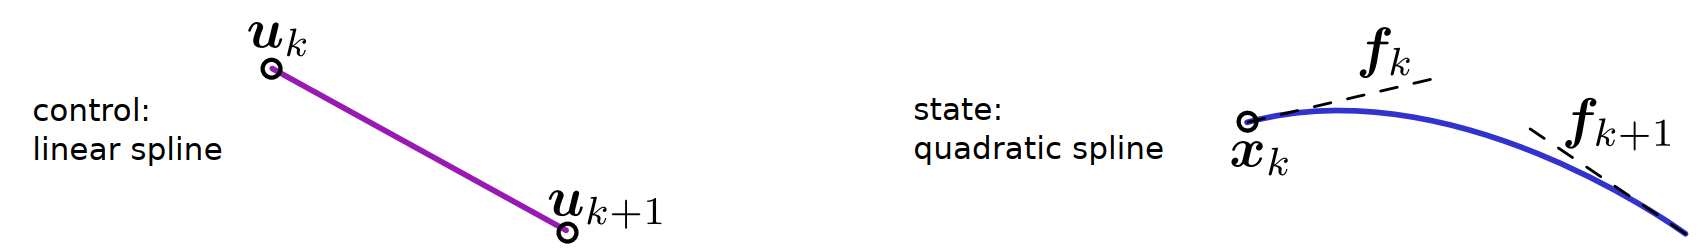
\includegraphics[width=\textwidth]{Images/Trajectory/Trapezoid_Rule}
 \caption{Representation of the linear and quadratic spline segments that are utilizied to approximate the control and state trajectories for trapezoidal collocation.}
 \label{trapezoid_collocation_state_control_fig}
 \end{figure}
 
 
 
\noindent Figure \ref{trapezoid_collocation_state_control_fig} represents how a linear control segment and quadratic state segment are built. The spline equations (\ref{spline_a}) and (\ref{spline_b}) are particularly for trapezoidal collocation, since there is a one-to-one correlation between the collocation equations and the interpolation spline. Generally, if the control is a spline of order $n$, then the state is depicted by a spline of order $n+1$ \cite{Betts2010}.
 
 

\section{Hermite-Simpson Collocation Method}

The Hermite-Simpson collocation is  comparable to the trapezoidal collocation, however it offers a solution that is higher-order accurate. This is due to the fact that trapezoidal collocation approximates the objective function and the dynamics of the system as piece-wise quadratic functions, as shown in figure \ref{function_approximation_b}. An added benefit of the Hermite-Simpson collocation method is that the trajectory is a cubic Hermite spline, which has a first-order derivative which is continuous.


 \begin{figure}[h]
 \centering
 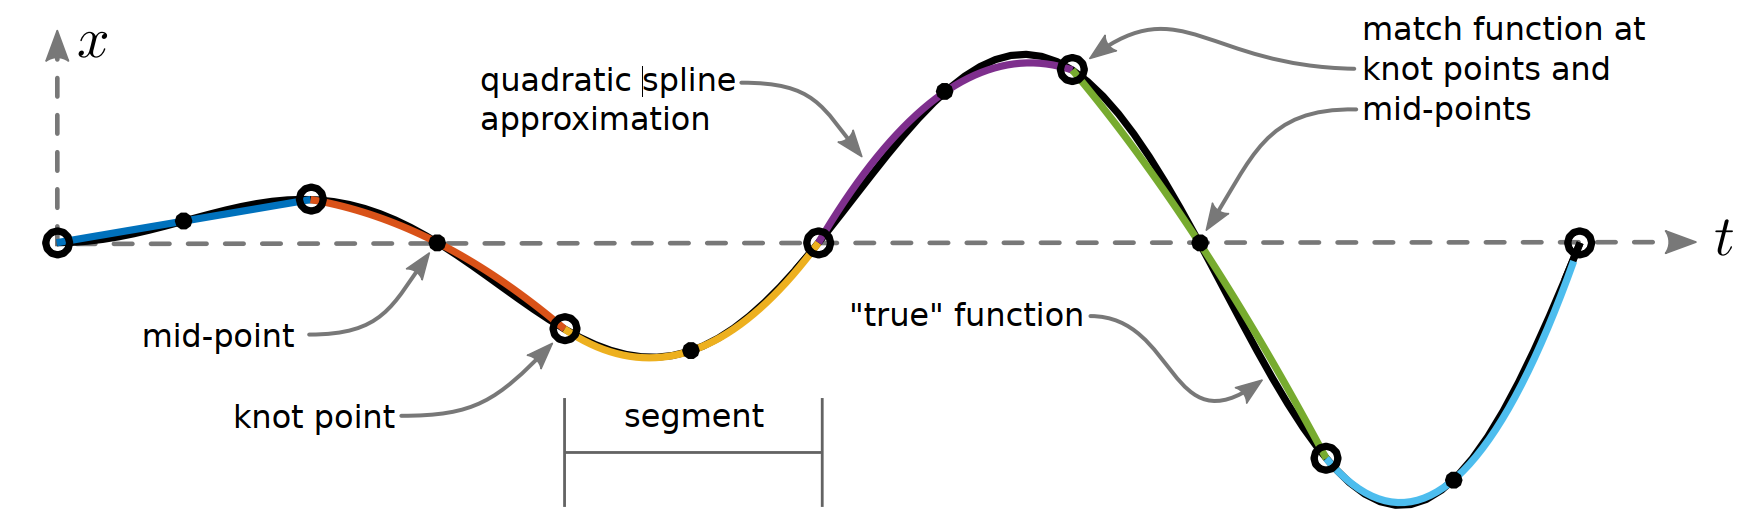
\includegraphics[width=\textwidth]{Images/Trajectory/Function_approximation_b}
 \caption{Function approximation using a quadratic spline.  \cite{Kelly2017}.}
 \label{function_approximation_b}
 \end{figure} 
 
It can be observed that this approximation is significantly more accurate than the linear spline in figure \ref{function_approximation_a}, for the same number of segments.
 
 
 
 \subsection{Integrals}
 
 Integral expressions are regular in trajectory optimization problems, specifically in the objective function. The Hermite-Simpson collocation provide an approximation of the integrals by utilizing the Simpson quadrature. The Simpson quadrature, also called \textit{Simpson's rule} for integration, which operates by approximating the integrand of the integral as a piece-wise quadratic function. This approximation of the integrand is provided below. 
 
\begin{equation*}
\int_{t_0}^{t_f} w(\tau) d \tau \text{\hspace{0.5cm}}  \approx \text{\hspace{0.5cm}}  \sum\limits_{k=0}^{N-1} \frac{h_k}{6} ( w_k + 4 w_{k + \frac{1}{2}} + w_{k+1})
\end{equation*}  
  
  
\subsection{System Dynamics}

Regardless of the collocation method that is being used, the \textit{collocation constraints} are the group of constraints that are built to approximate the dynamics of the system. In the Hermite-Simpson collocation method, these constraints are built by writing the system dynamics in integral form: the change in state between any two knot points $t_k$ must be equal to the integral of the dynamics of the system $\bm{f}(\cdot)$ between those points.
  
  
  \begin{align}
  	\dot{\bm{x}} &= \bm{f} \\
  	\int_{t_k}^{t_{k+1}} \dot{\bm{x}} &= \int_{t_k}^{t_k+1} \bm{f} dt  	\label{continuous_integral}
  \end{align}
  
  The transcription from continuous dynamics to a group of collocation equations takes place when the continuous integral is approximated in  \ref{continuous_integral} with the Simpson quadrature and then implemented between every pair of knot points. 
  
  \begin{equation}\label{first_Hermite_collocation_equation}
  	\bm{x}_{k+1} - \bm{x}_k = \frac{1}{6} h_k(\bm{f}_k + 4 \bm{f}_{k + \frac{1}{2}} + \bm{f}_{k+1})
  \end{equation}
  	
  In fact, for the Hermite-Simpson collocation, a second collocation equation is required in addition to equation (\ref{first_Hermite_collocation_equation}), in order to impose the dynamics of the system. This is due to fact that the dynamics at the mid-point of segment $\bm{f}_{k+\frac{1}{2}}$ are a function of the state $\bm{x}_{k+\frac{1}{2}}$, which is not known \textit{a priori}. Thus, the state of the system can be computed at the mid-point by building an interpolant for the state trajectory  and then assessing it at the mid-point of the interval.
  

	\begin{equation}\label{second_Hermite_collocation_equation}
	\bm{x}_{k+\frac{1}{2}} = \frac{1}{2}( \bm{x}_k + \bm{x}_{k+1}) + \frac{h_k}{8}(\bm{f}_k - \bm{f}_{k+1})
	\end{equation}
  
  This second collocation equation (\ref{second_Hermite_collocation_equation}) is particuar because it can be computed explicitly in function of the state at the knot points. So, it is possible to merge both equations  (\ref{first_Hermite_collocation_equation}) and(\ref{second_Hermite_collocation_equation})  into just one complicated collocation constraint. When the transcription of the dynamics of the system is performed using only this single resulting collocation constraint, then the resulting formulation is said to be in \textit{compressed form}. A different approach is to build an additional decision variable for the state at the mid-point $\bm{x}_{k+\frac{1}{2}}$, and the to use both equation (\ref{first_Hermite_collocation_equation})
  and (\ref{second_Hermite_collocation_equation})
  as constraint equations. When the collocation equations are are formed by utilizing this these two constraint equations, then this pair of equations is considered to be in \textit{separated form}. 
  
  There are numerous trade-offs between the separated and the compressed forms of Hermite-Simpson collocation, which are explained in detail in \cite{Betts2010}. The general rule of thumb is that the separated form is superior when working with a smaller number of segments, while the compressed form is superior when the number of segments is great. Both constraint equations (\ref{first_Hermite_collocation_equation})
and (\ref{second_Hermite_collocation_equation})  can be found in the book of Netts \cite{Betts2010}. 



\subsection{Constraints}


Additionally to collocation constraints, which implement the dynamics of the system, there might also be limits on the state and control, path constraints and boundary constraints. These constraints are all handled by imposing them at particular collocation points. For instance, simple limits on the state of the system and the control are approximated as follows:

\begin{equation}
\bm{x}<\bm{0} \text{\hspace{1cm}}\rightarrow  \text{\hspace{1cm}} \begin{cases}
\bm{x}_k <\bm{0} \\
\bm{x}_{k+\frac{1}{2}}<\bm{0}
\end{cases}
\end{equation}

\begin{equation}
\bm{u}<\bm{0} \text{\hspace{1cm}}\rightarrow  \text{\hspace{1cm}} \begin{cases}
\bm{u}_k <\bm{0} \\
\bm{u}_{k+\frac{1}{2}}<\bm{0}
\end{cases}
\end{equation}

\noindent Path constraints are tackled in a similar manner: they are implemented at all the collocation points as shown below.


\begin{equation}
\bm{g}(t,\bm{x},\bm{u}) < \bm{0} \text{\hspace{1cm}} \rightarrow \text{\hspace{1cm}} \begin{cases}
\bm{g}(t_k, \bm{x}_k,\bm{u}_k) < \bm{0} \\
\bm{g}(t_{k+\frac{1}{2}}, \bm{x}_{k+\frac{1}{2}},\bm{u}_{k+ \frac{1}{2}}) < \bm{0} \\
\end{cases}
\end{equation}

\noindent Boundary constraint are also implemented at the first and last knot points:

\begin{equation}
\bm{h}\big(t_0,\bm{x}(t_0),\bm{u}(t_0)\big) < \bm{0} \text{\hspace{1cm}} \rightarrow \text{\hspace{1cm}} \bm{h}(t_0,\bm{x}_0,\bm{u}_0) <\bm{0}
\end{equation}

\noindent Similarly to the case of trapezoidal collocation, trajectory optimization problems with path constraints always happen to be much more difficult to solve than trajectory optimization problems that do not have path constraints \cite{Betts2010}. In addition, the boundaries of the trajectory are always collocation points. There exist some methods for which the trajectory boundaries are not collocation points. So, special care must be taked when handling boundary constraints for these methods \cite{Benson2006, Garg2010}
  
\subsection{Interpolation}
 
 After solving the nonlinear program, the value of the state of the system and the control trajectories at each collocation point are now known. The subsequent step is to build a continuous trajectory to interpolate the solution between the collocation points. Similarly to what was done in trapezoidal collocation, a polynomial interpolant, which is derived from the collocation equations will be used.
  
 \begin{figure}[h]
 \centering 
 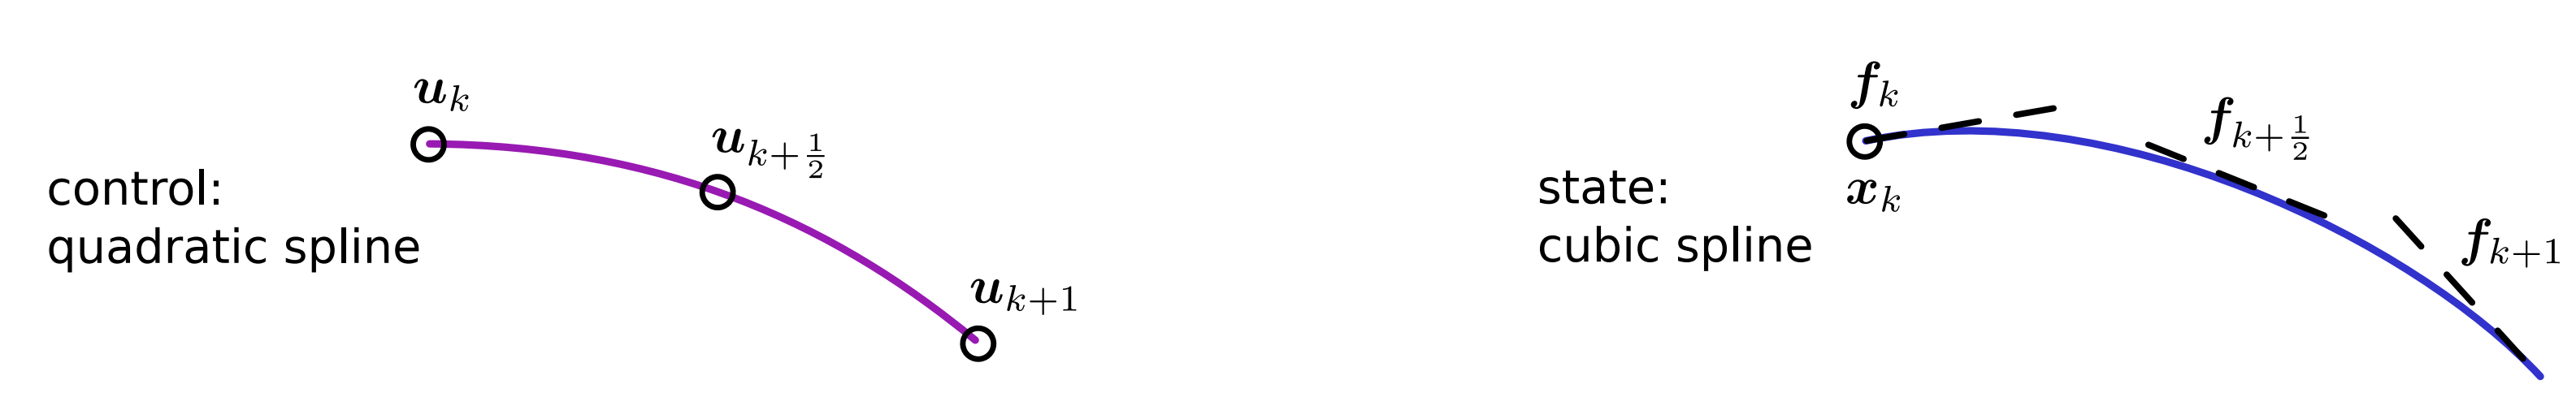
\includegraphics[width=\textwidth]{Images/Trajectory/Hermite-Simpson_Rule}
 \caption{Representation of the quadratic and cubic spline segments that are utilized to approximate the control and state trajectories for Hermite–Simpson collocation.}
 \label{Hermite-Simpson_figure_}
 \end{figure}

Hermite-Simpson collocation operates by using the Simpson quadrature in order to approximate every segment of the trajectory. 
The Simpson quadrature utilizes a quadratic segment, fitted through three equally spaced points in order to approximate the intergrand \cite{Kelly2017}. The general equation for quadratic interpolation is provided in \textit{Numerical Recipes in C} \cite{Press1992}, and it is demonstrated below for a curve $\bm{u}$(t) that passes through 3 points: $(t_A,\bm{u}_A)$, $(t_B,\bm{u}_B)$ and $(t_C,\bm{u}_C)$

\begin{equation}
\bm{u}(t) = \frac{(t-t_B)(t-t_C)}{(t_A-t_B)(t_A-t_C)}\bm{u}_A + 
\frac{(t-t_A)(t-t_C)}{(t_B-t_A)(t_B-t_C)}\bm{u}_B + 
\frac{(t-t_A)(t-t_B)}{(t_C-t_A)(t_C-t_B)}\bm{u}_C
\end{equation}

For this specific case, this equation can be greatly simplified, because the points are uniformly distributed.
Then, the points $k, k+\frac{1}{2}$ and k+1 can be used in place of $A,B$ and $C$ respectively. The next step is to recall from previous sections that $h_k = t_{k+1}-t_k$, and  $t_{k + \frac{1}{2}}=\frac{1}{2}(t_k + t_{k+1})$. And, $\tau$ = $t-t_k$. After doing the proper substitutions and performing some algebra, the following simplified equation for interpolating the control trajectory is the following:

\begin{equation}
	\bm{u}(t) = \frac{2}{h_k^2} (\tau - \frac{h_k}{2})(\tau - h_k)\bm{u}_k - \frac{4}{h_k^2}(\tau)(\tau - h_k)\bm{u}_{k+\frac{1}{2}} + \frac{2}{h_k^2}(\tau)(\tau-\frac{h_k}{2})\bm{u}_{k+1} 
\end{equation}

Hermite-Simpson collocation also describes the dynamics of the system $\bm{f}(\cdot)=\dot{\bm{x}}$ by utilizing quadratic polynomials over each segment. Thus, the quadratic interpolation formula that was developed for the control trajectory can also be implemented to the dynamics of the system.

\begin{equation}\label{state_trajectory_derivative}
	\bm{f}(t) = \dot{\bm{x}} = \frac{2}{h_k^2} (\tau - \frac{h_k}{2})(\tau - h_k)\bm{f}_k - \frac{4}{h_k^2}(\tau)(\tau - h_k)\bm{f}_{k+\frac{1}{2}} + \frac{2}{h_k^2}(\tau)(\tau-\frac{h_k}{2})\bm{f}_{k+1} 
\end{equation}

Generally, the main interest is to obtain an expression for the state trajectory $\bm{x}(t)$ instead of its derivative $\dot{\bm{x}}(t)$. In order to obtain the state trajectory, equation \ref{state_trajectory_derivative} will be integrated, after arranging the expression for it to be in standard polynomial form, the following expression is then obtained.

\begin{equation}
	\bm{x}(t)=\int \dot{\bm{x}}(t)=\int \left[ \bm{f}_k + \bigg(-3 \bm{f}_k + 4 \bm{f}_{k + \frac{1}{2}} -\bm{f}_{k+1}\bigg) \bigg( \frac{\tau}{h_k}\bigg) + \bigg( 2 \bm{f}_k -4 \bm{f}_{k+ \frac{1}{2}} + 2 \bm{f}_{k+1}\bigg)\bigg(\frac{\tau}{h_k}\bigg)^2 \right]dt
\end{equation}


The integral can be calculated by using basic calculus. Then, the constant of integration is solved by using the boundary condition $\bm{x}(t_k) = \bm{x}_k$. The obtained expression is provided below. Moreover, this expression allows the interpolation of the state trajectory.

\begin{equation}
	\bm{x}(t)= \bm{x}_k + \bm{f}_k \bigg(\frac{\tau}{h_k}\bigg) +\frac{1}{2}\bigg(-3 \bm{f}_k + 4 \bm{f}_{k+\frac{1}{2}} - \bm{f}_{k+1}\bigg) \bigg(\frac{\tau}{h_k}\bigg)^2 + \frac{1}{3} \bigg(2 \bm{f}_k -4\bm{f}_{k+ \frac{1}{2}} + 2 \bm{f}_{k+1} \bigg) \bigg(\frac{\tau}{h_k}\bigg)^3
\end{equation}

The interpolant of the state and control trajectories are represented in figure \ref{Hermite-Simpson_figure_}.


\section{Practical Consideration}

In this section, many topics related to trajectory optimization will be covered.


\subsection{Initialization}

Almost every trajectory optimization technique requires a reasonable initial guess in order to start the optimization process. In the best case scenario, a reasonable initialization makes sure that the solver will rapidly converge to the globally optimal solution. In the worst case scenario, it will not allow the non-linear programming solver to solve an otherwise proper optimization problem. The choice of an initial guess can greatly influence which local minimum will the optimizer converge to in the end. In addition, the presence of constraints makes it even worse. In fact, there could be some initial guesses from which the optimization cannot even find a feasible solution. This is an essential problem with non-linear programming solvers since they cannot always find a solution, and if if does find a solution, then it is only ensured to be locally optimal. Furthermore, the best initializations for trajectory optimization problems normally require certain problem-specific information, but there are some general methods that can be helpful. In this manner, initialization is more of an art than a science. A great practice is to test many different initialization methods and check if they all converge the identical local optimum.

One of the most straight forward initialization approaches is to assume that the trajectory is a straight line between the first state and the final state. This method is easy to execute, and will usually work properly for straight forward boundary value trajectory optimization problems.

If an approximate idea of what the problem should look like is known, then this approximate idea can be used as an initial guess for the optimizer. As an example, if a robot is required to perform a back-flip maneuver, then the robot can be sketched out at different points along the back-flip, then the points in the state-space for configuration can be deduced, and then linear interpolation can be used between those points. 

For complex problem, a better approach must be used.  One of the best techniques in that case is to simplify the trajectory optimization problem until a good solution can be reached by using a simple initialization technique. After that, the solution of the simplified problem is then used to initialize the original problem. If this method does not work as intended, then a chain of optimization problems is then built, such that each optimization problem is marginally closer to th desired problem and which utilizes the prior solutions as the initial guess.

\subsection{Mesh refinement}

The direct transcription procedure estimates a trajectory thanks to the use of polynomial spline, which permits the trajectory optimization problem to be transformed into a non-linear program. The collocation constraints in the resulting nonlinear program are functioning as implicit Runge-Kutata integration schemes \cite{Betts2010}. And, similarly to any integration schemes, there exist numerical errors that are linked with the selected time step and method order. Thus , if short time steps (meaning dense meshing) and a high-order method are used, then the output will be an accurate approximation, however this comes at the cost of a high computational load.


Mesh \textit{refinement} is the procedure by which a trajectory optimization problem is solved on a series of distinct collocation meshes, namely \textit{collocation grids}. The mesh grid is related to the choice of discretization along the trajectory. Typically, the initial mesh is unrefined, and contains a small number of collocation points and/or a collocation method of low-order. Succeeding meshes contain more points and/or a collocation method of high-order. This iterating approach is executed in order to have accurate solution with the smallest amount of computational cost. In addition, the solutions that are found by using the initial meshes are simple to solve but inexact, whereas the solutions of the succeeding meshes are more computationally heavy to solve, but they are nonetheless more accurate.



\begin{figure}[h]
\centering
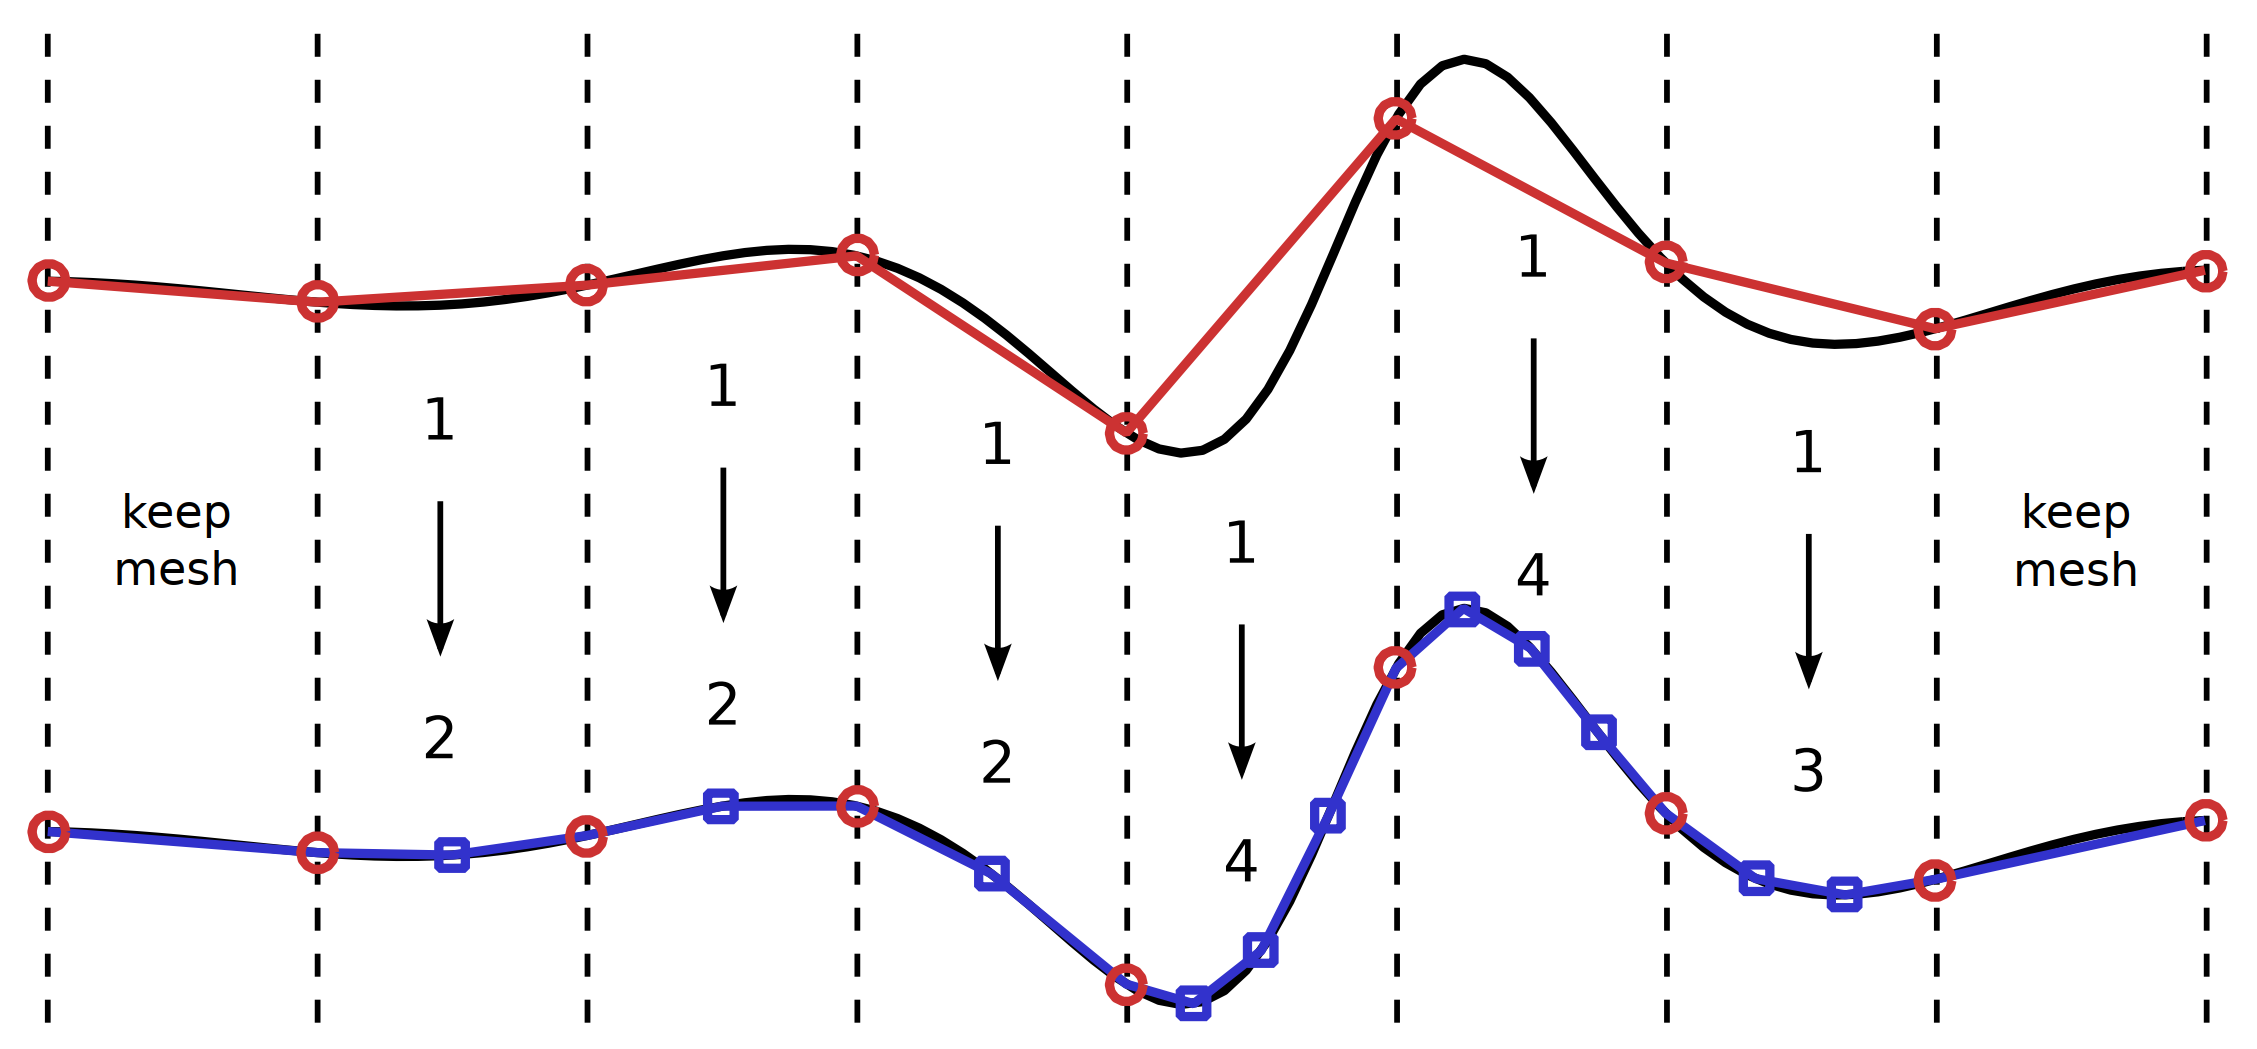
\includegraphics[width=\textwidth]{Images/Trajectory/mesh_refinement}
\caption{Representation of mesh refinement by sub-dividing segments. The number of sub-segments is defined by the maximum error in each segment \cite{Kelly2017}.}
\label{mesh_refinement}
\end{figure}



As can be observed from figure \ref{mesh_refinement}, an easy example is shown in order to represent how the mesh for a linear spline can be improved to provide a representation which is more accurate by simply adding a few points. The segments which contain small errors are not altered, whereas segments with a larger amount of error are sub-divided into 2, 3 or 4 sub-segments for the following iteration.

In more complex mesh-refinement approaches, the accuracy of a certain segment can be enhanced by sub-dividing it or by increasing the order of the polynomial in the segment. These type of algorithms are called \textit{hp-adaptive} meshing. The choice of sub-dividing the mesh or increasing the order of the polynomial is done by examining the error profile inside an individual segment. If there is a steep increase in the error, it means that the the segment must be sub-divided, or the order of polynomial must be increased, for instance, the trapezoidal collocation can be changed to Hermite-Simpson collocation \cite{Kelly2017}.



\subsection{Error Analysis}

There exist two different types of numerical errors that are normally present in the solution of a trajectory optimization problem. These errors are the transcription errors and errors in the solution of the non-linear program. The main focus will be on the accuracy of the transcription procedure, in order to measure how much error has been introduced by the discretization that has been selected. These error estimations can then be used in order to calculate a new discretization. 

There exists various possible ways to measure errors for trajectory optimization problems \cite{Betts2010}. Here, an error estimate will be constructed based on how good the candidate trajectory fulfills the system dynamics between the collocation points. The main idea here is that if the dynamics of the system are exactly satisfied between the collocation points, then the polynomial spline will be considered as an accurate depiction of the system, which means that the non-linear problem is an exact accurate depiction of the original trajectory optimization problem.

A true solution $\bm{x}^*(t),\bm{u}^*(t)$ is not actually known. However, what is known is that it must fulfill accurately the dynamics of the system:

\begin{equation*}
\dot{\bm{x}}^*(t) = \bm{f}(t,\bm{x}^*(t),\bm{u}^*(t))
\end{equation*}

Thus, an expression for the error in the solution to the dynamics of the system throughout the candidate trajectory can then be built. It is crucial that the solution $\bm{x}(t)$ and $\bm{u}(t)$ is computed by using method consistent interpolation \cite{Betts2010}.

\begin{equation*}
	\epsilon (t) = \dot{\bm{x}}(t) - \bm{f}(t,\bm{x}(t), \bm{u}(t))
\end{equation*}

The error $\epsilon(t)$ will be equal to zero at each collocation point and it is non-zero otherwise. Then, the integral of the error can be numerically computed in order to find out how far did the candidate solution have diverted from the actual solution along every dimension of the state. The following expression for the error is generally  computed by utilizing the Rhomberg quadrature \cite{Betts2010}.

\begin{equation*}
	\bm{\eta}_k = \int_{t_k}^{t_{k+1}} | \epsilon (\tau) | d \tau
\end{equation*}

Once the error is found in each state and over each segment of the trajectory, this error can now be utilized in order to find how to re-mesh the trajectory in order for the optimization to converge to an optimal solution that fulfills the continuous dynamics of the system. Interested readers are referred to \cite{Betts2010} and \cite{Darby2011} for more in-depth details on how to compute error estimates and how to accomplish mesh refinement.



\section{Cart-Pole Swing-Up Example}

The cart pole is a system that is made out of a cart that travels along a horizontal track and a pendulum that is not actuated and dangles freely from the cart. A motor is installed on the cart-pole such that it is able to drive the cart ahead or in reverse along the road. It is possible to stimulate the cart in a way such that the pendulum, which is originally hanging below the cart, to swing up and balance above the cart. This part of the paper, the direct collocation method is going to be utilized to compute the minimum-force trajectory that is capable of executing the \textit{swing-up} maneuver.

\subsection{System Dynamics}

The cart-pole is a second-order dynamical system. The position of the cart is provided by $q_1$, and the pole angle is provided by $q_2$. In addition, the control force is provided by $u$. The mass of the cart is given by $m_1$, and the mass of the pole is given by $m_2$. Furthermore, the length of the pole is $l$, and the acceleration due to gravity is $g$, as observed in figure \ref{cart_pole}. Thus, the dynamics of the the cart-pole system are expressed as follows \cite{Kelly2017}:

\begin{equation}\label{ex_eq_1}
	\ddot{q}_1 =\frac{lm_2 \sin(q_2) \dot{q}_2^2 + u + m_2 g \cos (q_2) \sin(q_2)}{m_1 + m_2(1-\cos^2 (q_2))}
\end{equation}


\begin{equation}\label{ex_eq_2}
	\ddot{q}_2 = - \frac{lm_2 \cos(q_2) \sin (q_2) \dot{q}^2_2 + u \cos (q_2) + (m_1 + m_2) g \sin (q_2)}{lm_1 + lm_2(1-\cos^2 (q_2))}
\end{equation}

All conventional trajectory optimization approaches necessitate that the system dynamics be in first-order form. This can be done by including the minimal coordinates $q_1$ and $q_2$ along with their derivatives in the  state space representation of the system, with $\ddot{q}_1$ and $\ddot{q}_2$ which  are defined in  equations (\ref{ex_eq_1}) and (\ref{ex_eq_2}) respectively.

\begin{equation}
\bm{x} = \begin{bmatrix}
q_1\\
q_2\\
\dot{q}_1\\
\dot{q}_2\\
\end{bmatrix}
\text{ \hspace{2 cm} } \dot{\bm{x}} = \bm{f}(\bm{x},u)= \begin{bmatrix}
\dot{q}_1 \\
\dot{q}_2 \\
\ddot{q}_1 \\
\ddot{q}_2 \\
\end{bmatrix}
\end{equation}

\begin{figure}[h]
\centering
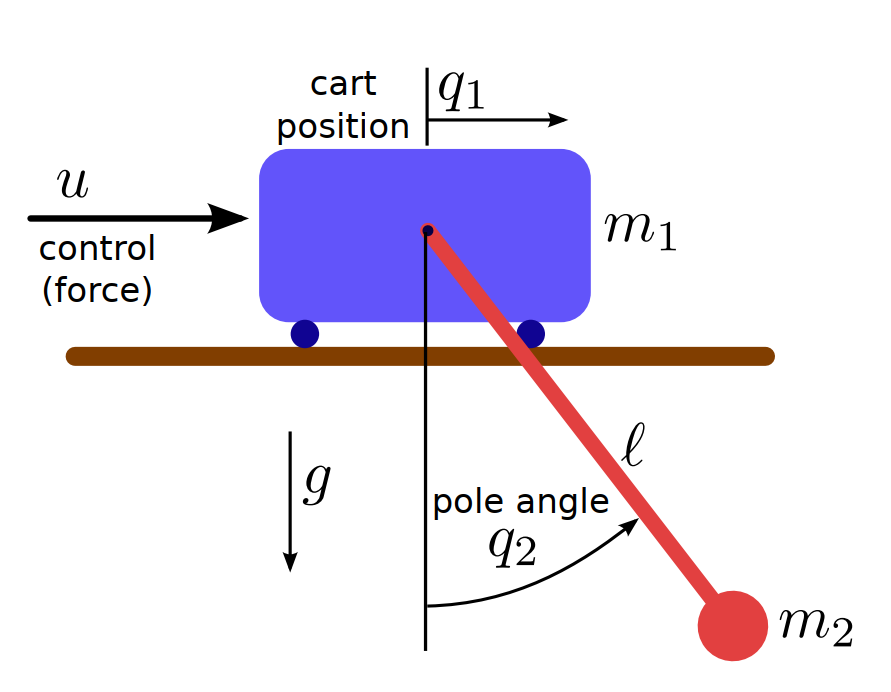
\includegraphics[width=0.5\textwidth]{Images/Trajectory/cart_pole}
\caption{Representation of the cart-pole problem \cite{Kelly2017}.}
\label{cart_pole}
\end{figure}

\newpage

\subsection{Objective function}

One of the most general objective functions that can be used in trajectory optimization problems is the integral of the control input squared.

\begin{equation}\label{objective_function}
J = \int_0^T u^2 (\tau) d \tau
\end{equation}

This objective (\ref{objective_function}) is generally used because it usually results in smooth trajectories. And this characteristic is desirable because most of the majority of the transcription approaches presume that the solution of the optimization problem is properly estimated by a polynomial spline. So, a problem which contains a smooth solution can be solved faster and in a more exact manner than a problem which contains a solution which is not smooth. In addition, smooth trajectories are usually simpler to stabilize with standard controllers when applied on a real system.

\subsection{Boundary Constraints}

Various trajectory optimization problems contain \textit{boundary constraints}, which limit  the system state at the boundaries of the trajectory. In the example, the full state of the cart-pole system will be constrained at the initial and the final points of the trajectory. Presuming that it is desired that the cart must start in the center on the railroad, and it must traverse a distance $d$ while it is performing the swing-up operation. Thus, the boundary constraints in this situation (which are constant) are provided below.

\begin{multicols}{2}
 
\begin{equation*}
\begin{aligned}
q_1(t_0) = 0 \\
q_2(t_0) = 0 \\
\dot{q}_1(t_0) = 0 \\
\dot{q}_2(t_0) = 0 \\
\end{aligned}
\end{equation*}

\columnbreak

\begin{equation*}
\begin{aligned}
q_1(t_F) = d \\
q_2(t_F) = \pi \\
\dot{q}_1(t_F) = 0 \\
\dot{q}_2(t_F) = 0 \\
\end{aligned}
\end{equation*}

\end{multicols}


\subsection{State and Control Bounds}

The swing-up problem of the cart-pole contains some simple constraints. By looking first at the state space of the cart-pole, it is known that the cart will traverse on a track which has a limited length, so it is required to add a simple constraint which limits the horizontal range that can be traveled by the cart. In addition, the force which is due to the motor (control input) will be bounded by a maximum and a minimum value.
Thus, the following constraint equations are obtained.

\begin{equation}
\begin{aligned}
-d_{max} &\leq q_1(t) \leq d_{max}\\
-u_{max} &\leq u(t) \leq u_{max}
\end{aligned}
\end{equation}

\subsection{Trapezoidal collocation}

Now, all the equations that were derived in the previous sections of this example problem can be combined with the trapezoidal collocation approach in order to express the cart-pole swing-up problem as a nonlinear program as follows.


minimize:

\begin{align}
&J = \sum_{k=0}^{N-1} \frac{h_k}{2}(u_k^2 + u^2_{k+1}) \textbf{ \hspace{4cm} objective function} \\
&\text{decision variables:} \nonumber \\
&\bm{x}_0 \ldots\bm{x}_N \text{\hspace{0.5cm}} u_0 \ldots u_N \\
\text{subject to:} \nonumber \\
&\frac{1}{2} h_k( \bm{f}_{k+1} + \bm{f}_k) = \bm{x}_{k+1} - \bm{x}_k \text{\hspace{1cm} } k \in 0 \ldots (N-1) \textbf{\hspace{1cm} collocation constraints }\\
&-d_{max} \leq q_1(t) \leq d_{max} \textbf{\hspace{4cm} path constraints} \\
&-u_{max} \leq u(t) \leq u_{max} \textbf{\hspace{4cm} path constraints} \\
&\bm{x}_0 = \bm{0} \text{\hspace{0.5cm}} \bm{x}_N=[d,\pi,0,0]^{\intercal} \textbf{\hspace{3.5cm} boundary constraints}
\end{align}


It should be noted that $h_k = t_{k+1} - t_k$. Here, a uniform grid will be used. thus, $t_k = k \frac{T}{N}$, where $N$ is the number of segments that were utilized in the process of transcription. However, this problem can be typically solved on an arbitrary grid, which means that $h_k$ could be different.

\subsection{Hermite-Simpson Collocation}

The Hermite-Simpson collocation method can also be utilized in order to build a nonlinear program for the cart-pole to perform the swing-up maneuver. it is very close to the case of trapezoidal collocation, but the only difference is that it utilizes a quadratic spline instead of a linear spline in order to estimate the control and the dynamics equations. So, in this case, the separated form of the Hermite-Simpson approach will be used. This approach requires that collocation points for the state and the control must be included at the middle of each segment $t_{k+\frac{1}{2}}$.\\

minimize:

\begin{align}
&J = \sum_{k=0}^{N-1} \frac{h_k}{6}(u_k^2 + 4 u_{k+\frac{1}{2}}^2 u^2_{k+1}) \textbf{ \hspace{4cm} objective function} \\
&\text{decision variables:} \nonumber \\
&\bm{x}_0, \bm{x}_{0+\frac{1}{2}} \ldots\bm{x}_N \text{\hspace{0.5cm}} u_0,u_{0+\frac{1}{2}} \ldots u_N \\
\text{subject to:} \nonumber \\
&\bm{x}_{k+\frac{1}{2}} = \frac{1}{2}(\bm{x}_k + \bm{x}_{k+1}) + \frac{h_k}{8}(\bm{f_k}-\bm{f}_{k+1}) \text{\hspace{0.5cm}} k\in 0 \ldots (N-1) \textbf{\hspace{0.5cm} interpolation constraints}\\
&\frac{h_k}{6}(\bm{f}_k + 4 \bm{f}_{k+\frac{1}{2}} + \bm{f}_{k+1}) = \bm{x}_{k+1} - \bm{x}_k  \text{\hspace{1cm}} k\in 0 \ldots (N-1) \textbf{\hspace{1cm} collocation constraints}\\
&-d_{max} \leq q_1(t) \leq d_{max} \textbf{\hspace{4cm} path constraints} \\
&-u_{max} \leq u(t) \leq u_{max} \textbf{\hspace{4cm} path constraints} \\
&\bm{x}_0 = \bm{0} \text{\hspace{0.5cm}} \bm{x}_N=[d,\pi,0,0]^{\intercal} \textbf{\hspace{3.5cm} boundary constraints}
\end{align}

\newpage

\subsection{Initialization}

In the cart-pole problem, the initial and final states are provided, and the goal is to calculate an optimal trajectory between the provided initial and final positions. A trivial and straight-forward initial guess is to assume that the system moves in a linear manner between the initial and final state without any control input. This straightforward guess functions greatly for this problem, even though this initial guess does not satisfy the system dynamics.

\begin{equation}\label{initial_guess}
\bm{x}_{guess}(t) =\frac{t}{\tau} \begin{bmatrix}
d \\
\pi \\
0 \\
0 \\
\end{bmatrix} \text{\hspace{2cm}} u_{guess}(t)=0
\end{equation}


As stated earlier, the problem will be solved with a uniform grid, such that $t_k = k \frac{T}{N}$.  So, the initial guess for every single decision variable in the nonlinear program will be calculated using equation (\ref{initial_guess}) at each knot point $t_k$ (and also for the middle point $t_{k+\frac{1}{2}}$ for the Hermite-Simpson collocation method).

\begin{figure}[h]
\centering
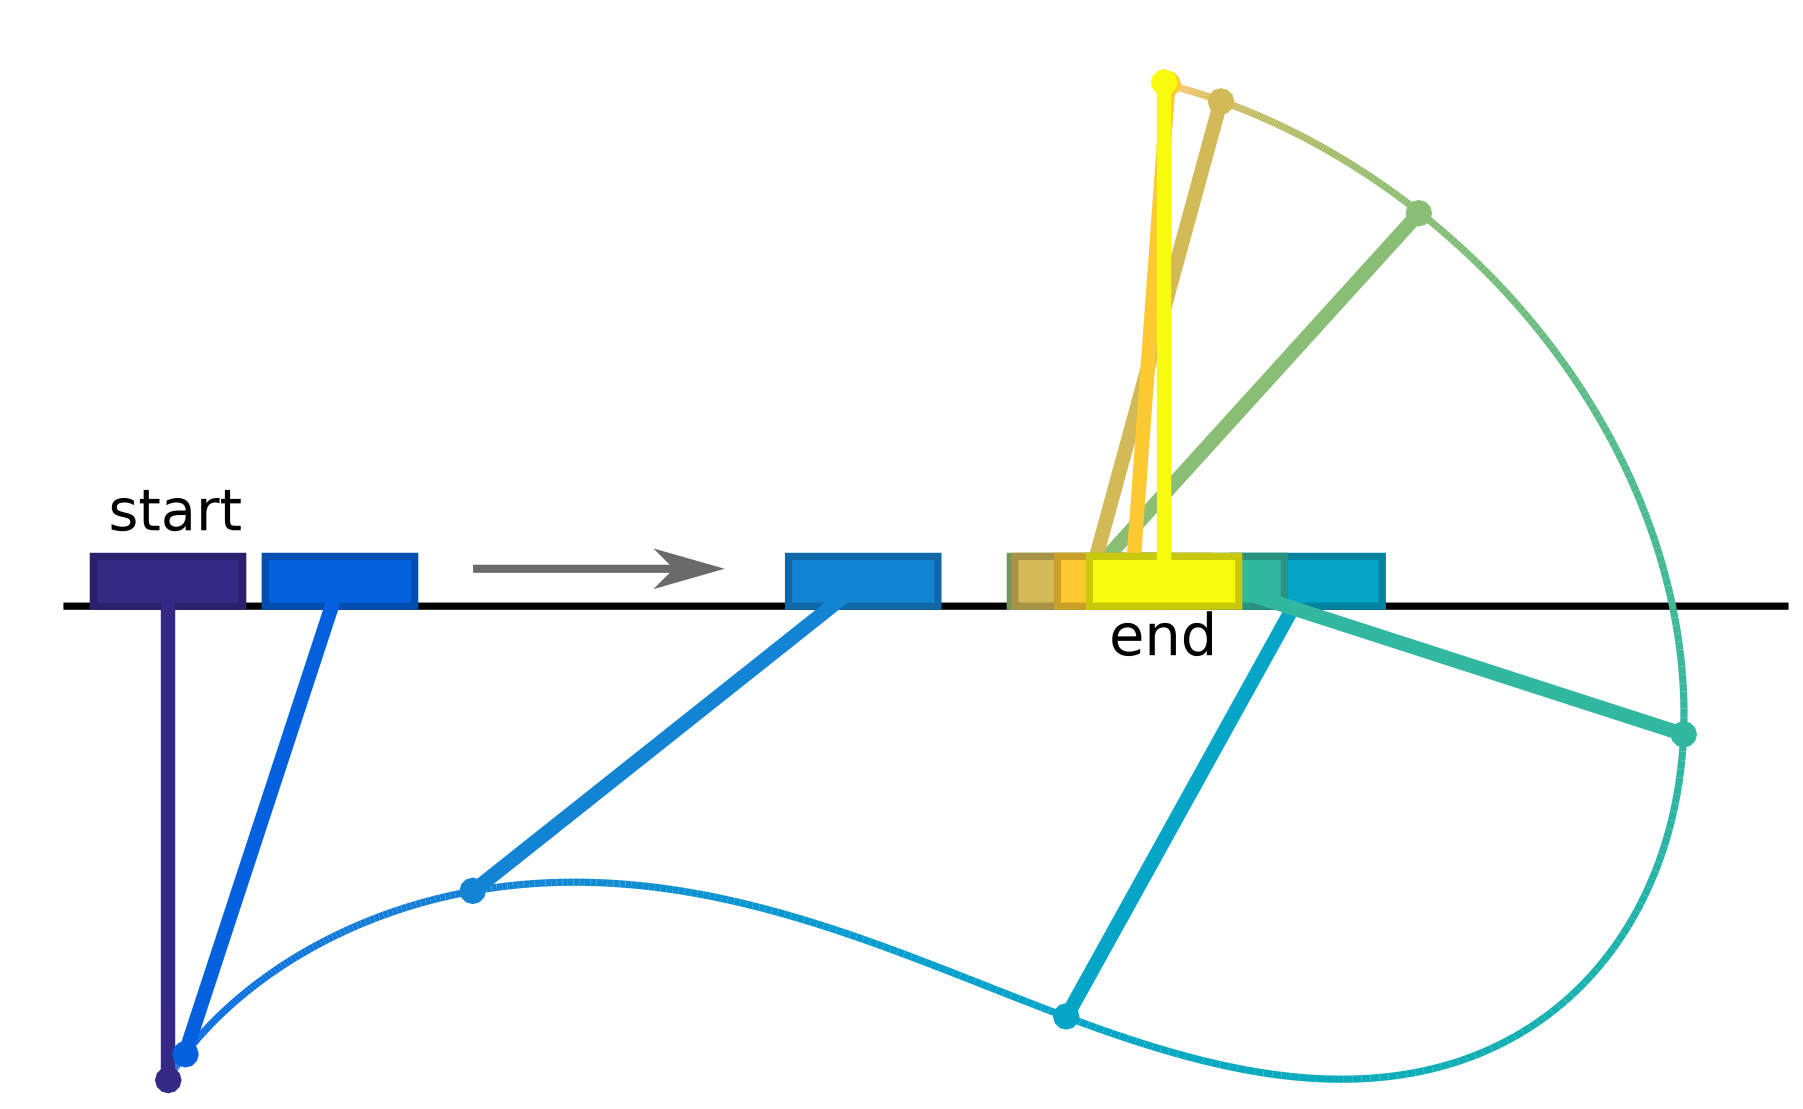
\includegraphics[width=0.6\textwidth]{Images/Trajectory/cart_pole_solved}
\caption{Representation of the optimal trajectory for the cart-pole swing-up example. The frames are uniformly spaced in time, moving from blue (dark) to yellow (light) as the trajectory advances\cite{Kelly2017}. }
\label{trajectory_problem_solution_a}
\end{figure}

\newpage

\subsection{Results}


The optimal swing-up trajectory computed with the Hermite-Simpson collocation by utilizing 25 trajectory segments is presented in this section. The set of parameters that were used to solve the problem are found in \cite{Kelly2017}. The problem was solved by usingthe FMINCON function in MATLAB.

Thus, figure \ref{trajectory_problem_solution_a} represents a stop-action animation of the swing-up movement that is being done, with frames that are uniformly spaced. The identical solution is shown in figure \ref{trajectory_problem_solution_b} which represents plot of the state and the control input in function of time. In the end, figure \ref{trajectory_problem_solution_c} represents the estimated error throughout the trajectory.

It can be observed that the error measurements in the differential equations and the state  increases significantly next to the middle of the trajectory.  At this point, the system is varying quickly as the pole is swinging-up, and the uniform grid is not able to properly approximate the system dynamics. A more complex approach can be used to compute a new grid, given that the segments of the trajectory are smaller next to this point where a quick variation of the system exists.

Parameters were selected in a specific way for this problem such that the system will behave properly. If small alterations are done to the initial guess or the direct transcription approach, then the same solution will still be obtained. However, if some problem parameters were changed, the problem can become much more harder to solve. For instance, if the duration along the trajectory $T$ is increased, then the optimal solution will include several swings of the pole (back and forth) before performing the final swing-up maneuver. Thus, the optimization problem contains many local minima, one for each inexact number of additional swings. The optimization problem can be made more difficult if the limits that are imposed on the actuator $u_{max}$ is reduced. if $u_{max}$ becomes sufficiently small, then the  optimal solution of the problem will no longer be smooth. To solve the problem in that case, the time grid must be re-mesh in order to include supplementary points next to the discontinuities in the trajectory of the input. Another way to solve the discontinuity in the control is to reformulate the problem as a multi-phase problem. However, this is beyond the scope of this master thesis. Interested readers are referred to \cite{Ernesto2013} for a more in-depth explanation. 

\newpage

\begin{figure}[h]
\centering
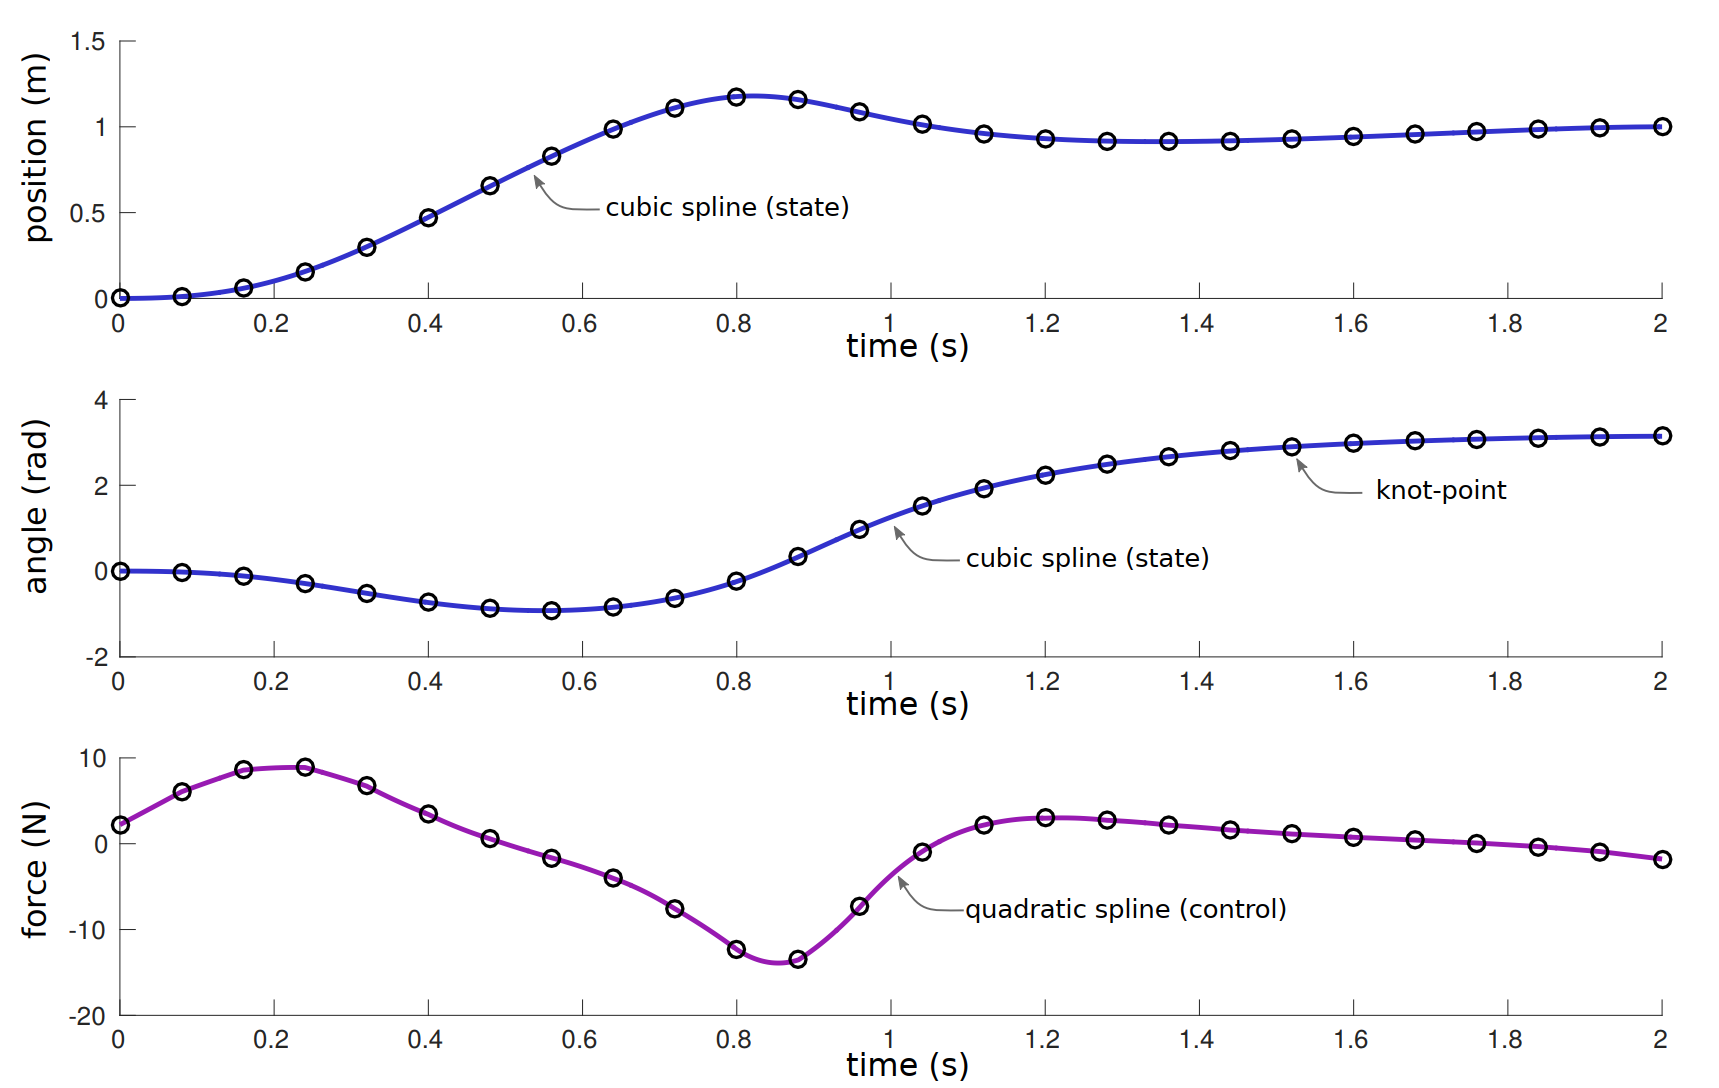
\includegraphics[width=0.75\textwidth]{Images/Trajectory/cart_pole_solved_b}
\caption{Plots showing the optimal trajectory for the cart-pole swing-up example \cite{Kelly2017}. }
\label{trajectory_problem_solution_b}
\end{figure}


\begin{figure}[h]
\centering
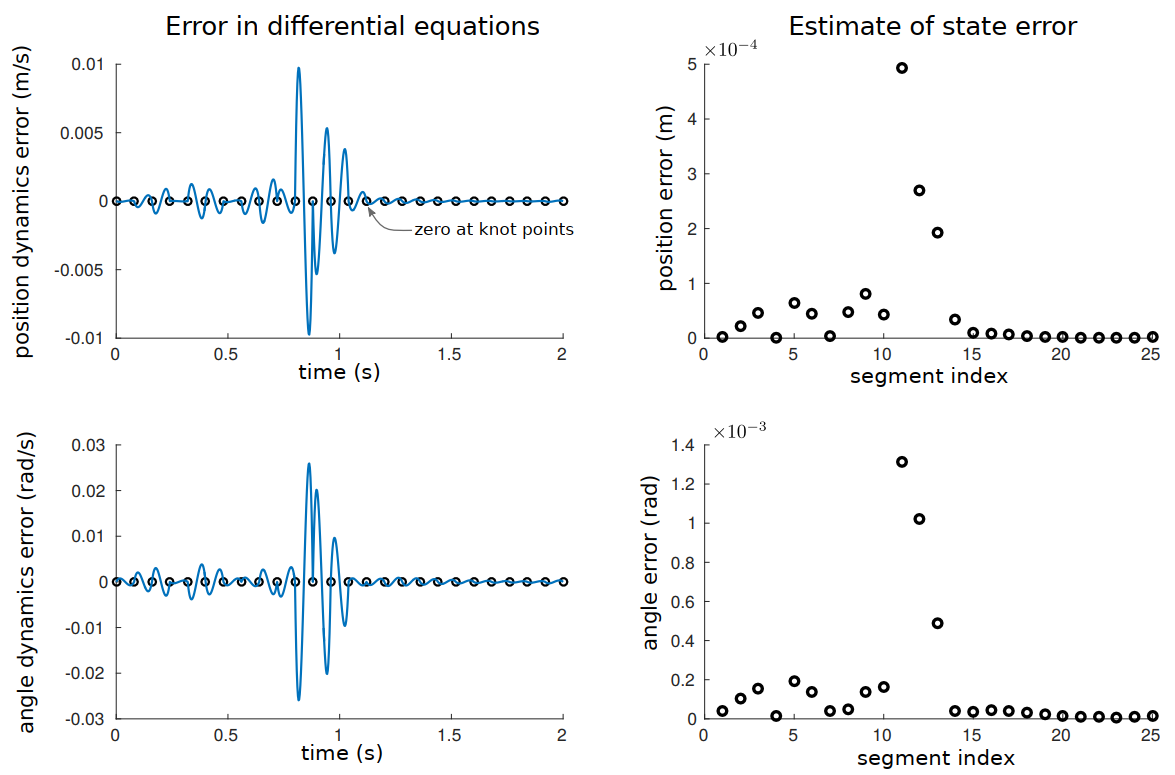
\includegraphics[width=0.75\textwidth]{Images/Trajectory/cart_pole_solved_c}
\caption{Plots showing the optimal trajectory for the cart-pole swing-up example \cite{Kelly2017}. }
\label{trajectory_problem_solution_c}
\end{figure}


\newpage

\section{Existing Trajectory Optimization and Nonlinear Programming solvers}

Some of the available tools that allow to solve the trajectory optimization problem are listed in table \ref{Trajectory_Optimization_software} below:


\begin{table}[h]
\caption{Trajectory Optimization Software}\label{Trajectory_Optimization_software}
\centering
\setlength{\tabcolsep}{10pt} % Default value: 6pt
\renewcommand{\arraystretch}{1} % Default value: 1
\begin{tabular}{||c | c |c |c||}
\hline
Name & License & Interface & Method \\
\hline
\hline
GPOPS-II \cite{Patterson2013} & commerical & MATLAB & direct orthogonal collocation \\
\hline
PSOPT \cite{Becerra2011}& open source & C++ & direct collocation \\
\hline
SOS \cite{Astos2013} & commerical & GUI & direct collocation (methods from \cite{Betts2010}) \\
\hline
DIRCOL \cite{vonStryk1999} & free license & C & direct collocation \\
\hline
DIDO \cite{Elissar2021} & commercial & MATLAB & indirect orthogonal (pseudospectral) collocation\\
\hline
\hline
\end{tabular}
\end{table}

Moreover, a list of non-linear programming solvers are also listed in table \ref{Nonlinear_Programming_Software} below:

\begin{table}[h]
\caption{Nonlinear Programming Solvers}\label{Nonlinear_Programming_Software}
\centering
\setlength{\tabcolsep}{10pt} % Default value: 6pt
\renewcommand{\arraystretch}{1} % Default value: 1
\begin{tabular}{||c |c |c||}
\hline
Name & License & Interface  \\
\hline
\hline
FMINCON \cite{Mathworks2021} & commericial & MATLAB \\
\hline
SNOPT \cite{Gill2006} & commercial & C++ \\
\hline
IPOPT \cite{Wachter2006} & open source & C++  \\
\hline
\hline
\end{tabular}
\end{table}






\newpage 
 
 
 
 
 
 
 
 \chapter*{Conclusion}
 \addcontentsline{toc}{chapter}{Conclusion}
 
 



As can be deduced from the previous chapters, performing multi-flip maneuvers with quadrotors is not an easy task to handle. There are several aspects that must be studied and tuned in order to properly control the quadrotor and perform the multi-flip maneuver. 
First, the dynamic model of the quadrotor must be very thorough and robust in order to have a good representation of the system in simulations and to reduce the errors which result from aerodynamic effects that are usually hard to properly estimate. But, on the other hand, the complexity of the dynamics of the quadrotor must be reduced and simplified in order to satisfy the real-time limitations of the embedded control loop. This is why the very first step to do in this master thesis is to perform the identification of the base dynamic parameters for the quadrotor, since some of the standard parameters of the system have no effect on the dynamic model. So, these irrelevant dynamic parameters can be eliminated and other parameters can also be grouped together, which will greatly reduce the computational cost, regardless of which controller will be used.
Furthermore, several control methods which can be used during this master thesis have been discussed. However, the most interesting control method to be used is model predictive control (MPC), since MPC is a closed-loop controller which will be able to account for modeling errors and disturbances on the system. In addition, MPC will solve an optimization problem at each time step in order to select the optimal control. However, MPC controllers must be properly tuned in order to be able to solve the optimization problem at each time step in real time. This is why simulations are required, since they will be very useful for tuning the control parameters in order to find the best balance between system stability, performance and robustness.
Finally, the trajectory optimization method, which is an open-loop optimization method that was proven to be successful by Marino \cite{Marino2020} for a single-flip maneuver, can be revisited for further experimentation and to add the supplementary constraint of performing the multi-flip maneuvers in  constrained environments.




 
 \paragraph{Planning}
 
The tasks for this master thesis are organized as follows:

\begin{itemize}
	\item Perform the identification of the base dynamic parameters of the quadrotor that will be used for the experiments, namely the \textit{"Crazyflie 2.0"}.
	\item Design a model predictive controller and tune the parameters in a way that the controller can be used on the Crazyflie 2.0 in real-time applications.
	\item Perform simulations using ROS and Gazebo to make sure that the controller is working properly.
	\item Perform real experimentation in the LS2N lab.
	\item Compare the performance of MPC to the performance of trajectory optimization techniques (Closed-loop Vs Open-loop).
\end{itemize}
A Gantt chart of the expected work is provided in figure \ref{Gantt_Chart} below.
\newpage




\begin{figure}[h]
\centering
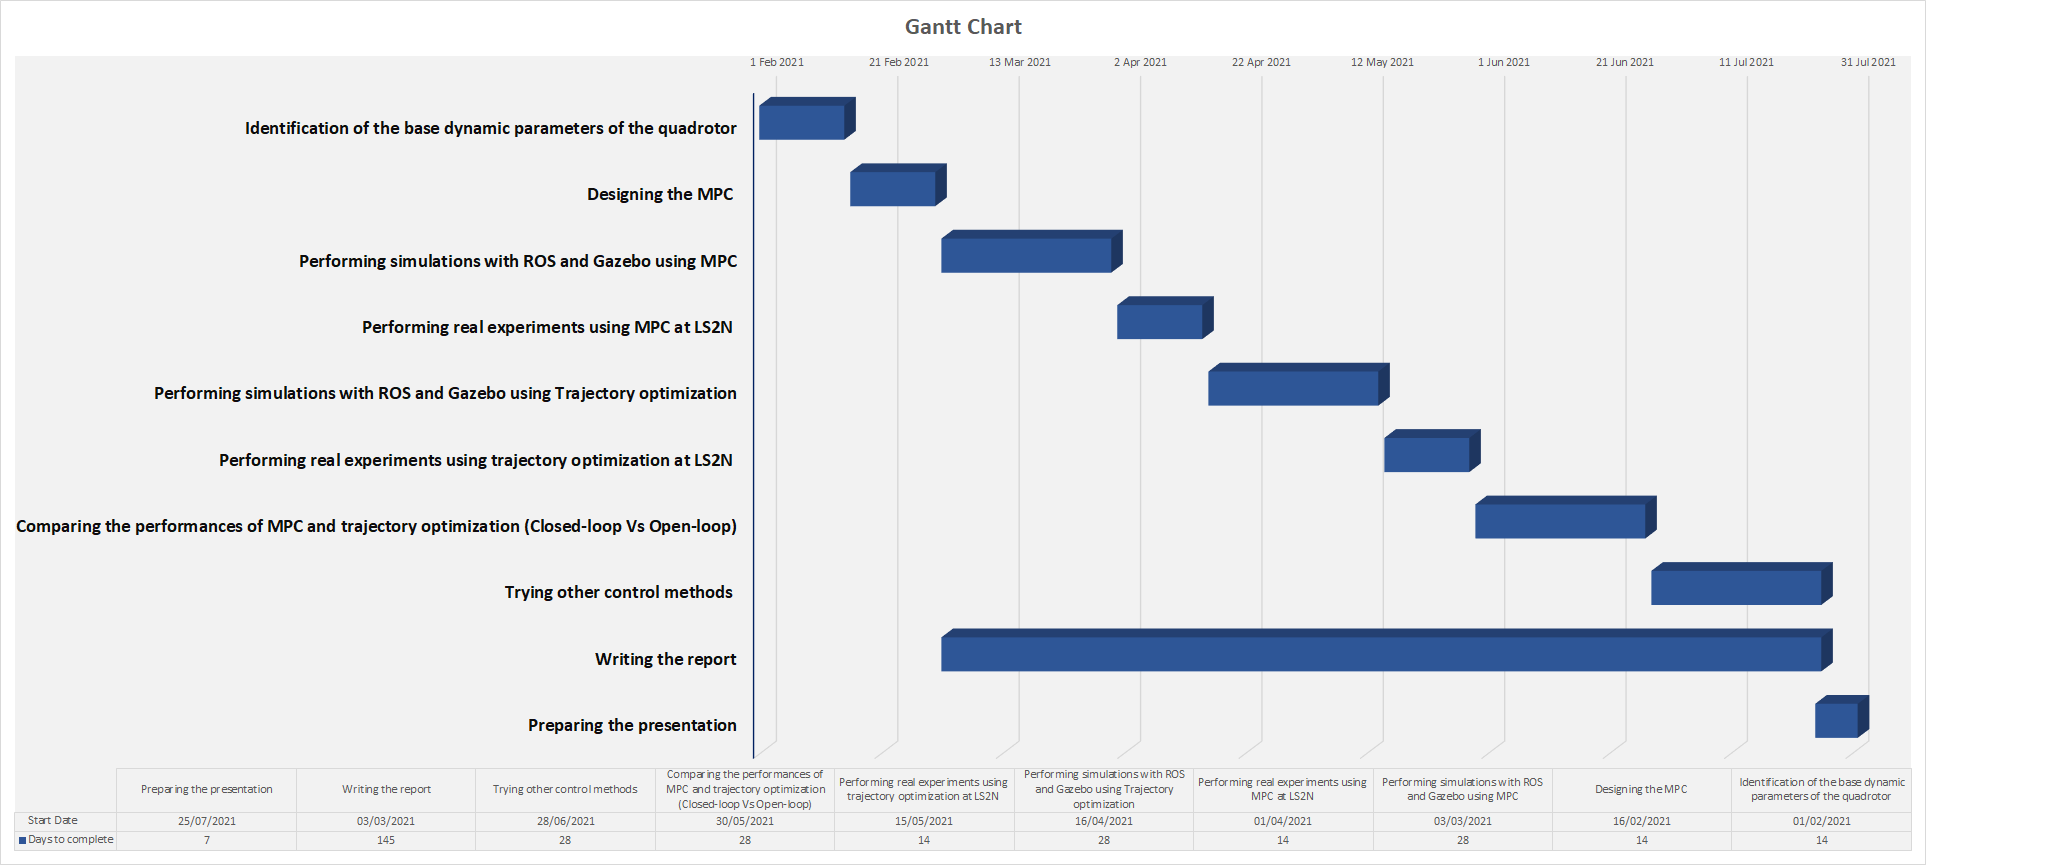
\includegraphics[width=\textwidth]{Images/Planning/Gantt Chart}
\caption{Representation of the expected work to be done during the Master thesis.}
\label{Gantt_Chart}
\end{figure}



 \addcontentsline{toc}{chapter}{Bibliography}
 \nocite{*}
 
 \bibliography{../biblio}


 
\end{document}
